\chapter{Properties of TASE-grown nanowires}
\label{chap:properties}

The critical growth mechanisms and single-facet \hkl{111}\(_B\) growth front stabilisation method were explored and developed in Chapter~\ref{chap:growth}. However, the lack of in-plane \hkl{1 1 1} directions in the \hkl(0 0 1) \acf{soi} wafer on which growth was carried out complicates the analysis of the growth results. The two possible \hkl{1 1 1} facets are tilted and, therefore, yield calculations and contacting of devices become more complex, as the process through which one of the facets is selected for stabilisation is dependent on the shape and orientation of the nucleating crystal on the \acs{si} seed.

This chapter expands on the research my co-authors and I published in \cite{Brugnolotto2023, Brugnolotto2023_2}. 

CHAPTER OVERVIEW

\section{\texorpdfstring{Fabrication on \acs{si}\hkl(1 1 0) \acs{soi}}{Fabrication on Si(110) SOI}}

The fabrication of templates for nanowires and microstructures on the new \hkl(1 1 0) substrate followed the same underlying methodology (see Appendix~\ref{chap:tase}) implemented on the same tools (see Appendix~\ref{chap:tools}) that was used for the samples in Chapter~\ref{chap:growth}. A series of lithography steps, including both \acf{ebl} and uv lithography; deposition steps, including \acf{ald} and \acf{pecvd}; and etching steps, including \acf{rie}, \acf{icp} etching and \acf{tmah} and \acf{hf} etching were employed to define the structures (seed and growth region) enclose them in the template \acs{sio2}, open the template, and finally etch back the sacrificial \acs{si} to expose the seed surface.

\subsection{Template design considerations}


\begin{figure}
    \centering
    \subcaptionbox{
    \hkl(1 1 0) in-plane crystalline directions.
    \label{subfig:110wafer_directions}
    }{
        \tikzsetnextfilename{110wafer_directions}
        \begin{tikzpicture}
            \begin{scope}[scale=0.22]
                \draw (90:11cm) -- (90:13cm);
                \draw[stealth-stealth] (90:12cm) arc [start angle = 90, end angle = -90, radius = 12cm] node[midway, anchor = west]{\qty{180}{\degree}};
                \draw (-90:11cm) -- (-90:13cm);
                \draw (-90:10cm) arc [start angle=270, end angle=358.8, radius=10cm] -- (9.8935cm,-1.065mm) arc [start angle=-135, end angle=-225, radius=1.5mm] -- (9.9987cm,2.13mm) arc [start angle=1.20, end angle=90, radius=10cm];
                \draw[dashed] (90:10cm) arc [start angle=90, end angle=270, radius=10cm];
                \path[decorate,decoration={text along path, text={Repeated by symmetry},text align=center}] (315:11) arc [start angle=315,end angle=45,radius=11];
                \draw[dashed] (90:10cm) -- (0, 0) -- (-90:10cm);
                \draw[-stealth, thick] (0, 0) -- ++ (90:4cm) node[anchor=south east] {\hkl[0 0 1]};
                \draw[-stealth, thick] (0, 0) -- ++ (35.3:4cm) node[anchor=south] {\hkl[-1 1 1]};
                \draw[-stealth, thick] (0, 0) node[anchor=east] {\hkl[1 1 0]} -- ++ (0:4cm) node[anchor=west] {\hkl[-1 1 0]};
                \draw[-stealth, thick] (0, 0) -- ++ (270:4cm) node[anchor=north east] {\hkl[0 0 -1]};
                \draw[-stealth, thick] (0, 0) -- ++ (-35.3:4cm) node[anchor=north] {\hkl[-1 1 -1]};
                \node[mark size=2pt] at (0, 0) {\pgfuseplotmark{diamond*}};
            \end{scope}
        \end{tikzpicture}
    }
    \subcaptionbox{
    \acs{si} seed area before growth.
    \label{subfig:110_etchback}
    }{
        \tikzsetnextfilename{110_etchback}
        \begin{tikzpicture}
            \filldraw[fill=Si_green] (2cm, 0cm) --  node[midway, anchor= north west] {\acs{si}} (2cm, 22mm) -- (4cm, 22mm) -- (4cm, 0cm) node[midway, anchor=west]{{\hkl{1 1 1}}} -- cycle;
            \filldraw[fill=SiO2_blue] (0cm, -10mm) -- (8cm, -10mm) -- (8cm, 0cm) -- (2cm, 0mm)-- (2cm, 22mm) -- (8cm, 22mm) -- (8cm, 32mm) -- (0cm, 32mm) --  node[midway, anchor=west] {\acs{sio2}} cycle; 
            \draw (3.7cm, 22mm) arc [start angle = 180, end angle = 270, radius = 3mm] node[midway, anchor = north east]{\qty{90}{\degree}};
            \draw[-stealth] (6cm, 7mm) node[anchor=north] {\hkl<-1 1 -2>} -- ++ (90:0.8cm) node[anchor=south] {\hkl<1 1 0>};
            \draw[-stealth] (6cm, 7mm) -- ++ (0:0.8cm) node[anchor=west] {\hkl<-1 1 1>};
            \node[mark size=2pt] at (6, 7mm) {\pgfuseplotmark{o}};
        \end{tikzpicture}
    }
    \caption{Crystalline orientations in the \hkl[1 1 0] \acs{soi} wafer. \subref{subfig:110wafer_directions} shows a schematic of the crystalline directions in the plane of the \acs{si} device layer, highlighting its two-fold symmetry. \subref{subfig:110_etchback} highlights the high-symmetry directions in the \hkl{1 1 2} plane containing the chosen \hkl<1 1 1> growth direction and the \hkl[1 1 0] vector defining the wafer orientation. It highlights the vertical \hkl{1 1 1} seed facet.}
    \label{fig:110_wafer_properties}
\end{figure}

An initial evaluation of the crystalline symmetry in the wafer plane is necessary to plan the orientation of the \acf{tase} templates on the wafer surface. Figure~\ref{subfig:110wafer_directions} shows the various in-plane crystalline directions in the top device layer of the \hkl(1 1 0) \acs{soi} wafer employed in the fabrication of all future samples. Unlike its \hkl(001) predecessor, which had a four-fold axis perpendicular to the wafer plane, this \hkl(1 1 0) wafer has a two-fold axis dictating the in-plane symmetry. Therefore, the wafer's notch becomes key to orienting the \acs{tase} structures with the desired crystalline directions.
\par
Figure~\ref{subfig:110_etchback} shows a schematic cross-section of the \acs{tase} structure before growth with colour-coded materials. The \acs{si} seed presents a \hkl{1 1 1} facet forming a \qty{90}{\degree} angle with all the template walls because of the \acs{tmah} etchant used to remove the sacrificial \acl{si}; unlike the \hkl<0 0 1> wafer samples which formed \qty{90}{\degree} angles with the sidewalls (Figure~\ref{subfig:enterprise_etchback}).

\begin{sidewaysfigure}
    \centering
    \subcaptionbox{
    Double comb structure evolution from the comb structure in Figure~\ref{subfig:enterprise_design}.
    \label{subfig:110_design1}
    }{
        \tikzsetnextfilename{110_design1}
        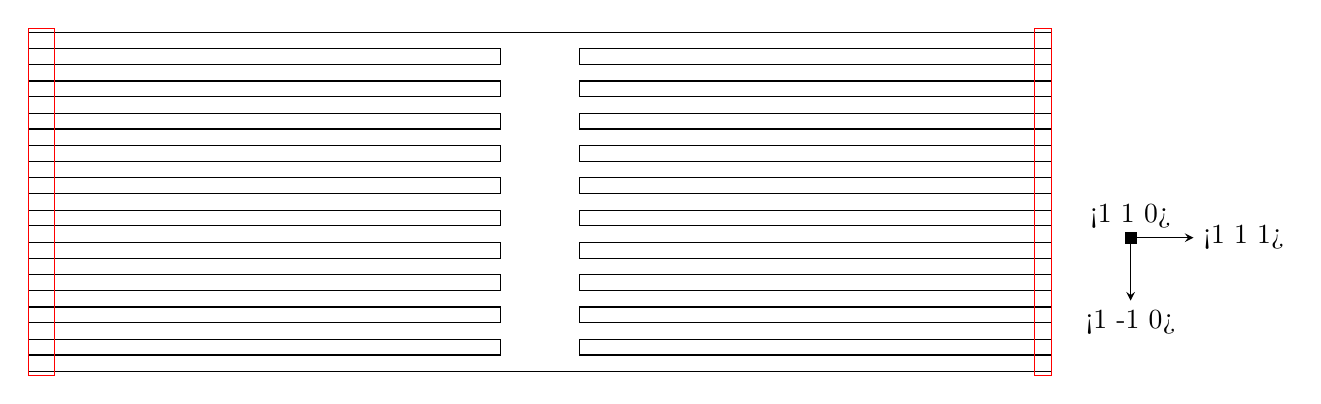
\begin{tikzpicture}
            \begin{scope}[]
                \draw (0, 0) -- ++ (13, 0) -- ++ (0, 0.21) -- ++ (-6, 0) -- ++ (0, 0.2) -- ++ (6, 0) -- ++ (0, 0.21) -- ++ (-6, 0) -- ++ (0, 0.2) -- ++ (6, 0) -- ++ (0, 0.21) -- ++ (-6, 0) -- ++ (0, 0.2) -- ++ (6, 0) -- ++ (0, 0.21) -- ++ (-6, 0) -- ++ (0, 0.2) -- ++ (6, 0) -- ++ (0, 0.21) -- ++ (-6, 0) -- ++ (0, 0.2) -- ++ (6, 0) -- ++ (0, 0.21) -- ++ (-6, 0) -- ++ (0, 0.2) -- ++ (6, 0) -- ++ (0, 0.21) -- ++ (-6, 0) -- ++ (0, 0.2) -- ++ (6, 0) -- ++ (0, 0.21) -- ++ (-6, 0) -- ++ (0, 0.2) -- ++ (6, 0) -- ++ (0, 0.21) -- ++ (-6, 0) -- ++ (0, 0.2) -- ++ (6, 0) -- ++ (0, 0.21) -- ++ (-6, 0) -- ++ (0, 0.2) -- ++ (6, 0) -- ++ (0, 0.21) -- ++ (-13, 0) -- ++ (0, -0.21) -- ++ (6, 0) -- ++ (0, -0.2) -- ++ (-6, 0) -- ++ (0, -0.21) -- ++ (6, 0) -- ++ (0, -0.2) -- ++ (-6, 0) -- ++ (0, -0.21) -- ++ (6, 0) -- ++ (0, -0.2) -- ++ (-6, 0) -- ++ (0, -0.21) -- ++ (6, 0) -- ++ (0, -0.2) -- ++ (-6, 0) -- ++ (0, -0.21) -- ++ (6, 0) -- ++ (0, -0.2) -- ++ (-6, 0) -- ++ (0, -0.21) -- ++ (6, 0) -- ++ (0, -0.2) -- ++ (-6, 0) -- ++ (0, -0.21) -- ++ (6, 0) -- ++ (0, -0.2) -- ++ (-6, 0) -- ++ (0, -0.21) -- ++ (6, 0) -- ++ (0, -0.2) -- ++ (-6, 0) -- ++ (0, -0.21) -- ++ (6, 0) -- ++ (0, -0.2) -- ++ (-6, 0) -- ++ (0, -0.21) -- ++ (6, 0) -- ++ (0, -0.2) -- ++ (-6, 0) -- ++ (0, -0.21);
                \draw[red] (0, -0.05) rectangle (0.333, 4.36);
                \draw[red] (12.777, -0.05) rectangle (13, 4.36);
            \end{scope}
            \begin{scope}[shift={(14cm, 1.7cm)}]
                \draw[-stealth] (0cm, 0cm) -- ++ (-90:0.8cm) node[anchor=north] {\hkl<1 -1 0>};
                \draw[-stealth] (0cm, 0cm)  node[anchor=south] {\hkl<1 1 0>} -- ++ (0:0.8cm) node[anchor=west] {\hkl<1 1 1>};
                \node[mark size=2pt] at (0, 0) {\pgfuseplotmark{square*}};
            \end{scope}
        \end{tikzpicture}
    }
    \subcaptionbox{
    Array structure evolved from the double comb structure of \subref{subfig:110_design1} and merge wire structure on the bottom right.
    \label{subfig:110_design2}
    }{
        \tikzsetnextfilename{110_design2}
        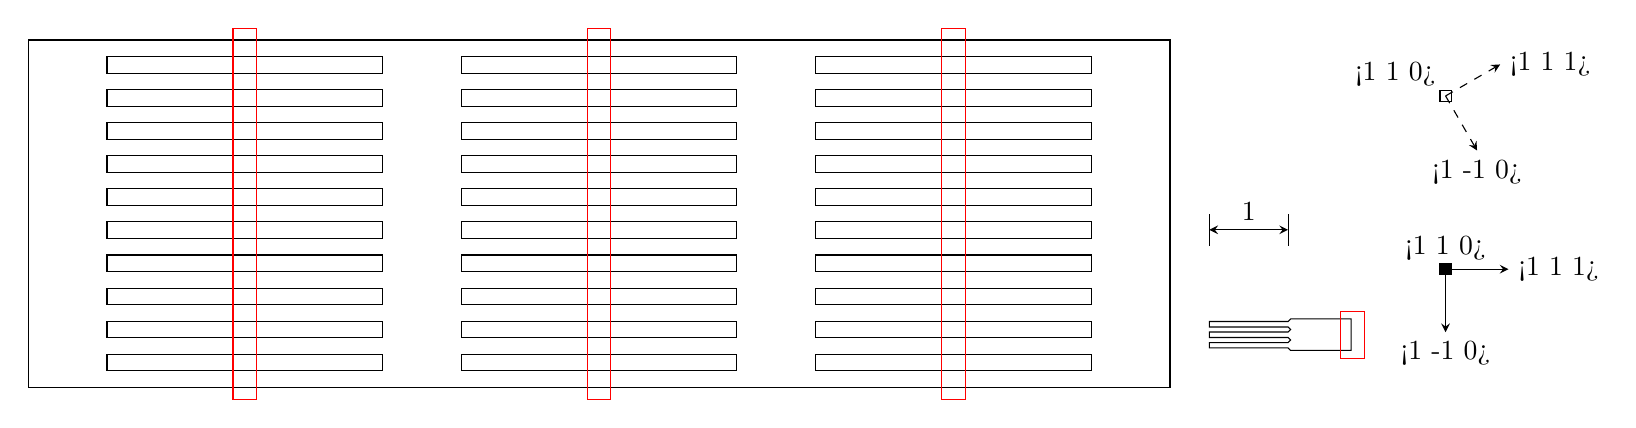
\begin{tikzpicture}
            \begin{scope}
                \draw (0, 0) rectangle (14.5, 4.41);
                \foreach \x in {1, 5.5, 10}
                    \foreach \y in {1, 3, 5, 7, 9, 11, 13, 15, 17, 19}
                        \draw (\x, \y*0.21) rectangle (\x+3.5, 0.21+\y*0.21);
                \foreach \x in {2.6, 7.1, 11.6}
                    \draw [red] (\x, -0.15) rectangle (\x+0.3, 4.56);
            \end{scope}
            \begin{scope}[shift={(15cm, 0.5cm)}]
                \draw (0,0) -- ++ (1, 0) -- ++ (-45:0.045255) -- ++ (0.768, 0) -- ++ (0, 0.4) -- ++ (-0.768, 0) -- ++ (-135:0.045255) -- ++ (-1, 0) -- ++ (0, -0.07) -- ++ (1, 0) -- ++ (-45:0.045255) -- ++ (-135:0.045255) -- ++ (-1, 0) -- ++ (0, -0.07) -- ++ (1, 0) -- ++ (-45:0.045255) -- ++ (-135:0.045255) -- ++ (-1, 0) -- cycle;
                \draw [red] (1.668, -0.132) rectangle (1.968, 0.468);
                \draw[stealth-stealth] (0, 1.5) -- (1, 1.5) node [midway, anchor = south] {\qty{1}{\micro\metre}};
                \draw (0, 1.3) -- (0, 1.7);
                \draw (1, 1.3) -- (1, 1.7);
            \end{scope}
            \begin{scope}[shift={(18cm, 1.5cm)}]
                \draw[-stealth] (0cm, 0cm) -- ++ (-90:0.8cm) node[anchor=north] {\hkl<1 -1 0>};
                \draw[-stealth] (0cm, 0cm)  node[anchor=south] {\hkl<1 1 0>} -- ++ (0:0.8cm) node[anchor=west] {\hkl<1 1 1>};
                \node[mark size=2pt] at (0, 0) {\pgfuseplotmark{square*}};
            \end{scope}
            \begin{scope}[shift={(18cm, 3.7cm)}, rotate=30]
                \draw[-stealth, dashed] (0cm, 0cm) -- ++ (-90:0.8cm) node[anchor=north] {\hkl<1 -1 0>};
                \draw[-stealth, dashed] (0cm, 0cm)  node[anchor=south east] {\hkl<1 1 0>} -- ++ (0:0.8cm) node[anchor=west] {\hkl<1 1 1>};
                \node[mark size=2pt] at (0, 0) {\pgfuseplotmark{square}};
            \end{scope}
        \end{tikzpicture}
    }
    \caption{Microstructure designs for \acs{tase} growth. The structures transferred to the \acs{si} device layer are represented in black and the template opening regions in red. \subref{subfig:110_design1} shows the double comb structures grown on the first \hkl[1 1 0] samples. These were always oriented to have the template axis coincide with the in-plane \hkl<1 1 1> directions. \subref{subfig:110_design2} shows the nanowire array structures used in later experiments on the \hkl[1 1 0] \acs{soi}s and the "merge wire" structures. These types of structures were grown both aligned with the in-plane \hkl[1 1 1] direction, as highlighted by the solid-line arrows, and \qty{30}{\degree} misaligned, as shown by the dashed arrows \cite{Brugnolotto2023_2}.}
    \label{fig:110_Template_Design}
\end{sidewaysfigure}

Figure~\ref{fig:110_Template_Design} shows the evolution of the \acs{tase} structures from those in Figure~\ref{fig:001_Templat5e_Design}. The comb structure of Figure~\ref{subfig:enterprise_design} is perfect for \acf{sem_m} analysis of multiple wires in a single image and the \acf{stem_m} survey of cross-section cuts perpendicular to the growth direction. However, cross-sections parallel to the growth direction only allow for the analysis of a single wire.
\par
As the analysis of heterointerfaces stacked along the growth vector is the primary goal of this work, maximising the number of wires observable from seed to final interface in a single \acf{fib} cut is a key objective of the design phase. Taking inspiration from the "T-shaped" structure in Figure~\ref{subfig:enterprise_design} the first evolution of the comb array is shown in Figure~\ref{subfig:110_design1}. A central rectangular \acs{si} backbone anchors two rows of nanowires that extend from either side, with the templates being open at the very edges of the structure (in red in Figure~\ref{subfig:110_design1}. The length of the nanowire growth area extends up to \qty{7}{\micro\metre} for this design. These long channels (in relation to their \qty{70}{\nano\metre} height) were designed to study the effect of growth in "deep" templates on resulting composition and growth rates. Unfortunately, in practice, the resulting structure could only be used with short etch-back segments. This was due to the thickness of the side walls in the final samples, which was insufficient to ensure structural integrity during \acs{tmah} etch-back, despite the selectivity of this etchant.
\par
The difficulties encountered with the design in Figure~\ref{subfig:110_design1} together with the possibility of having more \acs{stem_m}-observable nanowires per \acs{fib} cut led to the design of the array structure in Figure~\ref{subfig:110_design2}. This allows for the \acs{stem_m} analysis of \num{6} short nanowires up to \qty{2}{\micro\metre}-long while keeping the overall length of the structure at \qty{14.5}{\micro\metre}, and therefore comparable to that of the double-comb design (\qty{13}{\micro\metre}). There are \num{4} equidistant rectangular backbone anchors, with two marking the beginning and end of the structure. The templates are open between the anchors in three areas of the structures (in red in Figure~\ref{subfig:110_design2}). Thus, once complete, one such array contains \num{66} growth sites.

Wire widths of \qty{70}{\nano\metre}, \qty{140}{\nano\metre}, \qty{210}{\nano\metre}, and \qty{280}{\nano\metre} were fabricated, the Figures~\ref{subfig:110_design1} and \ref{subfig:110_design2} show the \qty{210}{\nano\metre} designs.

To the bottom right of the array in Figure~\ref{subfig:110_design2} there is a "merge wire" structure. In this structure, three nucleation wires with a design width of \qty{70}{\nano\metre} all terminate in a single channel \qty{400}{\nano\metre} wide. This structure was designed to study the merging regions between the three growing crystals to observe the defects that could form from the merging of two growing crystals. In the past, it was employed to demonstrate the introduction of dislocations in \acs{tase} microstructures \cite{Mauthe2021}.

Both structures in Figure~\ref{subfig:110_design2} were grown aligned to the in-plane \hkl<1 1 1> direction but also \qty{30}{\degree} misaligned. In practice, this was done by aligning one set of structures to an in-plane \hkl<1 1 1> direction and rotating each subsequent set by \qty{90}{\degree}. Selecting this specific \qty{30}{\degree} misalignment as a basis for analysis therefore has two advantages:
\begin{enumerate}
    \item the resulting seed surfaces and projected growth fronts are at a significant angle with the template sidewalls
    \item there is no need to keep track of the direction of the notch past the dicing stage which resulted in the initial \qtyproduct{6 x 6}{cm} die.
\end{enumerate}

\subsection{\texorpdfstring{\acs{fib} lamella fabrication}{FIB lamella fabrication}}

\begin{figure}
    \centering
    \tikzsetnextfilename{110_FIB}
    \begin{tikzpicture}[isometric]
        \draw (0, 0, 0) -- (0, 0, 2) -- (0, 1, 2) -- (0, 1, 0) -- cycle;
        \draw (0, 0, 0) -- (3, 0, 0) -- (3, 1, 0) -- (0, 1, 0);
        \draw (0, 0, 2) -- (3, 0, 2) -- (3, 1, 2) -- (0, 1, 2);
        \draw (3, 0, 0) -- (3, 0, 2);
        \draw (3, 1, 0) -- (3, 1, 2);
            
        \draw (-0.2, 0, -0.2) -- (-0.2, 0, 2.2) -- (-0.2, 1.2, 2.2) -- (-0.2, 1.2, -0.2) -- cycle;
        \draw (-0.2, 0, -0.2) -- (5, 0, -0.2) -- (5, 1.2, -0.2) -- (-0.2, 1.2, -0.2);
        \draw (-0.2, 0, 2.2) -- (5, 0, 2.2) -- (5, 1.2, 2.2) -- (-0.2, 1.2, 2.2);
        \draw (5, 0, -0.2) -- (5, 0, 2.2);
        \draw (5, 1.2, -0.2) -- (5, 1.2, 2.2);
            
        \path [fill=red!50!, fill opacity=0.3] (-0.5, 0.2, -0.5) -- (-0.5, 0.2, 2.5) -- (5.5, 0.2, 2.5) -- (5.5, 0.2, -0.5) -- cycle;
        \path [fill=red!50!, fill opacity=0.3] (-0.5, 0.8, -0.5) -- (-0.5, 0.8, 2.5) -- (5.5, 0.8, 2.5) -- (5.5, 0.8, -0.5) -- cycle;
            
        \draw [red, dashed] (-0.2, 0.2, -0.2) -- (5, 0.2, -0.2) -- (5, 0.2, 2.2) -- (-0.2, 0.2, 2.2) -- cycle;
        \draw [red, dashed] (-0.2, 0.8, -0.2) -- (5, 0.8, -0.2) -- (5, 0.8, 2.2) -- (-0.2, 0.8, 2.2) -- cycle;

        \begin{scope}[shift={(6, 6, 1)}]
            \draw [-stealth] (0, 0, 0) -- ++ (1, 0, 0) node[anchor = north west]{\hkl<-1 1 1>};
            \draw [-stealth] (0, 0, 0) -- ++ (0, 1, 0) node[anchor = south]{\hkl<1 1 0>};
            \draw [-stealth] (0, 0, 0) -- ++ (0, 0.5, 0.866) node[anchor = east]{\hkl<0 1 -1>};
            \draw [-stealth] (0, 0, 0) -- ++ (0, 0.5, -0.866) node[anchor = south west]{\hkl<1 0 1>};
            \draw [-stealth] (0, 0, 0) -- ++ (0, 0, 1) node[anchor = north east]{\hkl<-1 1 -2>};
        \end{scope}

        \begin{scope}[shift={(10, 5, 0)}]
            \draw (0, 0, 0) -- (0, 0, 2) -- (0, 1, 2) -- (0, 1, 0) -- cycle;
            \draw (0, 0, 0) -- (3, 0, 0) -- (3, 1, 0) -- (0, 1, 0);
            \draw (0, 0, 2) -- (3, 0, 2) -- (3, 1, 2) -- (0, 1, 2);
            \draw (3, 0, 0) -- (3, 0, 2);
            \draw (3, 1, 0) -- (3, 1, 2);
            
            \draw (-0.2, 0, -0.2) -- (-0.2, 0, 2.2) -- (-0.2, 1.2, 2.2) -- (-0.2, 1.2, -0.2) -- cycle;
            \draw (-0.2, 0, -0.2) -- (5, 0, -0.2) -- (5, 1.2, -0.2) -- (-0.2, 1.2, -0.2);
            \draw (-0.2, 0, 2.2) -- (5, 0, 2.2) -- (5, 1.2, 2.2) -- (-0.2, 1.2, 2.2);
            \draw (5, 0, -0.2) -- (5, 0, 2.2);
            \draw (5, 1.2, -0.2) -- (5, 1.2, 2.2);

            \path [fill=red!50!, fill opacity=0.3] (-0.54641016, -0.3, 0.22679492) -- (-0.54641016, 1.5, 1.2660254) -- (5.57735027, 1.5, 1.2660254) -- (5.57735027, -0.3, 0.22679492) -- cycle;
            \path [fill=red!50!, fill opacity=0.3] (-0.54641016, -0.3, 1.12679492) -- (-0.54641016, 1.5, 2.1660254) -- (5.57735027, 1.5, 2.1660254) -- (5.57735027, -0.3, 1.12679492) -- cycle;
        
            \draw [red, dashed] (-0.2, 0, 0.4) -- (5, 0, 0.4) -- (5, 1.2, 1.09282032) -- (-0.2, 1.2, 1.09282032) -- cycle;
            \draw [red, dashed] (-0.2, 0, 1.3) -- (5, 0, 1.3) -- (5, 1.2, 1.99282032) -- (-0.2, 1.2, 1.99282032) -- cycle;
        \end{scope}
    \end{tikzpicture}
    \caption{\acs{fib} cutting strategies to expose \hkl{1 1 0} facets from a \hkl[1 1 0]-oriented substrate. The red-shaded planes show how the cut planes are selected to expose the sides of the wire in correspondence to \hkl{1 1 0} facets if the template axis coincides with a \hkl<1 1 1> direction.}
    \label{fig:110_FIB}
\end{figure}

While a new \hkl<1 1 0> wafer and \hkl<1 1 1> template orientation were used for fabrication, the preference for an exposed \hkl{1 1 0} facet for structural analysis with \acs{stem_m} remains unaltered due to this facet allowing easy recognition of a wide variety of crystalline defects \cite{Dasilva2017}. However, the first difficulty is that, as highlighted in Figure~\ref{subfig:110_etchback}, the in-plane crystalline direction perpendicular to the \hkl<1 1 1> template axis is a \hkl<1 1 2>, making the simple cross-section cut used in the previous chapter (Figure~\ref{subfig:FIB_cut_strategy}) unsuitable.

The most obvious \hkl<1 1 0> direction perpendicular to the \hkl<1 1 1> template axis is the one that defines the wafer orientation itself. As shown on the left of Figure~\ref{fig:110_FIB}, a plane-view cut would satisfy orientation requirements and allow for precise \acf{eds} composition maps and an excellent overview of the evolution of the growth front. However, such a cut is much more complex and time-consuming than a cross-sectional cut. The amount of lamella that must be thinned to sub \qty{100}{\nano\metre} thickness to ensure electron transparency increased from a few hundred nanometres to \qty{1.5}{\micro\metre}, which is challenging to do with the ion beam of the \acs{fib} and requires a high level of precision. This is particularly true when milling both sides of a target region composed of multiple material layers eroded at different rates.

A compromise can be found by cutting the sample with a \qty{30}{\degree} tilt in the stage resulting in the cutting planes drawn on the nanowire on the right in Figure~\ref{fig:110_FIB}. Referring to the direction legend in Figure~\ref{fig:110_FIB}, these expose the \hkl(1 0 1) facet, part of the family of \hkl{1 1 0} facets which all share the same symmetry in the zincblende phase (space group \num{216}) \cite{wyckoff1963crystal, osti_gaas_zb, osti_inas_zb, osti_inp_zb}. This "\qty{30}{\degree} cut" allows an analysis of the evolution of the growth front comparable to the simple cross-section cut used in the previous chapter (Figure~\ref{subfig:FIB_cut_strategy}). Still, tilt means that any material layers not perpendicular to the growth front will appear warped, and, similarly, horizontal and tilted heterointerfaces will be shaded in \acs{eds} analysis. Therefore, a limited use of the regular \qty{90}{\degree} cross section was kept at the beginning for the experiments with the \hkl<1 1 0> wafer.

\section{Application of the growth recipe on the new substrate}

\begin{sidewaysfigure}
    \centering
    \subcaptionbox{
    Growth recipe for sample 4 \cite{Brugnolotto2023}. Each line represents an active flow of the corresponding precursor into the reactor. The colour of the horizontal lines represents the target material. The dashed lines are time-compressed 10 times. The \acl{qw} growth loop was executed three times.
    \label{subfig:recipe4}
    }{
        \tikzsetnextfilename{recipe4}
        \begin{tikzpicture}
        \begin{scope}
        % lines
            \node [label={[label distance=0]180:\acs{in}}] at (0, 0) {};
            \draw [cb1_orange, ultra thick, dashed] (0, 0) -- (2, 0); %/10
            \draw [cb1_dark_blue, ultra thick, dashed] (2, 0) -- (4, 0); %10
            \draw [cb1_orange, ultra thick] (6, 0) -- (8, 0);
            \draw [cb1_dark_blue, ultra thick, dashed] (10, 0) -- (12, 0); %10
        
            \node [label={[label distance=0]180:\acs{ga}}] at (0, -0.5) {};
            \draw [cb1_orange, ultra thick, dashed] (0, -0.5) -- (2, -0.5cm); %/10
            \draw [cb1_orange, ultra thick] (6, -0.5) -- (8, -0.5);
        
            \node [label={[label distance=0]180:\acs{as}}] at (0, -1) {};
            \draw [cb1_orange, ultra thick, dashed] (0, -1) -- (2, -1); %/10
            \draw [cb1_orange, ultra thick] (6, -1) -- (8, -1);
            \draw [gray, ultra thick] (8, -1) -- (9, -1);
        
            \node [label={[label distance=0]180:\acs{p}}] at (0, -1.5) {};
            \draw [cb1_dark_blue, ultra thick, dashed] (2, -1.5) -- (4, -1.5); %/10
            \draw [gray, ultra thick] (4, -1.5) -- (6, -1.5);
            \draw [gray, ultra thick] (9, -1.5) -- (10, -1.5);
            \draw [cb1_dark_blue, ultra thick, dashed] (10, -1.5) -- (12, -1.5); %/10
            \draw [gray, ultra thick] (12, -1.5) -- (14, -1.5);
        
    % labels and markers for the timescale
            \node [label={[label distance=0]180:Time (\second)}] at (0, -2) {};
            \draw [dashed] (0, -2) -- (4, -2);
            \draw [] (4, -2) -- (10, -2);
            \draw [dashed] (10, -2) -- (12, -2);
            \draw [-stealth] (12, -2) -- (14.3, -2); % +0.3
            \draw [] (0, 0.2) -- (0, -2.2) node[anchor = north] {\num{0}};
            \draw [] (2, 0.2) -- (2, -2.2) node[anchor = north] {\num{200}};
            \draw [] (4, 0.2) -- (4, -2.2) node[anchor = north] {\num{400}};
            \draw [] (6, 0.4) -- (6, -2.2) node[anchor = north] {\num{420}};
            \draw [] (8, 0.2) -- (8, -2.2) node[anchor = north] {\num{460}};
            \draw [] (9, 0.2) -- (9, -2.2) node[anchor = north] {\num{470}};
            \draw [] (10, 0.2) -- (10, -2.2) node[anchor = north] {\num{480}};
            \draw [] (12, 0.2) -- (12, -2.2) node[anchor = north] {\num{680}};
            \draw [] (14, 0.4) -- (14, -2.2) node[anchor = north] {\num{700}};
            \draw [stealth - stealth] (6, 0.3) -- (14, 0.3) node[midway, anchor=south] {Quantum Well Loop (x\num{3})};
        \end{scope}
        \begin{scope} [shift={(15.2cm, -0.5)}] % +0.9
            \draw [gray, ultra thick] (0, 0.5) -- (0.5, 0.5) node[anchor = west, text=black] {Hold Step};
            \draw [cb1_orange, ultra thick] (0, 0) -- (0.5, 0) node[anchor = west, text=black] {\acs{ingaas}};
            \draw [cb1_dark_blue, ultra thick] (0, -0.5) -- (0.5, -0.5) node[anchor = west, text = black] {\acs{inp}};
            \draw [dashed, ultra thick] (0, -1) -- (0.5, -1) node[anchor = west, text = black] {\num{0.1} time scale};
            \draw (-0.3, 1) -- (3.3, 1) -- (3.3, -1.65) -- node[midway, fill = white] {Legend} (-0.3, -1.65) -- cycle;
        \end{scope}
        \end{tikzpicture}
    }
    \subcaptionbox{
    \acs{bf}-\acs{stem_m} overview images of two nanowires from sample 4. The wire on the left was cut with a regular cross-section, while the wire on the right was cut with a \qty{30}{\degree} cross-section.
    \label{subfig:s4_OV}
    }{
    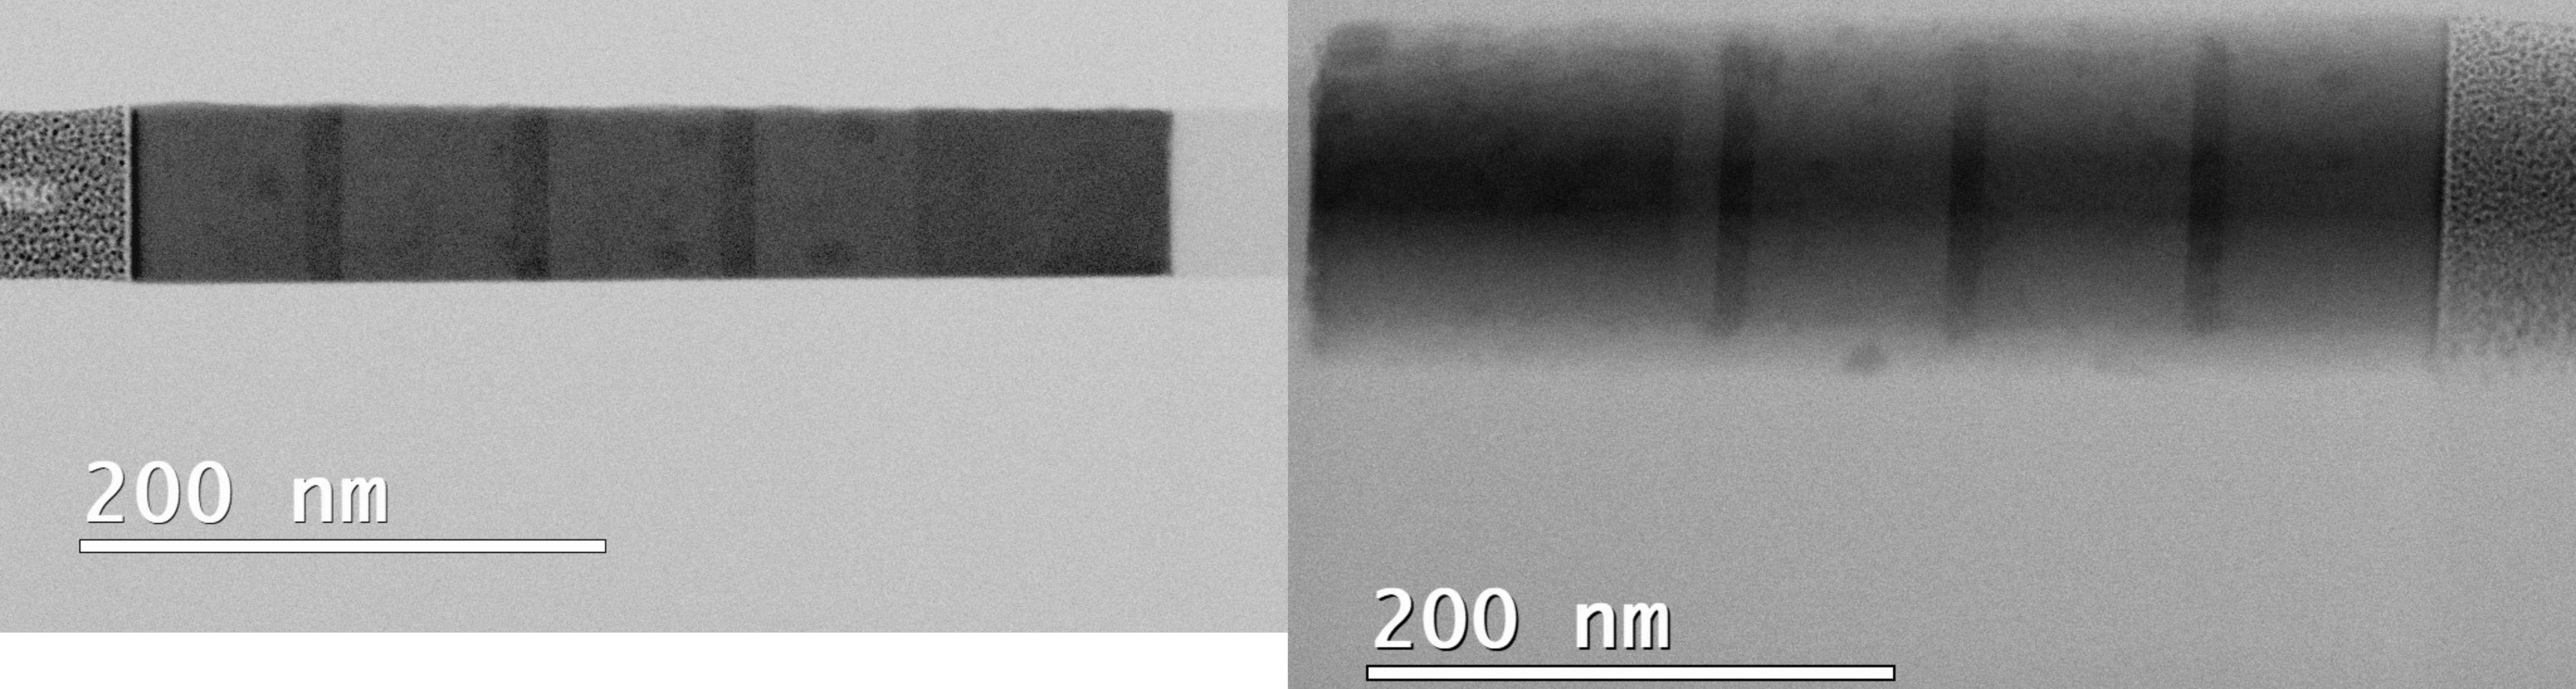
\includegraphics[width = 0.48\textwidth]{4_Properties/Fig/s4_OV.pdf}
    }
    \subcaptionbox{
    High-resolution \acs{bf}-\acs{stem_m} images of the first \acl{qw} for both wires in \subref{subfig:s4_OV} with \acs{fft} inserts.
    \label{subfig:s4_HR}
    }{
    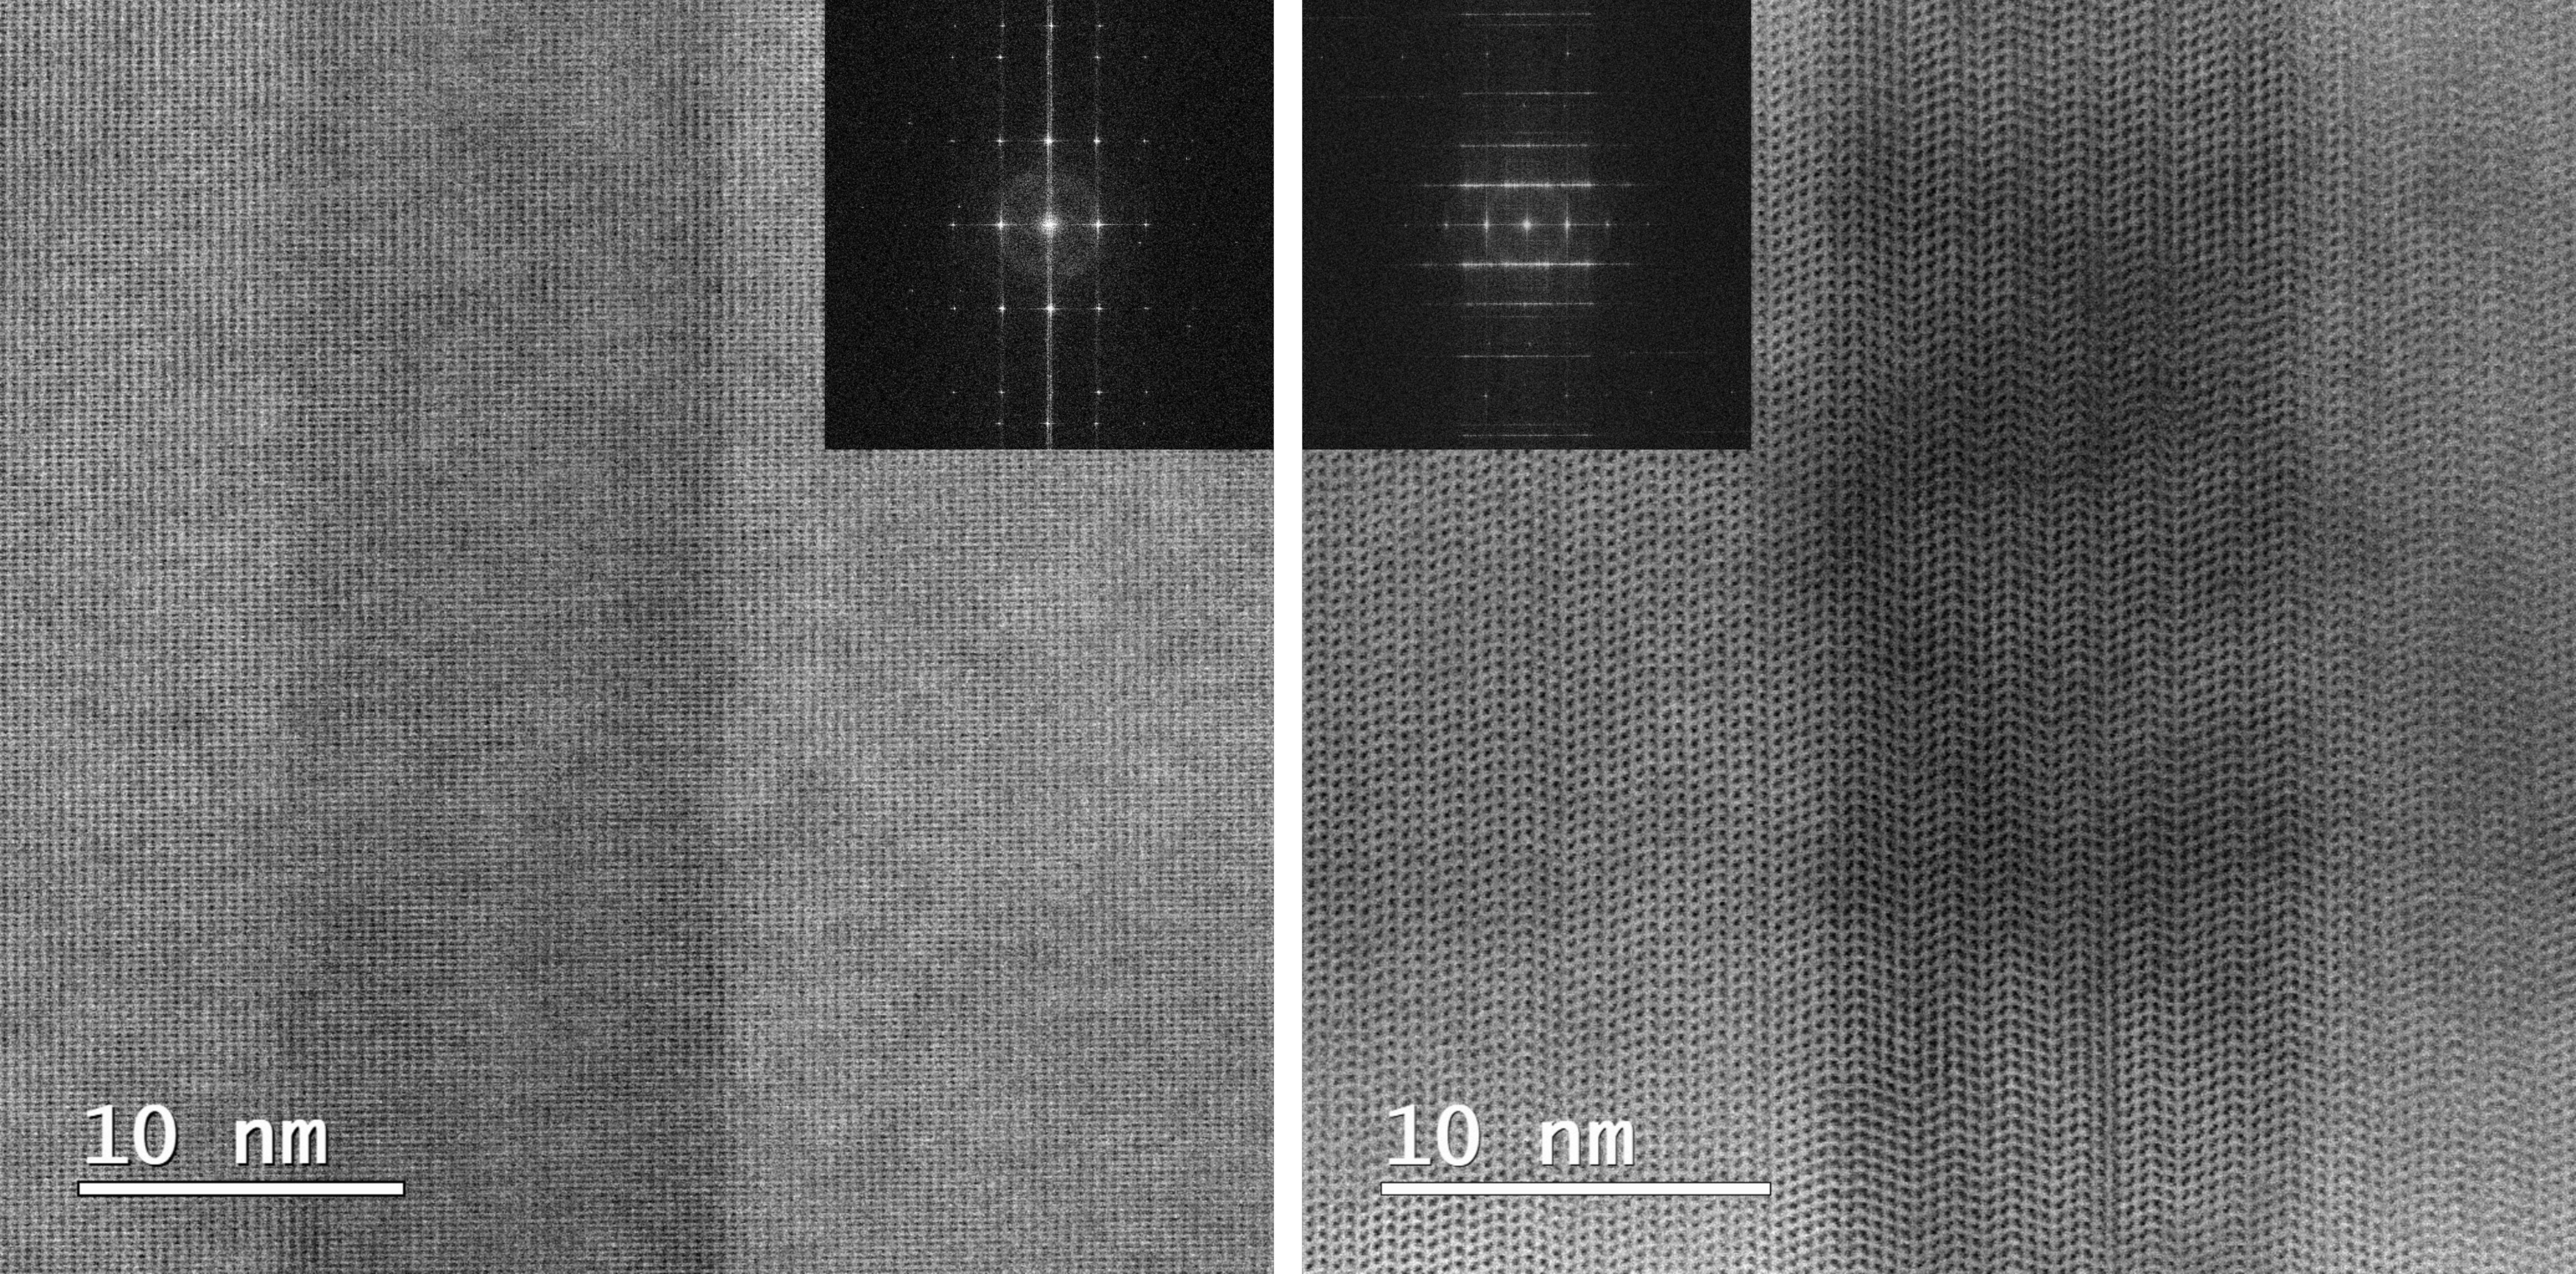
\includegraphics[width = 0.48\textwidth]{4_Properties/Fig/s4_HR.pdf}
    }
    \caption{Growth recipe and \acs{bf}-\acs{stem_m} images of sample 4. The III-V material appears dark due to channelling contrast, with \acs{ingaas} being the darkest of the two III-V materials. \subref{subfig:recipe4} shows the growth recipe. \subref{subfig:s4_OV} shows overview images of the normal cross-section and \qty{30}{\degree} cross-section. \subref{subfig:s4_HR} shows high-resolution images of the first \acl{qw} for both wires in \subref{subfig:s4_OV} with inserts showing the calculated \acs{fft}s}
    \label{fig:s4_recipe_STEM}
\end{sidewaysfigure}

The recipe in Figure~\ref{subfig:recipe4} was kept similar to that used in sample 3 (Figure~\ref{subfig:recipe3}) for the initial experiment on the new \hkl<1 1 0> substrate. It contains a looped segment for creating \acs{ingaas} \acl{qw}s between \acs{inp} barrier layers. The main adjustments concern the deposition times. The initial growth steps, were changed from \qty{480}{\second} and \qty{180}{\second} to \qty{200}{\second} for both \acs{ingaas} and \acs{inp}, respectively. The deposition times for \acs{ingaas} \acl{qw}s were lowered from \qty{30}{\second} to \qty{20}{\second} in anticipation of the smaller area of the growth front. Simultaneously, the duration of \acs{inp} barrier steps was increased from \qty{180}{\second} to \qty{200}{\second}.

The most significant change concerned the post-\acs{ingaas} hold step. Here, \acs{as} precursor flow step time was reduced from \qty{15}{s} to \qty{10}{s} and the following \acs{p} precursor flow step time increased from \qty{5}{s} to \qty{10}{s}. This change was made to address the \acs{as} profile seen in the \acs{inp} layer of the sample 3 (Figure~\ref{subfig:s3_V_linesc}). By reducing the \acs{as} precursor flow time in the hold step it was hoped that the \acs{as} contamination in the first nanometres of the \acs{inp} layer would be reduced or, in the best case, eliminated in sample 4.

\subsection{Structural Analysis}

Figure~\ref{fig:s4_recipe_STEM} shows \acs{bf}-\acs{stem_m} images of two different wires from sample 4. The images on the left side of both Figure~\ref{subfig:s4_OV} and \ref{subfig:s4_HR} show the wire cut with a standard cross-section used in the previous chapter and schematised in Figure~\ref{subfig:FIB_cut_strategy}. In comparison, on the right side of the same figures, the images of a lamella cut with the \qty{30}{\degree} cross-section illustrated on the right of Figure~\ref{fig:110_FIB} are shown. 

Both lamellae come from the same sample, with identical device layer thickness. 
However, Figure~\ref{subfig:s4_OV} highlights how the \qty{30}{\degree} cross-section appears larger because the viewing angle is not perpendicular to the heterointerfaces that lay in the wafer plane. This distortion becomes clear when one looks at the III-V-\acs{si} interfaces at the top and bottom of the nanowires. The well-defined lines in the standard cross-section become large regions in the \qty{30}{\degree} cross-section. In these regions, the III-V nanowire and the \acs{sio2} template appear superimposed, as they are one on top of the other in the path the electron beam takes through the lamella.

An evident advantage of the \qty{30}{\degree} cut in combination with the \hkl<1 1 0> wafer is that vertical \hkl{1 1 1} heterointerfaces remain perpendicular to the viewing direction. As the recipe optimised in Chapter~\ref{chap:growth} stabilises this facet family, this new viewing angle does not affect the observer's ability to evaluate the sharpness of this type of interface from \acs{stem_m} measurements.

The comparison between the two wires at high resolution in Figure~\ref{subfig:s4_HR} also highlights the amount of structural information available when viewing a \hkl{1 1 0} plane (on the right) compared to a \hkl{1 1 2} plane (on the left). The presence of \acl{rtp}s (\acs{rtp}s) is evident in the \qty{30}{\degree} cross-section both in the \acs{bf}-\acs{stem_m} image and in its \acf{fft} in the insert. The \acs{rtp}s have manifested as horizontal lines in the frequency domain. In contrast, both the \hkl{1 1 2} \acs{bf}-\acs{stem_m} image and its \acf{fft} do not contain any trace of this type of defect.

Both samples grew from \acl{si} seeds that appear (in print) towards the centre of the image and grew out toward the margins. The initial \acs{ingaas} nucleation layer gives way to a lighter \acs{inp} layer in both lamellae, however, the length of this layer appears different. This could be due to a different shape of the nucleation \acs{ingaas}'s growth front. A trace of the complexity of this interface is seen at the bottom of the first well of the \qty{30}{\degree} cross-section. The bottom of this heterostructure appears bent towards the seed, suggesting that the \acs{inp} layer did not have enough time to grow to annihilate all the non-\hkl{1 1 1} facets.

\sisetup{detect-all = true}
\begin{table}[]
    \centering
    \caption{Growth rates for each heterolayer in the two nanowires in Figure~\ref{fig:s4_recipe_STEM}}.
    \begin{tabular}{l|c c}
         & \multicolumn{2}{c}{growth rates (\nmmin)} \\
        material layer & \qty{0}{\degree} cross-section & \qty{30}{\degree} cross-section \\ \hline
        \acs{ingaas} nucleation & \num[separate-uncertainty=true]{29.0 (0.2)} & \num[separate-uncertainty=true]{42.4 (0.3)} \\
        \acs{inp} stabilisation & \num[separate-uncertainty=true]{18.3 (0.1)} & \num[separate-uncertainty=true]{4.7 (0.2)} \\ \hline
        \textbf{pre-wells layers} & \textbf{\num[separate-uncertainty=true]{23.7 (0.1)}} & \textbf{\num[separate-uncertainty=true]{23.6 (0.3)}} \\ \hline
        \acs{ingaas} well 1 & \num[separate-uncertainty=true]{39 (1)} & \num[separate-uncertainty=true]{35 (2)} \\
        \acs{inp} barrier 1 & \num[separate-uncertainty=true]{19.7 (0.2)} & \num[separate-uncertainty=true]{22.4 (0.1)} \\
        \acs{ingaas} well 2 & \num[separate-uncertainty=true]{41 (1)} & \num[separate-uncertainty=true]{38 (1)} \\
        \acs{inp} barrier 2 & \num[separate-uncertainty=true]{19.7 (0.2)} & \num[separate-uncertainty=true]{23.6 (0.1)} \\
        \acs{ingaas} well 3 & \num[separate-uncertainty=true]{43 (1)} & \num[separate-uncertainty=true]{39.1 (0.9)} \\
        \acs{inp} barrier 3 & \num[separate-uncertainty=true]{20.0 (0.2)} & \num[separate-uncertainty=true]{25.0 (0.1)} \\ \hline
        \textbf{wire total} & \textbf{\num[separate-uncertainty=true]{22.5 (0.2)}} & \textbf{\num[separate-uncertainty=true]{24.4 (0.2)}} \\ \hline \hline
    \end{tabular}
    \label{tab:s4_growth_rates}
\end{table}
\sisetup{detect-all = false}

\paragraph{Growth rates} The growth rates for each material layer in the wires of Figure~\ref{fig:s4_recipe_STEM} are summarised in Table~\ref{tab:s4_growth_rates}. These values were calculated by taking seven repeated measurements of each layer thickness perpendicularly to each heterointerface and are therefore comparable to the \hkl{1 1 1} growth rates of sample 3 (Table~\ref{tab:sample3_growth_rates}).

The discrepancy between the size of the \acs{ingaas} and \acs{inp} pre-well layers noted in the \acs{bf}-\acs{stem_m} images of the two wires from sample 4 is also reflected in their growth rates. The \acs{ingaas} growth rate for the nanowire observed with a \qty{30}{\degree} cross-section is \qty[separate-uncertainty=true]{42.4 (0.3)}{\nano\metre\per\minute}: significantly higher than that of its counterpart in the nanowire observed under the standard cross-section which stands at \qty[separate-uncertainty=true]{29.0 (0.2)}{\nano\metre\per\minute}. The \acs{inp} growth rates, however, have an opposite trend, resulting at \qty[separate-uncertainty=true]{4.7 (0.2)}{\nano\metre\per\minute} and \qty[separate-uncertainty=true]{18.3 (0.1)}{\nano\metre\per\minute}, respectively. 

Consequently, when examining the total growth rate of the nanowires before the first \acl{qw} the two values are within each other's error at \qty[separate-uncertainty=true]{23.6 (0.3)}{\nano\metre\per\minute} and \qty[separate-uncertainty=true]{23.7 (0.1)}{\nano\metre\per\minute}, respectively. Since the amount of material introduced in the reactor was the same for both wires, this would support the theory that a complex growth front forms in one of the two wires and then is simplified to a single \hkl{1 1 1} facet by the \acs{inp} layer. In this scenario \acs{inp} and \acs{ingaas} layers could be one behind the other in the path of the electron beam. Another option is that the "missing" \acs{inp} could have been removed during the \acs{fib} thinning of the lamella. During this process, part of the nanowire's material is removed; therefore, the III-V semiconductor film seen in the \acs{stem_m} image is only a portion of the entire wire.

Both the \acs{ingaas} well and \acs{inp} growth rates increase as the growth front approaches the opening of the template. This trend is not very pronounced for the \acs{inp} layers of the nanowire cut with the standard cross-section procedure but is more pronounced in the \qty{30}{\degree} cross-section sample. This results in a higher total growth rate for the latter nanowire, with nearly \qty{2}{\nano\metre\per\minute} of difference. This difference, which develops in the latter precursor-switching-rich part of the recipe when the growth front is nearer to the template opening, could indicate a limited competition between neighbouring nanowires or a precursor concentration gradient in the reactor in the moments immediately following the precursor switches.
\par

\subsection{Compositional analysis}

\begin{figure}
    \centering
    \subcaptionbox{
        III-element \acs{eds} map. Red \acs{in}, blue \acs{ga}
        \label{subfig:s4_0deg_IIImap_wells}
        }{
        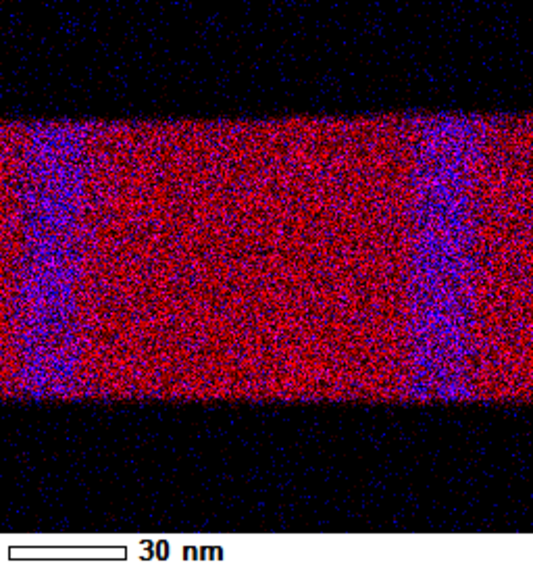
\includegraphics[width=0.48\textwidth]{4_Properties/Fig/s4_0deg_IIImap_wells.pdf}
    }
    \subcaptionbox{
        V-element \acs{eds} map. Red \acs{as}, blue \acs{p}
        \label{subfig:s4_0deg_Vmap_wells}
        }{
        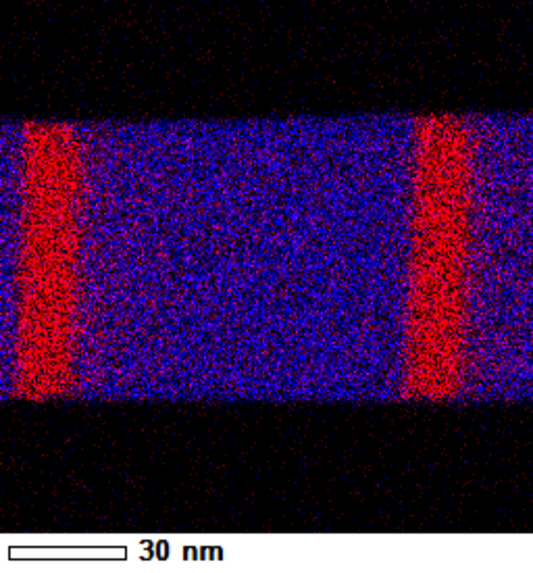
\includegraphics[width=0.48\textwidth]{4_Properties/Fig/s4_0deg_Vmap_wells.pdf}
    }
    \caption{\acs{eds} maps of the \acl{qw} region of the \qty{0}{\degree} sample in Figure~\ref{subfig:s4_OV}. The seed is out of frame on the left of the images.}
    \label{fig:s4_0deg_EDS_maps_wells}
\end{figure}

Figure~\ref{fig:s4_0deg_EDS_maps_wells} shows the \acs{eds} maps. The elements \acl{ga} and \acl{p} are colour-coded in blue while \acl{in} and \acl{as} are colour-coded in red. Two \acs{ingaas} \acl{qw}s are visible on both maps, showing the same nanowire area. 

The III-element map shows how \acl{ga} is well-segregated into the \acs{ingaas} layers. However, a difference between the leading and trailing edges of the \acl{qw}s is visible once more when examining the V-element map. Indeed, while the leading edge is sharp, a light red shading is present in the \acl{p} region after the trailing edge. This indicates an \acl{as} contamination in the \acs{inp} barrier layer. As the image is comparable to the one in Figure~\ref{subfig:s3_V_map_wells}, the lengthening of the \acs{p} flow step during the post \acs{ingaas} hold step had a small impact on the resulting post-well composition profile.

\begin{figure}
    \centering
    \subcaptionbox{
    \acs{eds} linescan: III atomic percentage vs position.
    \label{subfig:s4_III_0deg_linesc}
    }{
    \tikzsetnextfilename{s4_III_0deg_linesc}
    \begin{tikzpicture}
        \begin{axis}[
            width = 0.8\textwidth,
            height = 5cm,
            xlabel = Position (nm),
            ylabel = Composition (atomic \%),
            table/col sep=comma,
            %title = III element composition,
            legend pos=outer north east,
            ymin=0, ymax=100,
            xmin = 0, xmax=230
        ]
    \addplot [cb1_orange,] table[x=nm,y=Ga] {4_Properties/csv/s4_III_0deg_linesc.csv};
    \addplot [cb1_dark_blue,] table[x=nm,y=In] {4_Properties/csv/s4_III_0deg_linesc.csv};
    \addlegendentry{Ga}
    \addlegendentry{In}
    \end{axis}

    \end{tikzpicture}
    }
    \subcaptionbox{
    \acs{eds} linescan: V atomic percentage vs position.
    \label{subfig:s4_V_0deg_linesc}
    }{
    \tikzsetnextfilename{s4_V_0deg_linesc}
    \begin{tikzpicture}
        \begin{axis}[
            width = 0.8\textwidth,
            height = 5cm,
            xlabel = Position (nm),
            ylabel = Composition (atomic \%),
            table/col sep=comma,
            %title = V element composition,
            legend pos=outer north east,
            ymin=0, ymax=100,
            xmin = 0, xmax=230
        ]
    \addplot [cb1_orange,] table[x=nm,y=As] {4_Properties/csv/s4_V_0deg_linesc.csv};
    \addplot [cb1_dark_blue,] table[x=nm,y=P] {4_Properties/csv/s4_V_0deg_linesc.csv};
    \addlegendentry{As}
    \addlegendentry{P}
    \end{axis}

    \end{tikzpicture}
    }
    \caption{\acs{eds} linescan compositional data (in percentage) for the \subref{subfig:s4_III_0deg_linesc} III elements and \subref{subfig:s4_V_0deg_linesc} V elements across all three \acl{qw} of the \qty{0}{\degree} sample seen in Figure~\ref{subfig:s4_OV}. The origin of the x-axis is situated before the first well and is the closest point to the \acs{si} seed. Higher position numbers (in nm) represent the scan moving along the \hkl{1 1 1} vector perpendicular to the growth front away from the seed.}
    \label{fig:s4_0deg_linescans}
\end{figure}

Figure~\ref{fig:s4_0deg_linescans} shows the composition data calculated from the \acs{eds} linescan taken on the \acl{qw} region of the \qty{0}{\degree} sample in Figure~\ref{subfig:s4_OV}. The scan was taken from before the first \acl{qw}, closest to the \acs{si} seed.

The III-element composition profile of Figure~\ref{subfig:s4_III_0deg_linesc} was calculated using the L\(_\alpha\) lines of \acl{in} and \acl{ga}. The graph is very noisy, with noise fluctuations reaching \qty{20}{\%}, but shows a composition close to \ce{In0_.4Ga0_.6As} in all three \acl{qw}s. Similarly to the profile in Figure~\ref{subfig:s3_III_linesc}, suggests the presence of a \acl{ga} composition gradient after the well itself. 

The V-element composition profile of Figure~\ref{subfig:s4_V_0deg_linesc} was calculated using the K\(_\alpha\) lines of \acl{as} and \acl{p}. This graph has noise fluctuations of about \num{10}-\qty{15}{\%}. A \acl{as} percentage composition close to \qty{100}{\%} is present in the \acs{ingaas} \acl{qw} similarly to what was observed for sample 3 (Figure~\ref{subfig:s3_V_linesc}). The \acs{as}-rich region extends for \num{10}-\qty{15}{\nano\metre} after the end of the \acs{ingaas} \acl{qw}.

As the precursor flows were not altered from those of previous samples, the V / III ratios remain as in Table~\ref{tab:sample1_ratios}. The higher concentration of \acl{ga} in the \acl{qw}s could therefore be caused by the change in the geometry of the template given by the difference in device layer thickness of the \hkl<1 1 0> \acs{soi} wafer.

\subsection{Photoluminescence analysis}

\begin{figure}
    \centering
    \tikzsetnextfilename{s4_pl}
    \begin{tikzpicture}
        \begin{axis}[
            width = 0.8\textwidth,
            height = 5cm,
            xlabel = Wavelegth (nm),
            ylabel = Intensity (a.u.),
            table/col sep=comma,
            %title = Photoluminescence Spectrum,
            legend pos=outer north east,
            ymin=0, ymax=1000,
            xmin = 1268.8, xmax=1600.3
            ]
            \addplot [cb1_dark_blue,] table[x=wavelength,y=intensity] {4_Properties/csv/s4_pl.csv};
            \addlegendentry{Sample 4}
        \end{axis}
    \end{tikzpicture}
    \caption{Photoluminescence spectrum of a nanowire from sample 4. This spectrum was kindly recorded by Markus Scherrer.}
    \label{fig:s4_pl}
\end{figure}

The photoluminescence spectrum in Figure~\ref{fig:s4_pl} was recorded from one of the nanowires in sample 4. The operator selected a nanowire far from parasitic growths. The nanowire was excited with a \qty{1}{\second}-long laser pulse with a wavelength of \qty{1000}{\nano\metre} while cooled to \qty{-200}{\kelvin}. This wavelength was selected as it is higher than the absorption wavelength of \acs{inp} (\qty{920}{\nano\metre} \cite{Bachmann1981}) but lower than that of \ce{In0_.53Ga0_.47As} (\qty{1650}{\nano\metre} \cite{Takeda1976}) in order to selectively excite the latter material. 

As the focus size of a wave is limited by both the diffraction limit and the real (therefore imperfect) optics of the setup, the illumination spot used to excite the nanowire is larger than \qty{500}{\nano\metre} and can be approximated at an order of magnitude of \qty{1}{\micro\metre} \cite{Scherrer2021}. As such, the spot size is much larger than that of even just one of the nanowires, let alone that of the single heterolayers. 

One of the nanowires at the edge of one of the comb structures shown in Figure~\ref{subfig:110_design1} was chosen for measurement to minimise the influence of neighbouring wires as much as possible. The resulting spectrum of Figure~\ref{fig:s4_pl} shows a wide emission range, with an emission peak at the edge of the detector cutoff. The reason for this wide spectrum could lie in the large \acs{ingaas} nucleation layer, which still constitutes the bulk of \acs{ingaas} in the nanowire and grows before the facet stabilisation process mediated by the following \acs{inp} layer.

As such, it becomes important to minimise the length of this nucleation layer as much as possible if the photoluminescence spectrum of the \acs{ingaas} heterostructures is to be recorded.

\section{Minimisation of Nucleation Layer Thickness}

\begin{sidewaysfigure}
    \centering
    \subcaptionbox{
    Growth recipe for sample 5 and for merge structures \cite{Brugnolotto2023_2}. Each line represents an active flow of the corresponding precursor into the reactor. The colour of the horizontal lines represents the target material. The dashed lines are time-compressed 10 times. The \acl{qw} growth loop was executed three times.
    \label{subfig:recipe5}
    }{
        \tikzsetnextfilename{recipe5}
        \begin{tikzpicture}
        \begin{scope}
        % lines
            \node [label={[label distance=0]180:\acs{in}}] at (0, 0) {};
            \draw [cb1_orange, ultra thick] (0, 0) -- (3, 0); 
            \draw [cb1_dark_blue, ultra thick, dashed] (3, 0) -- (7.5, 0); %10
            \draw [cb1_orange, ultra thick] (9.5, 0) -- (10.5, 0);
            \draw [cb1_dark_blue, ultra thick, dashed] (12.5, 0) -- (14.5, 0); %10
        
            \node [label={[label distance=0]180:\acs{ga}}] at (0, -0.5) {};
            \draw [cb1_orange, ultra thick] (0, -0.5) -- (3, -0.5cm); 
            \draw [cb1_orange, ultra thick] (9.5, -0.5) -- (10.5, -0.5);
        
            \node [label={[label distance=0]180:\acs{as}}] at (0, -1) {};
            \draw [cb1_orange, ultra thick] (0, -1) -- (3, -1); 
            \draw [cb1_orange, ultra thick] (9.5, -1) -- (10.5, -1);
            \draw [gray, ultra thick] (10.5, -1) -- (11.5, -1);
        
            \node [label={[label distance=0]180:\acs{p}}] at (0, -1.5) {};
            \draw [cb1_dark_blue, ultra thick, dashed] (3, -1.5) -- (7.5, -1.5); %/10
            \draw [gray, ultra thick] (7.5, -1.5) -- (9.5, -1.5);
            \draw [gray, ultra thick] (11.5, -1.5) -- (12.5, -1.5);
            \draw [cb1_dark_blue, ultra thick, dashed] (12.5, -1.5) -- (14.5, -1.5); %/10
            \draw [gray, ultra thick] (14.5, -1.5) -- (16.5, -1.5);
        
    % labels and markers for the timescale
            \node [label={[label distance=0]180:Time (\second)}] at (0, -2) {};
            \draw [] (0, -2) -- (3, -2);
            \draw [dashed] (3, -2) -- (7.5, -2);
            \draw [] (7.5, -2) -- (12.5, -2);
            \draw [dashed] (12.5, -2) -- (14.5, -2);
            \draw [-stealth] (14.5, -2) -- (16.8, -2); % +0.3
            \draw [] (0, 0.2) -- (0, -2.2) node[anchor = north] {\num{0}};
            \draw [] (3, 0.2) -- (3, -2.2) node[anchor = north] {\num{30}};
            \draw [] (7.5, 0.2) -- (7.5, -2.2) node[anchor = north] {\num{480}};
            \draw [] (9.5, 0.4) -- (9.5, -2.2) node[anchor = north] {\num{500}};
            \draw [] (10.5, 0.2) -- (10.5, -2.2) node[anchor = north] {\num{510}};
            \draw [] (11.5, 0.2) -- (11.5, -2.2) node[anchor = north] {\num{520}};
            \draw [] (12.5, 0.2) -- (12.5, -2.2) node[anchor = north] {\num{530}};
            \draw [] (14.5, 0.2) -- (14.5, -2.2) node[anchor = north] {\num{730}};
            \draw [] (16.5, 0.4) -- (16.5, -2.2) node[anchor = north] {\num{750}};
            \draw [stealth - stealth] (9.5, 0.3) -- (16.5, 0.3) node[midway, anchor=south] {Quantum Well Loop (x\num{3})};
        \end{scope}
        \begin{scope} [shift={(17.6cm, -0.5)}] % +0.9
            \draw [gray, ultra thick] (0, 0.5) -- (0.5, 0.5) node[anchor = west, text=black] {Hold Step};
            \draw [cb1_orange, ultra thick] (0, 0) -- (0.5, 0) node[anchor = west, text=black] {\acs{ingaas}};
            \draw [cb1_dark_blue, ultra thick] (0, -0.5) -- (0.5, -0.5) node[anchor = west, text = black] {\acs{inp}};
            \draw [dashed, ultra thick] (0, -1) -- (0.5, -1) node[anchor = west, text = black] {\num{0.1} time scale};
            \draw (-0.3, 1) -- (3.3, 1) -- (3.3, -1.65) -- node[midway, fill = white] {Legend} (-0.3, -1.65) -- cycle;
        \end{scope}
        \end{tikzpicture}
    }
    \subcaptionbox{
    \acs{sem_m} image of nanowire array made with the design in Figure~\ref{subfig:110_design2}.
    \label{subfig:SEM_array}
    }{
    \tikzsetnextfilename{SEM_array}
    \begin{tikzpicture}
        \node[inner sep=0pt] (image) at (0,0) {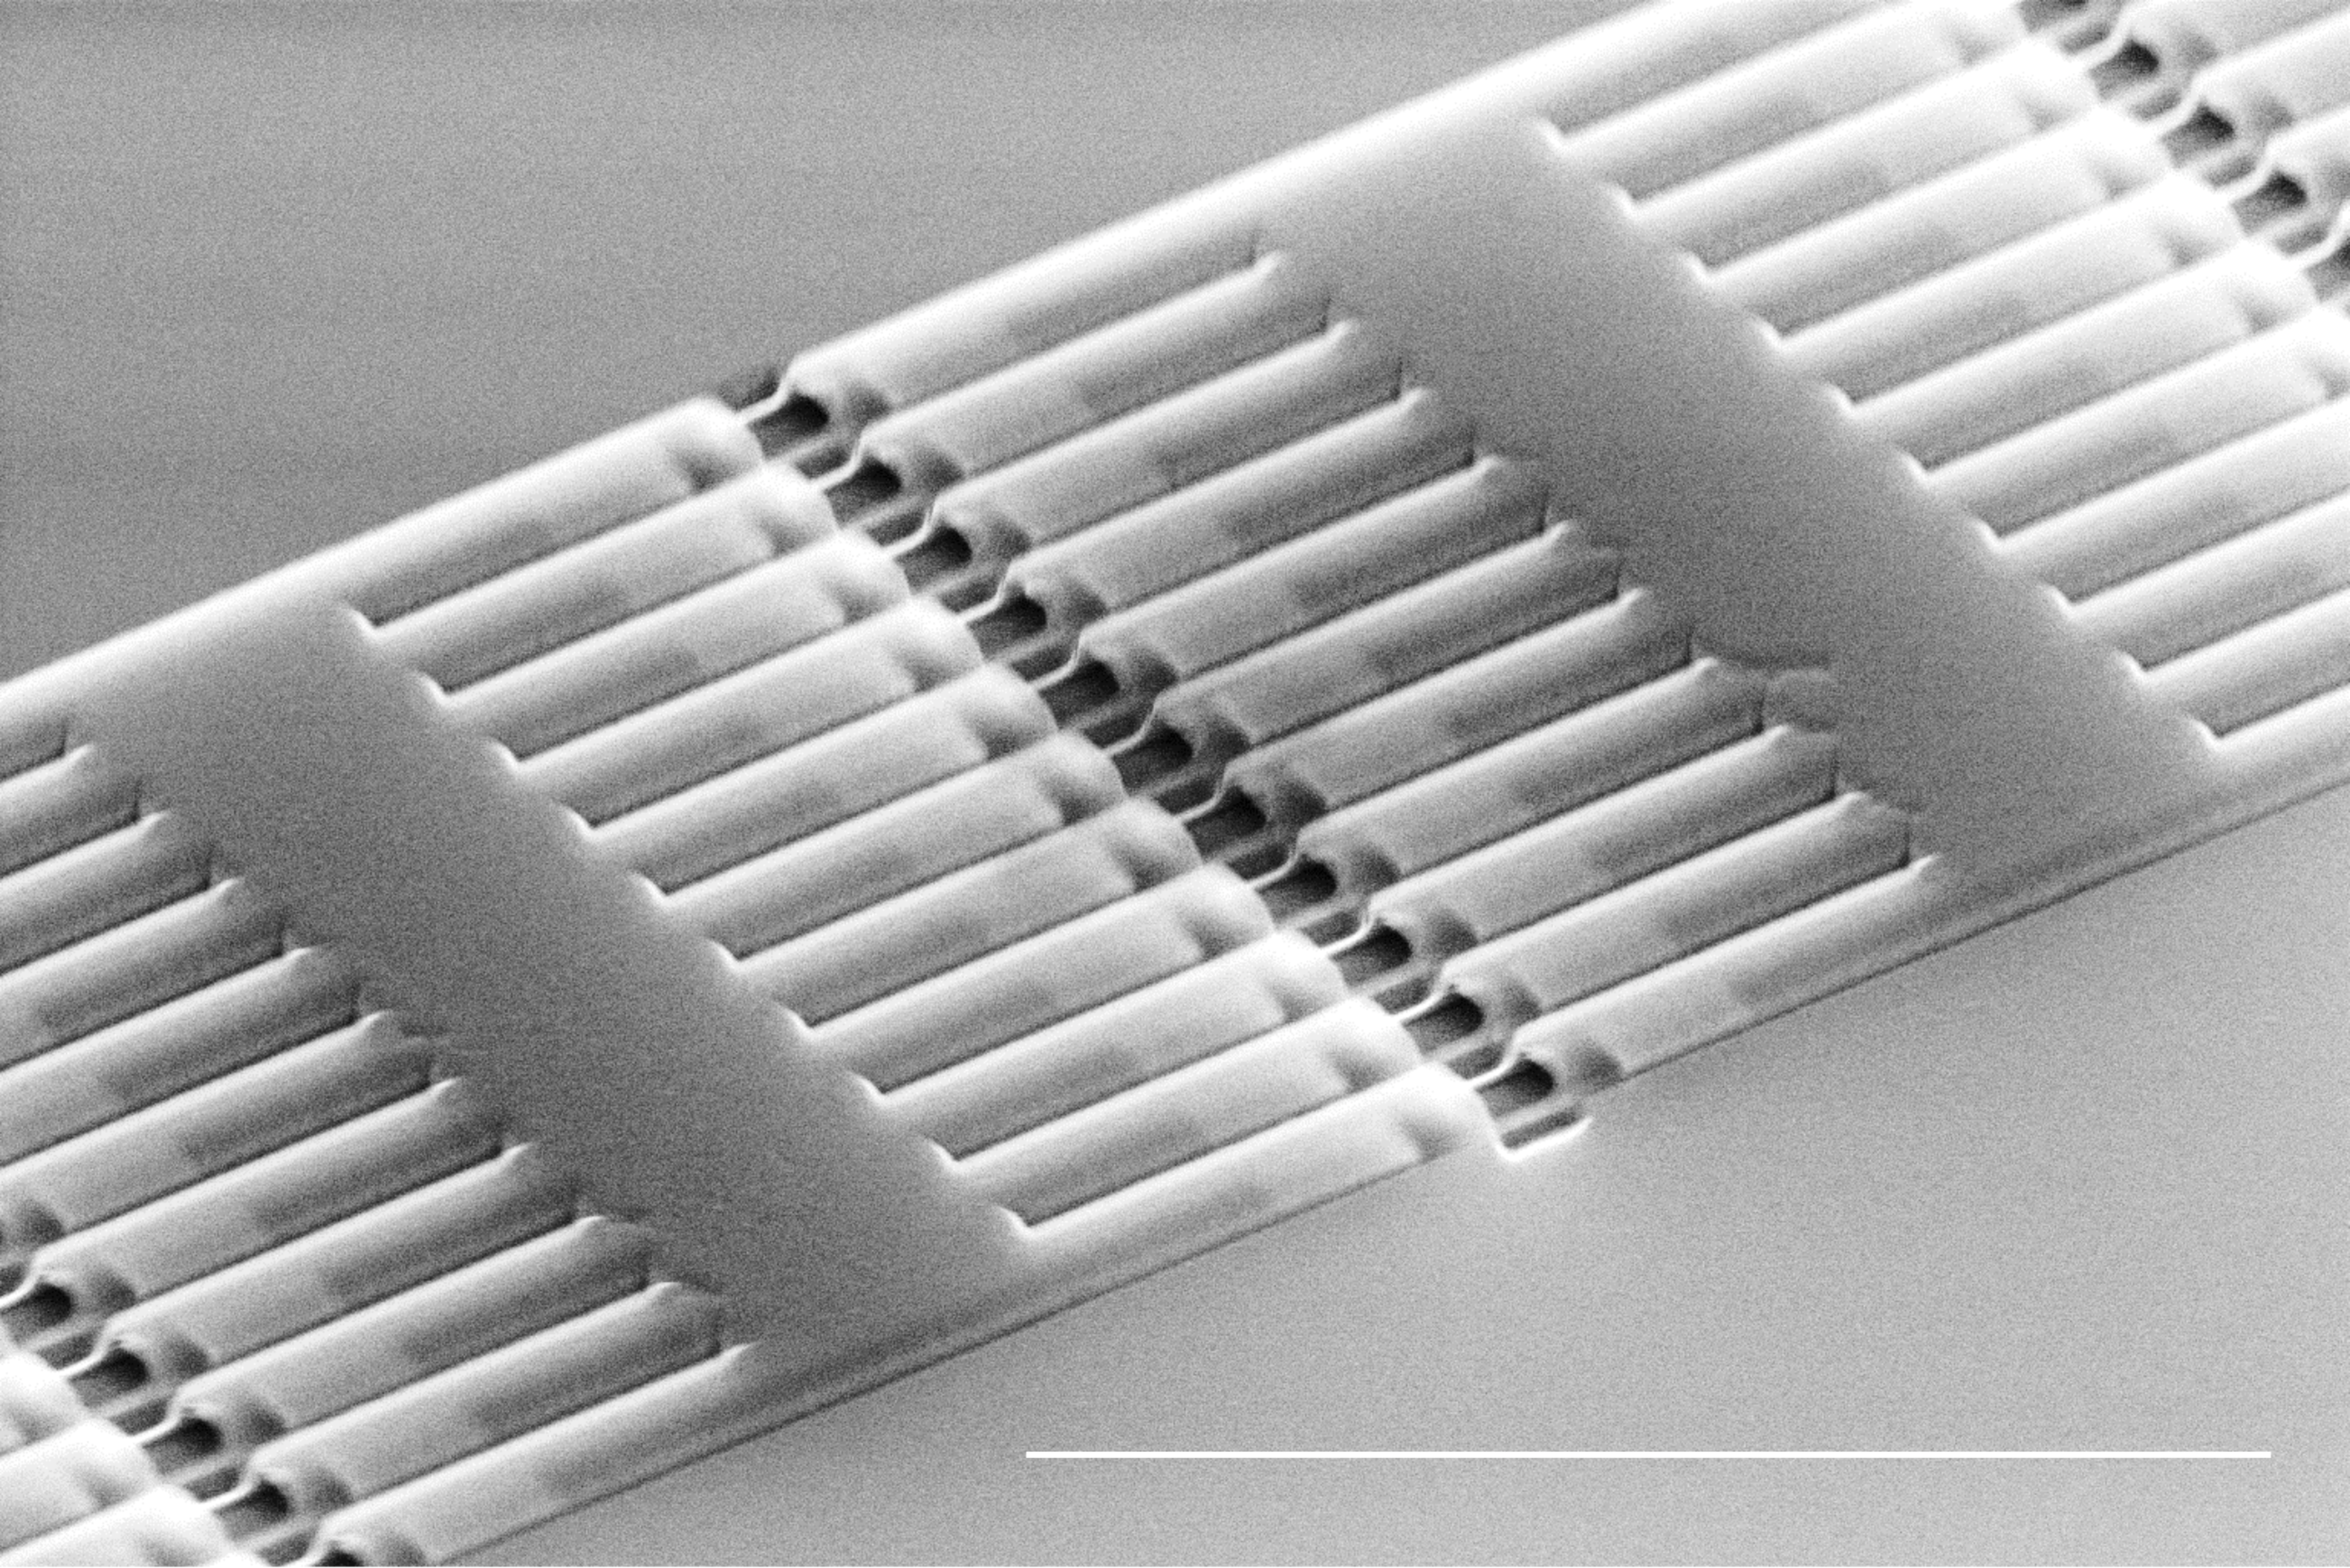
\includegraphics[width = 0.48\textwidth]{4_Properties/Fig/SEM_array.pdf}};
        \node [white] at (5, -3) {\qty{4}{\micro\metre}};
        \node [white, rotate=24] at (-4, 1.6) {\acs{si}};
        \node [white, rotate=24] at (-3.1, 1.9) {III-V};
        \node [white, rotate=-50] at (1.9, -2.5) {Template};
        \node [white, rotate=-50] at (2.4, -2.4) {Opening};
    \end{tikzpicture}
    }
    \subcaptionbox{
    \acs{bf}-\acs{stem_m} overview image of a nanowire from sample 5.
    \label{subfig:s5_OV}
    }{
    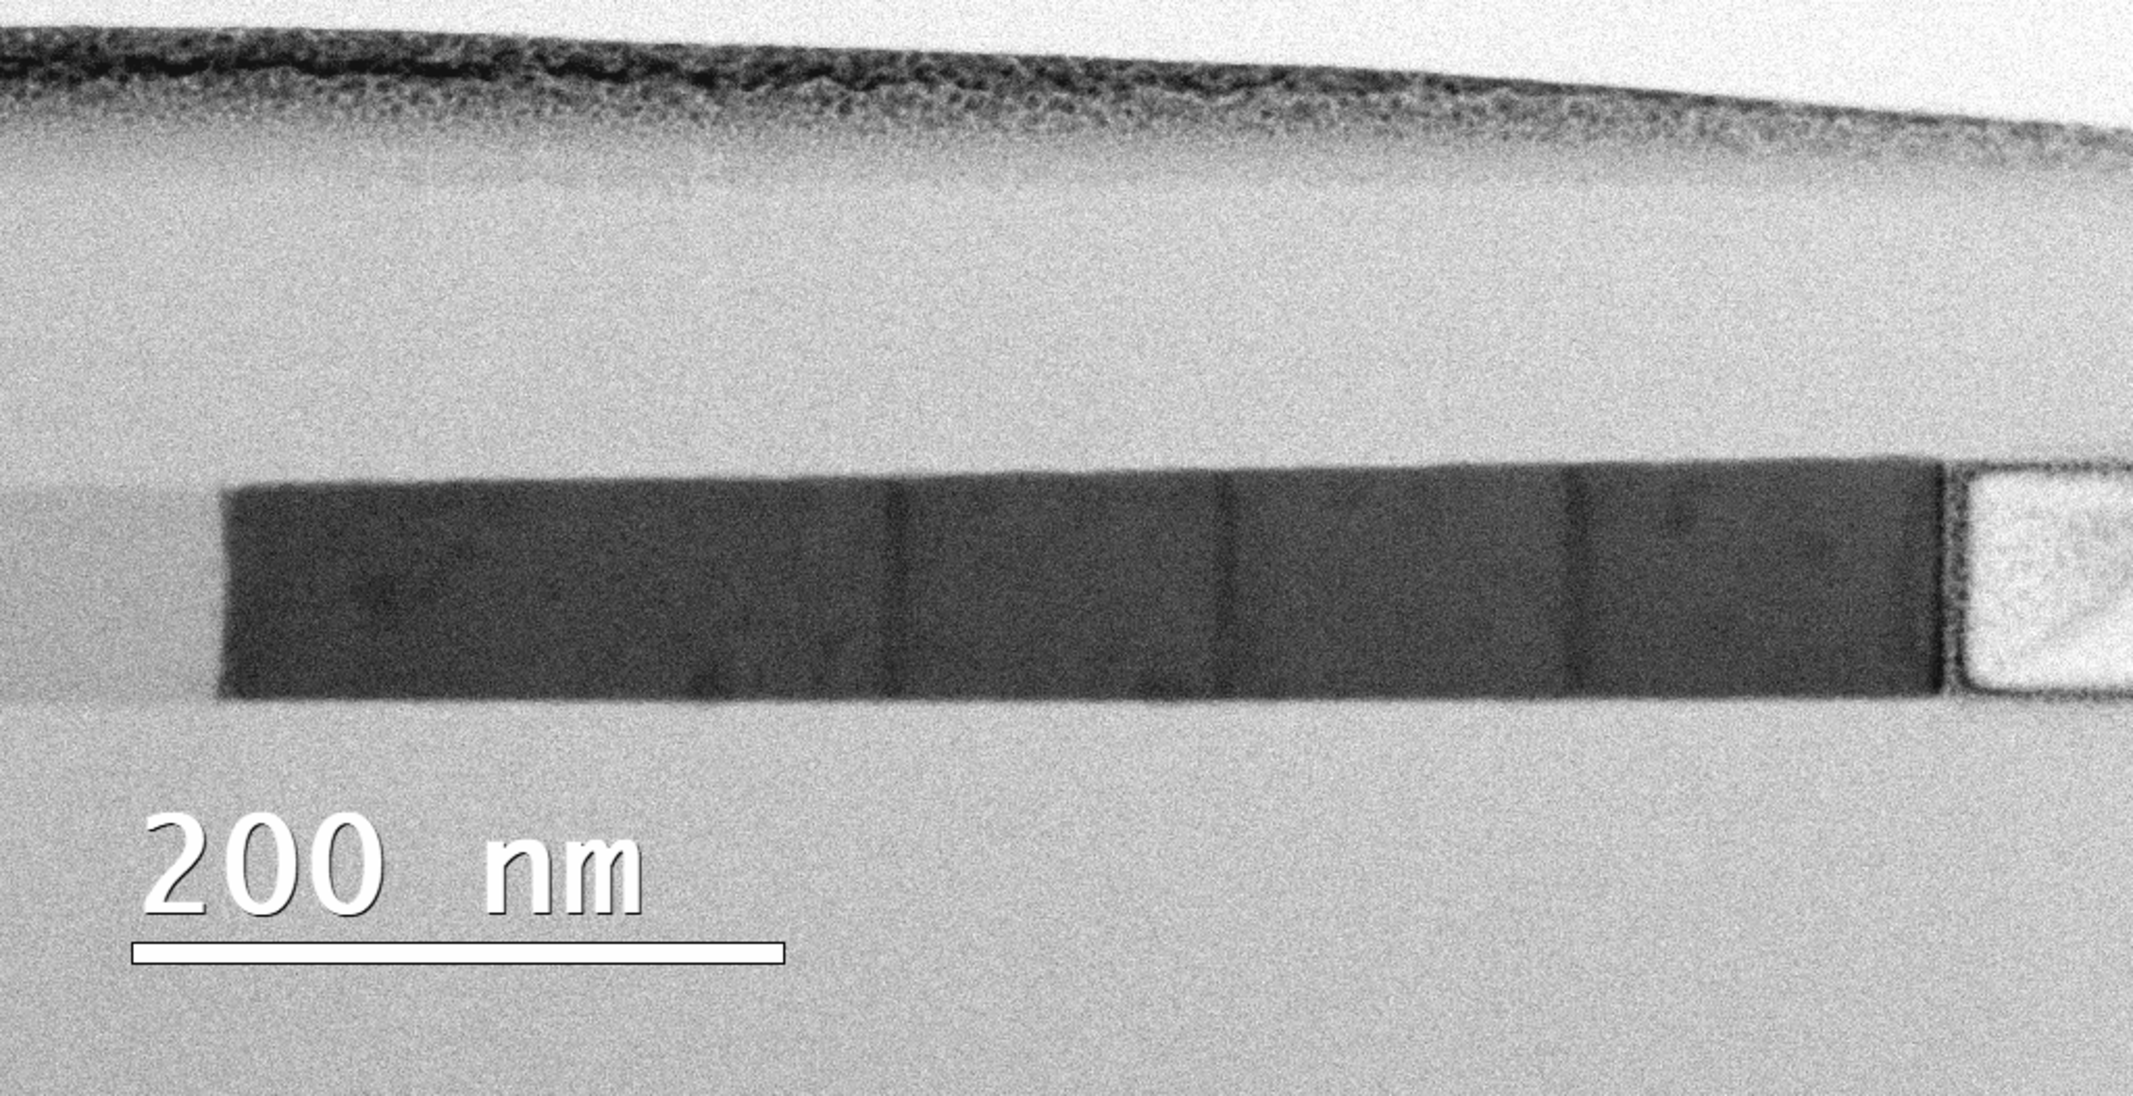
\includegraphics[width = 0.48\textwidth]{4_Properties/Fig/s5_OV.pdf}
    }
    \caption{\acs{mocvd} recipe and growth results for sample 5. \subref{subfig:recipe5} shows the \acs{mocvd} growth recipe. \subref{subfig:SEM_array} shows an \acs{sem_m} image of an array of nanowires. The image was recorded with the stage tilted \qty{52}{\degree}. An in-plane \hkl<1 1 0> direction runs parallel to the bottom margin of the image. \subref{subfig:s5_OV} sho3ws a \acs{bf}-\acs{stem_m} overview images of a nanowires. The \acs{si} seed is on the left of the III-V nanowire.}
    \label{fig:s5_recipe_microscopy}
\end{sidewaysfigure}

After examining the photoluminescence results of sample 4 (Figure~\ref{fig:s4_pl}) the recipe was adjusted to minimise the effect of the \acs{ingaas} nucleation layer. Previous experience in the research group at \acs{ibm} Research Europe - Zurich has shown that this layer, grown with a target composition of \ce{In0_.53Ga0_.47As}, has a positive effect on the nucleation yield of III-Vs on \acs{si}. However, once nucleation is achieved, it does not serve a further purpose in the experiments described in this chapter. 

Given its possible negative impact on the photoluminescence analysis of the samples, a new \acf{mocvd} recipe was created, shown in Figure~\ref{subfig:recipe5}. The step time for the nucleation \acs{ingaas} layer was reduced to \qty{30}{\second}. The deposition time of the \acs{inp} stabilisation layer was increased to \qty{450}{\second} to keep the \acs{ingaas} \acl{qw}s far from the nucleation layer. This was also meant to ensure the stabilisation of the single-facet \hkl{1 1 1} growth front, to avoid situations such as the one seen in the \qty{30}{\degree} cross-section of sample 4 (Figure~\ref{subfig:s4_OV}), where the first \acl{qw} followed a multi-faceted growth front. 

Part of one of the nanowire arrays designed in Figure~\ref{subfig:110_design2} was imaged at a \qty{52}{\degree} angle with \acs{sem_m}. The resulting image is shown in Figure~\ref{subfig:SEM_array}. The various elements of the \acs{tase} structures are visible. Various \acs{si} seeds are anchored to each rectangular \acs{si} backbone. The III-V semiconductor nanowires appear as the brighter segments after the seeds. The empty templates follow the III-V material, ending in the opening of the template visible in the centre of the image created by the \acf{icp} etching. 

Already in Figure~\ref{subfig:SEM_array}, the low competitiveness of the growth process is qualitatively inferable, as the length of the nanowires in the middle of the array is not noticeably different from that of the nanowires at the edges.

Figure~\ref{subfig:s5_OV} shows a \acs{bf}-\acs{stem_m} image of a nanowire from sample 5. The \acs{si} seed is on the left of the image. The variable thickness of the lamella, manifested by the decreasing height (from left to right) of the top platinum layer, leftover from \acs{fib} sample preparation, contributes to a progressive darkening of the \acs{inp} stabilisation layer towards the seed. Furthermore, the absence of a hold step after the nucleation layer makes the heterointerface between the arsenide and phosphide layer more "blurred". These factors make the now thin \acs{ingaas} layer not immediately identifiable by channelling contrast, unlike in Figure~\ref{subfig:s4_OV}.

All visible heterointerfaces, including the final facet of the nanowire exposed to the protective platinum on the right of the image, appear sharp in this image. The heterointerfaces also give the reader a snapshot of the growth front, which is composed of a single \hkl{1 1 1} facet after the \acs{inp} stabilisation layer.

\begin{table}
    \centering
    \caption{Growth rates for the superlattice region of sample 5.}
    \begin{tabular}{c|c c c|c c c}
       & \multicolumn{3}{c}{\acs{ingaas}} & \multicolumn{3}{|c}{\acs{inp}} \\
       material layer & well 1 & well 2 & well 3 & barrier 1 & barrier 2 & barrier 3 \\ \hline
       growth rates (\nmmin) & \num[separate-uncertainty=true]{43 (3)} & \num[separate-uncertainty=true]{39 (2)} & \num[separate-uncertainty=true]{44 (4)} & \num[separate-uncertainty=true]{28.0 (0.2)} & \num[separate-uncertainty=true]{30.2 (0.1)} & \num[separate-uncertainty=true]{32.7 (0.2)} \\ \hline \hline
    \end{tabular}
    \label{tab:s5_growth_rates}
\end{table}

\paragraph{Growth rate} The growth rate calculation methodology remains unchanged for this sample and consists of taking the average of \num{7} repeated measurements of layer thickness perpendicularly to each subsequent heterointerface. The error expresses the \qty{95}{\%} confidence interval around the growth rate value and it is assumed that the deposition time is error-free.

Table~\ref{tab:s5_growth_rates} summarises the growth rates for each material layer in the \acs{ingaas}-\acs{inp} \acl{qw} structure. The \acs{ingaas} growth rates remain similar to those calculated for sample 4, despite the halving of the \acs{ingaas} deposition time. On the contrary, \acs{inp} growth rate is higher by between \qty{7}{\nmmin} and \qty{10}{\nmmin}, despite the fact that the \acs{inp} deposition step time was not altered from the recipe used for sample 4 (Figure~\ref{subfig:recipe4}). 

This discrepancy in growth rate evolution for the \acs{inp} and \acs{ingaas} layers could indicate a small dependency of the growth rate on deposition time. This may be due to the time required to exchange the precursor molar fractions in the template becoming less and less negligible as the step time lowers.
\par

\begin{figure}
    \centering
    \subcaptionbox{
    \acs{eds} linescan: III atomic percentage vs position.
    \label{subfig:s5_III_0deg_linesc}
    }{
    \tikzsetnextfilename{s5_III_0deg_linesc}
    \begin{tikzpicture}
        \begin{axis}[
            width = 0.8\textwidth,
            height = 5cm,
            xlabel = Position (nm),
            ylabel = Composition (atomic \%),
            table/col sep=comma,
            %title = III element composition,
            legend pos=outer north east,
            ymin=0, ymax=100,
            xmin = 0, xmax=348.61
        ]
    \addplot [cb1_orange,] table[x=nm,y=Ga] {4_Properties/csv/s5_III_0deg_linesc.csv};
    \addplot [cb1_dark_blue,] table[x=nm,y=In] {4_Properties/csv/s5_III_0deg_linesc.csv};
    \addlegendentry{Ga}
    \addlegendentry{In}
    \end{axis}

    \end{tikzpicture}
    }
    \subcaptionbox{
    \acs{eds} linescan: V atomic percentage vs position.
    \label{subfig:s5_V_0deg_linesc}
    }{
    \tikzsetnextfilename{s5_V_0deg_linesc}
    \begin{tikzpicture}
        \begin{axis}[
            width = 0.8\textwidth,
            height = 5cm,
            xlabel = Position (nm),
            ylabel = Composition (atomic \%),
            table/col sep=comma,
            %title = V element composition,
            legend pos=outer north east,
            ymin=0, ymax=100,
            xmin = 0, xmax=348.61
        ]
    \addplot [cb1_orange,] table[x=nm,y=As] {4_Properties/csv/s5_V_0deg_linesc.csv};
    \addplot [cb1_dark_blue,] table[x=nm,y=P] {4_Properties/csv/s5_V_0deg_linesc.csv};
    \addlegendentry{As}
    \addlegendentry{P}
    \end{axis}

    \end{tikzpicture}
    }
    \caption{\acs{eds} linescan compositional data (in percentage) for the \subref{subfig:s5_III_0deg_linesc} III elements and \subref{subfig:s5_V_0deg_linesc} V elements across all three \acl{qw} of the sample seen in Figure~\ref{subfig:s5_OV}. The origin of the x-axis is situated before the first well and is the closest point to the \acs{si} seed. Higher position numbers (in nm) represent the scan moving along the \hkl{1 1 1} vector perpendicular to the growth front away from the seed.}
    \label{fig:s5_0deg_linescans}
\end{figure}

\paragraph{\acs{eds} analysis} An \acs{eds} linescan measurement was carried out across the \acs{inp}-\acs{ingaas} \acl{qw} region. After elaboration with the \acf{gms}, the two composition profiles, one for III elements, and the other for V elements, is reported in Figure~\ref{fig:s5_0deg_linescans}. The linescan was recorded starting from before the first \acl{qw} and moved across the superlattice towards the end of the wire, stopping after the third \acl{qw}.

Figure~\ref{subfig:s5_III_0deg_linesc} shows a graph of the concentration, in atomic percentage, of \acl{ga} and \acl{in}, calculated from the relative intensity of their respective L\(_\alpha\) lines and their \acs{eds} cross-section. Unlike previous samples, the \acl{ga} contamination following the \acs{ingaas} \acl{qw} is absent in the starting portion of the \acs{inp} well. The lower overall concentration of \acl{ga} in the \acl{qw} could, however, simply make a trailing \acl{ga} contamination too small to be noticeable above the \qty{10}{\%} noise level that affects the concentration measurement. The composition of the \acl{qw} can be estimated at approximately \ce{In0_.4Ga0_.6As}.

The atomic percentage concentrations of \acl{as} and \acl{p} in Figure~\ref{subfig:s5_V_0deg_linesc} were calculated from their respective K\(_\alpha\) lines. The noise level is around \qty{20}{\%}. The presence of a post-\acs{ingaas} \acl{as} contamination in the \acs{inp} barrier layer remains distinguishable from background noise. This is particularly evident when looking at the steepness of the arsenic peaks at each arsenide-phosphide interface. The leading interface is almost vertical while the trailing interface curves down more gently.

These repeated observations (Figures~\ref{fig:s3_linescans}, \ref{fig:s4_0deg_linescans}, and \ref{fig:s5_0deg_linescans}) point to an \acs{ingaas} to \acs{inp} heterointerface definition limitation inherent to the stacking of the material layers. Although the changes in the hold step following the \acs{ingaas} layer did not contribute to the interface definition, they did solve the III-element integration delay issue, as the \acl{as} and \acs{ga} profile remain reliably synced in multiple growth runs.
\par

\begin{figure}
    \centering
    \tikzsetnextfilename{s5_pl}
    \begin{tikzpicture}
        \begin{axis}[
            width = 0.8\textwidth,
            height = 5cm,
            xlabel = Wavelegth (nm),
            ylabel = Intensity (a.u.),
            table/col sep=comma,
            %title = Photoluminescence Spectrum,
            legend pos=outer north east,
            ymin=0, ymax=1000,
            xmin = 1268.8, xmax=1600.3
            ]
            \addplot [cb1_dark_blue,] table[x=wavelength,y=intensity] {4_Properties/csv/s4_pl.csv};
            \addplot [cb1_orange,] table[x=wavelength,y=intensity] {4_Properties/csv/s5_pl.csv};
            \addlegendentry{Sample 4}
            \addlegendentry{Sample 5}
        \end{axis}
    \end{tikzpicture}
    \caption{Photoluminescence spectra of two nanowires from samples 4 and 5. These spectra were kindly recorded by Markus Scherrer.}
    \label{fig:s5_pl}
\end{figure}

\paragraph{Photoluminescence analysis} Figure~\ref{fig:s5_pl} compares a photoluminescence spectrum recorded for sample 5 with that recorded for sample 4 and shown in Figure~\ref{fig:s4_pl}. The measurement conditions were left largely unchanged. The main alterations affected the sample temperature, which was \qty{-100}{\kelvin} instead of \qty{-200}{\kelvin}, and the excitation wavelength, set at \qty{1060}{\nano\metre} instead of \qty{1060}{\nano\metre}. Therefore, despite the small change in wavelength, the material targeted for analysis remained \acs{ingaas}.

The emission peak of the \acl{qw}s is found at a wavelength lower than that of the peak of sample 4. This could be due to the higher \acl{in} concentration seen in Figure~\ref{subfig:s5_III_0deg_linesc}, however, as the peak is much narrower for this sample, a \acl{qw} effect could be present. Unfortunately, due to the noise level of the \acs{eds} composition profiles, it is difficult to attribute the spectral changes to either of these changes.
\par

\subsection{Merge Structures}

\begin{figure}
    \centering
    \subcaptionbox{
        \acs{sem_m} image of merge structures before lamella cut-off.
        \label{subfig:SEM_merge_bulk}
    }{
        \tikzsetnextfilename{SEM_merge_bulk}
        \begin{tikzpicture}
            \node[inner sep=0pt] (image) at (0,0) {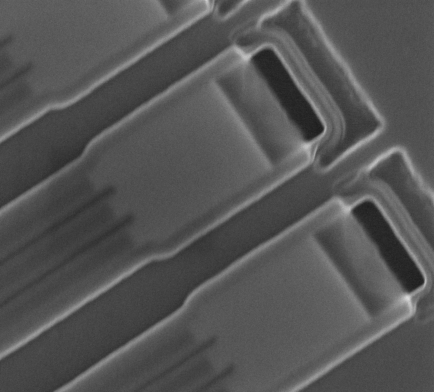
\includegraphics[width = 0.34\textwidth]{4_Properties/Fig/SEM_merge_bulk.pdf}};
            \draw[|-|, white] (0.3,-2) -- (2,-2)  node[midway, anchor=south, white] {\qty{500}{\nano\metre}};
        \end{tikzpicture}
    }
    \subcaptionbox{
        \acs{sem_m} image of a lamella containing merge structures during \acs{fib} thinning.
        \label{subfig:SEM_merge_lamella}
    }{
        \tikzsetnextfilename{SEM_merge_lamella}
        \begin{tikzpicture}
            \node[inner sep=0pt] (image) at (0,0) {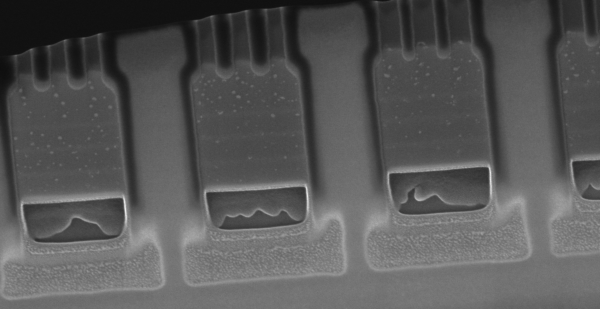
\includegraphics[width = 0.60\textwidth]{4_Properties/Fig/SEM_merge_lamella.pdf}};
            \draw[|-|, white] (1.5,-2) -- (3.7,-2)  node[midway, anchor=south, white] {\qty{500}{\nano\metre}};
        \end{tikzpicture}
    }
    \caption{\acs{sem_m} image of merge structures taken \subref{subfig:SEM_merge_bulk} before and \subref{subfig:SEM_merge_lamella} during \acs{fib} lamella cut-out and thinning.}
    \label{fig:SEM_merge}
\end{figure}

In addition to the nanowire arrays (Figure~\ref{subfig:SEM_array}), sample 5 contained the multi-seed structures shown in Figure~\ref{fig:SEM_merge}. These structures were processed (template opening, sacrificial \acl{si} etch-back, and \acs{mocvd} growth) at the same time as the arrays seen in the previous section. In these multi-seed structures, three seed regions are provided for III-V nucleation. The template design then forces the three growing crystals into a larger template area where they can come into contact with each other and merge. This type of structure is expected to introduce defects at the merging locations, even in the case of simultaneous nucleation on all three seeds \cite{Mauthe2021}.

Various avenues of stress relaxation in epitaxially grown III-V crystals induce alterations in their lattice, making the merging of two different crystals a prime defect-nucleating event \cite{Jacobsson2015}. The nucleation of defects is common even in situations where lattice rotations follow the symmetry rules of the crystals \cite{Rossi2023}. If small (\qty{1}{\degree} to \qty{5}{\degree}) tilt of the III-V crystalline axis from the \hkl<1 1 1> axis occurs to relax stress, as seen in sample 4 (Figure~\ref{subfig:s4_OV}) it is expected to lead to a similar defect-nucleating situation. In contrast, under optimised growth conditions, the merging of two different crystals can result in defect-free material \cite{Imanishi2012}, leading to improvements in the crystalline quality of large-area III-V semiconductor films \cite{Imade2014}.

Figure~\ref{subfig:SEM_merge_bulk} shows the merge structures as they appear after \acs{mocvd} growth. In this top-down \acs{sem_m} image, the templates are orientated along an in-plane \hkl<1 1 1> direction and present a single \hkl{1 1 1} end facet. The III-V material can be seen filling the areas corresponding to the three seeds without any noticeable voids. 

The \acs{sem_m} image in Figure~\ref{subfig:SEM_merge_lamella} shows the same structures already seen in Figure~\ref{subfig:SEM_merge_bulk} in the final phases of \acs{fib} processing. The lamella was cut using the "plane view" technique (Figure~\ref{fig:110_FIB} left) to access multiple structures simultaneously on a \hkl<1 1 0> viewing axis at the \acs{stem_m}. Three lighter lines are already visible in each structure with \acs{sem_m} at this magnification level.

\begin{figure}
    \centering
    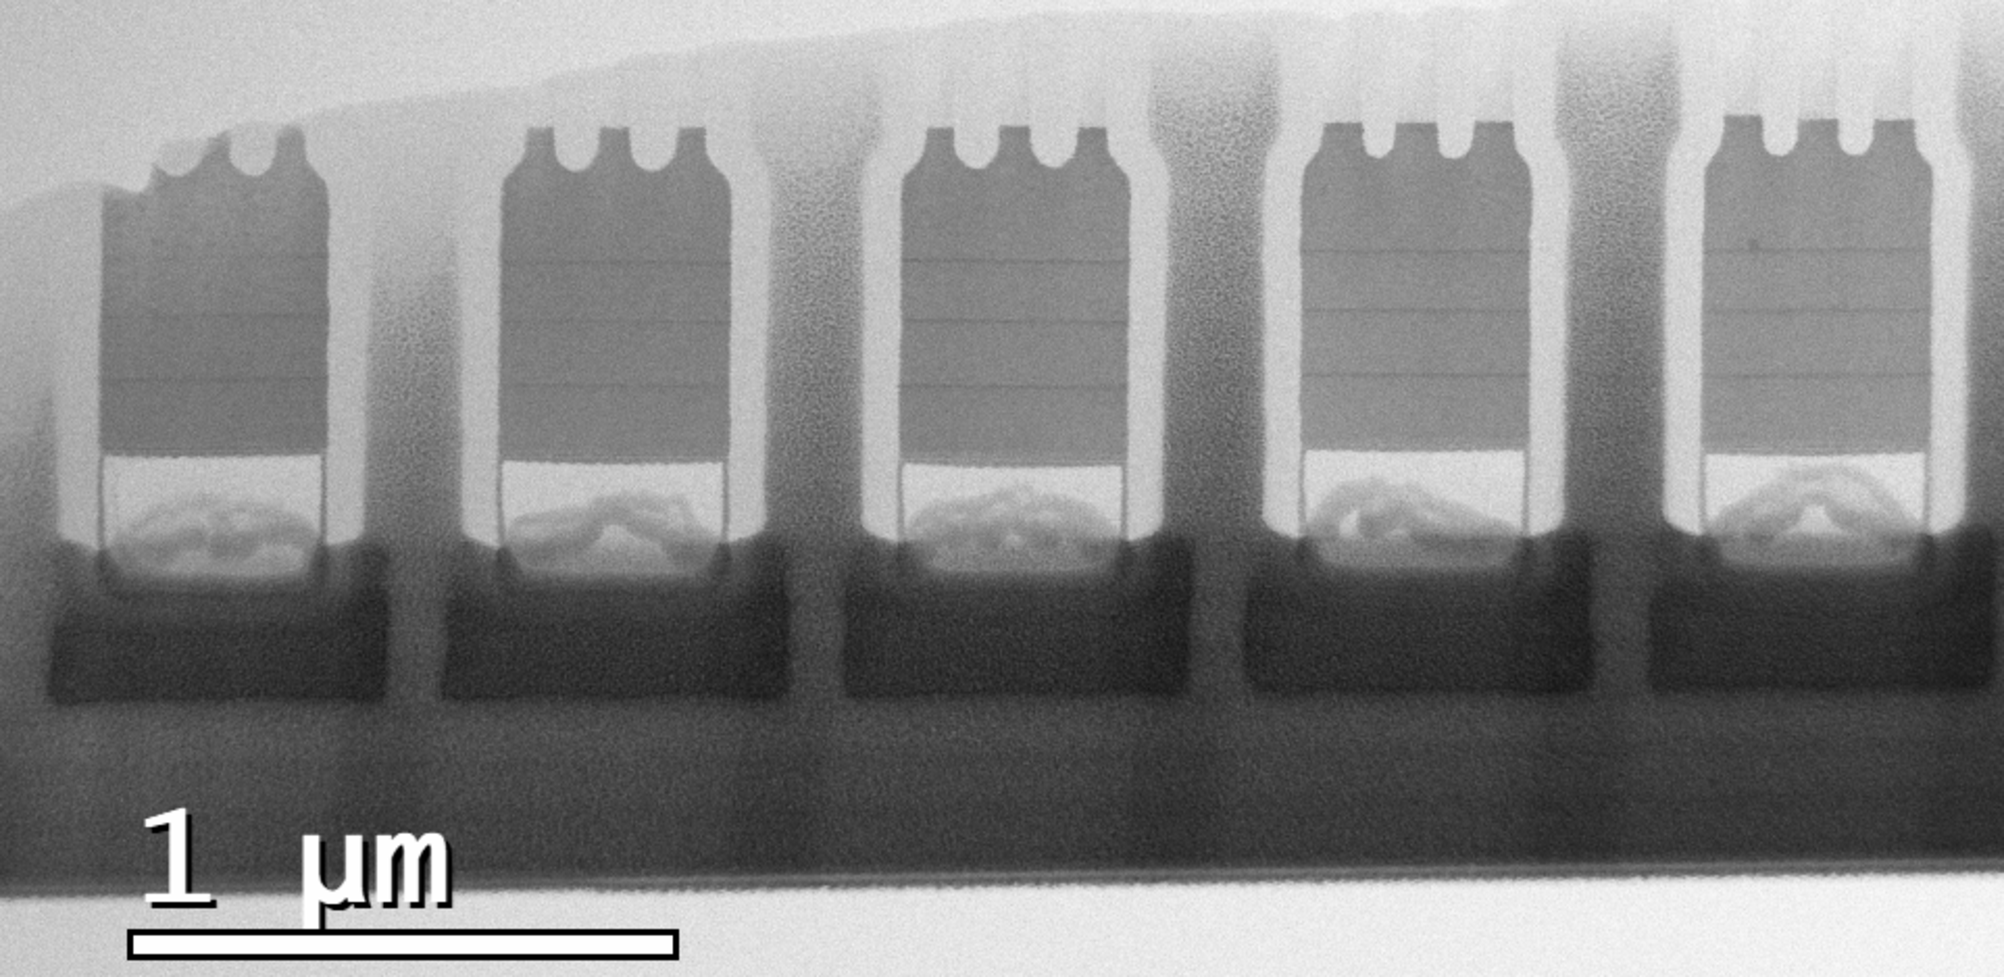
\includegraphics[width=\textwidth]{4_Properties/Fig/merge_OV.pdf}
    \caption{\acs{bf}-\acs{stem_m} overview image of the lamella containing five merge structures \cite{Brugnolotto2023_2}.}
    \label{fig:merge_ov}
\end{figure}

In Figure~\ref{fig:merge_ov}, each structure's three \acl{si} seeds appear at the top of the lamella. The (comparatively) electron transparent \acs{sio2} template outlines each of the five III-V structures. The \acs{fib} thinning partially damaged the leftmost structure, as too much material was removed from the seed area at the top left most of the lamella. The varying thickness of the lamella can be inferred by the darkness of the platinum layer between the III-V structure. Despite the best efforts made during \acs{fib} lamella preparation, the lamella is slightly thicker towards the bottom of the image, but this does not affect the quality of the image in the structure area, at this magnification level.

The first three structures have \qty{50}{\nano\metre} wide seed areas, while the two on the right have \qty{70}{\nano\metre} wide seeds. This small structural difference does not result in any appreciable change in the final III-V crystals, which all follow the template shape. The three lines corresponding to the arsenide layers are better visible in this \acs{bf}-\acs{stem_m} image, and all appear at the same distance from the \acs{si} seed.

\begin{figure}
    \centering
    \subcaptionbox{
        \acs{bf}-\acs{stem_m} overview image.
        \label{subfig:STEM_merge_structure_ov}
    }{
        \tikzsetnextfilename{SEM_merge_structure_ov}
        \begin{tikzpicture}
            \node[inner sep=0pt] (image) at (0,0) {\includegraphics[width = 0.48\textwidth]{4_Properties/Fig/merge_structure_OV.pdf}};
            \node[anchor=south, white] at (3.4,1.1) {\num{1}};
            \node[anchor=south, white] at (3.4,-0.5) {\num{2}};
            \node[anchor=south, white] at (3.4,-2.2) {\num{3}};
        \end{tikzpicture}
    }
    \subcaptionbox{
        \acs{df}-\acs{tem_m} overview image.
        \label{subfig:TEM_merge_structure_ov}
    }{
        \includegraphics[width=0.48\textwidth]{4_Properties/Fig/TEM_merge_structure_OV.pdf}
    }
    \subcaptionbox{
        Seed 1.
        \label{subfig:STEM_merge_seed1}
    }{
        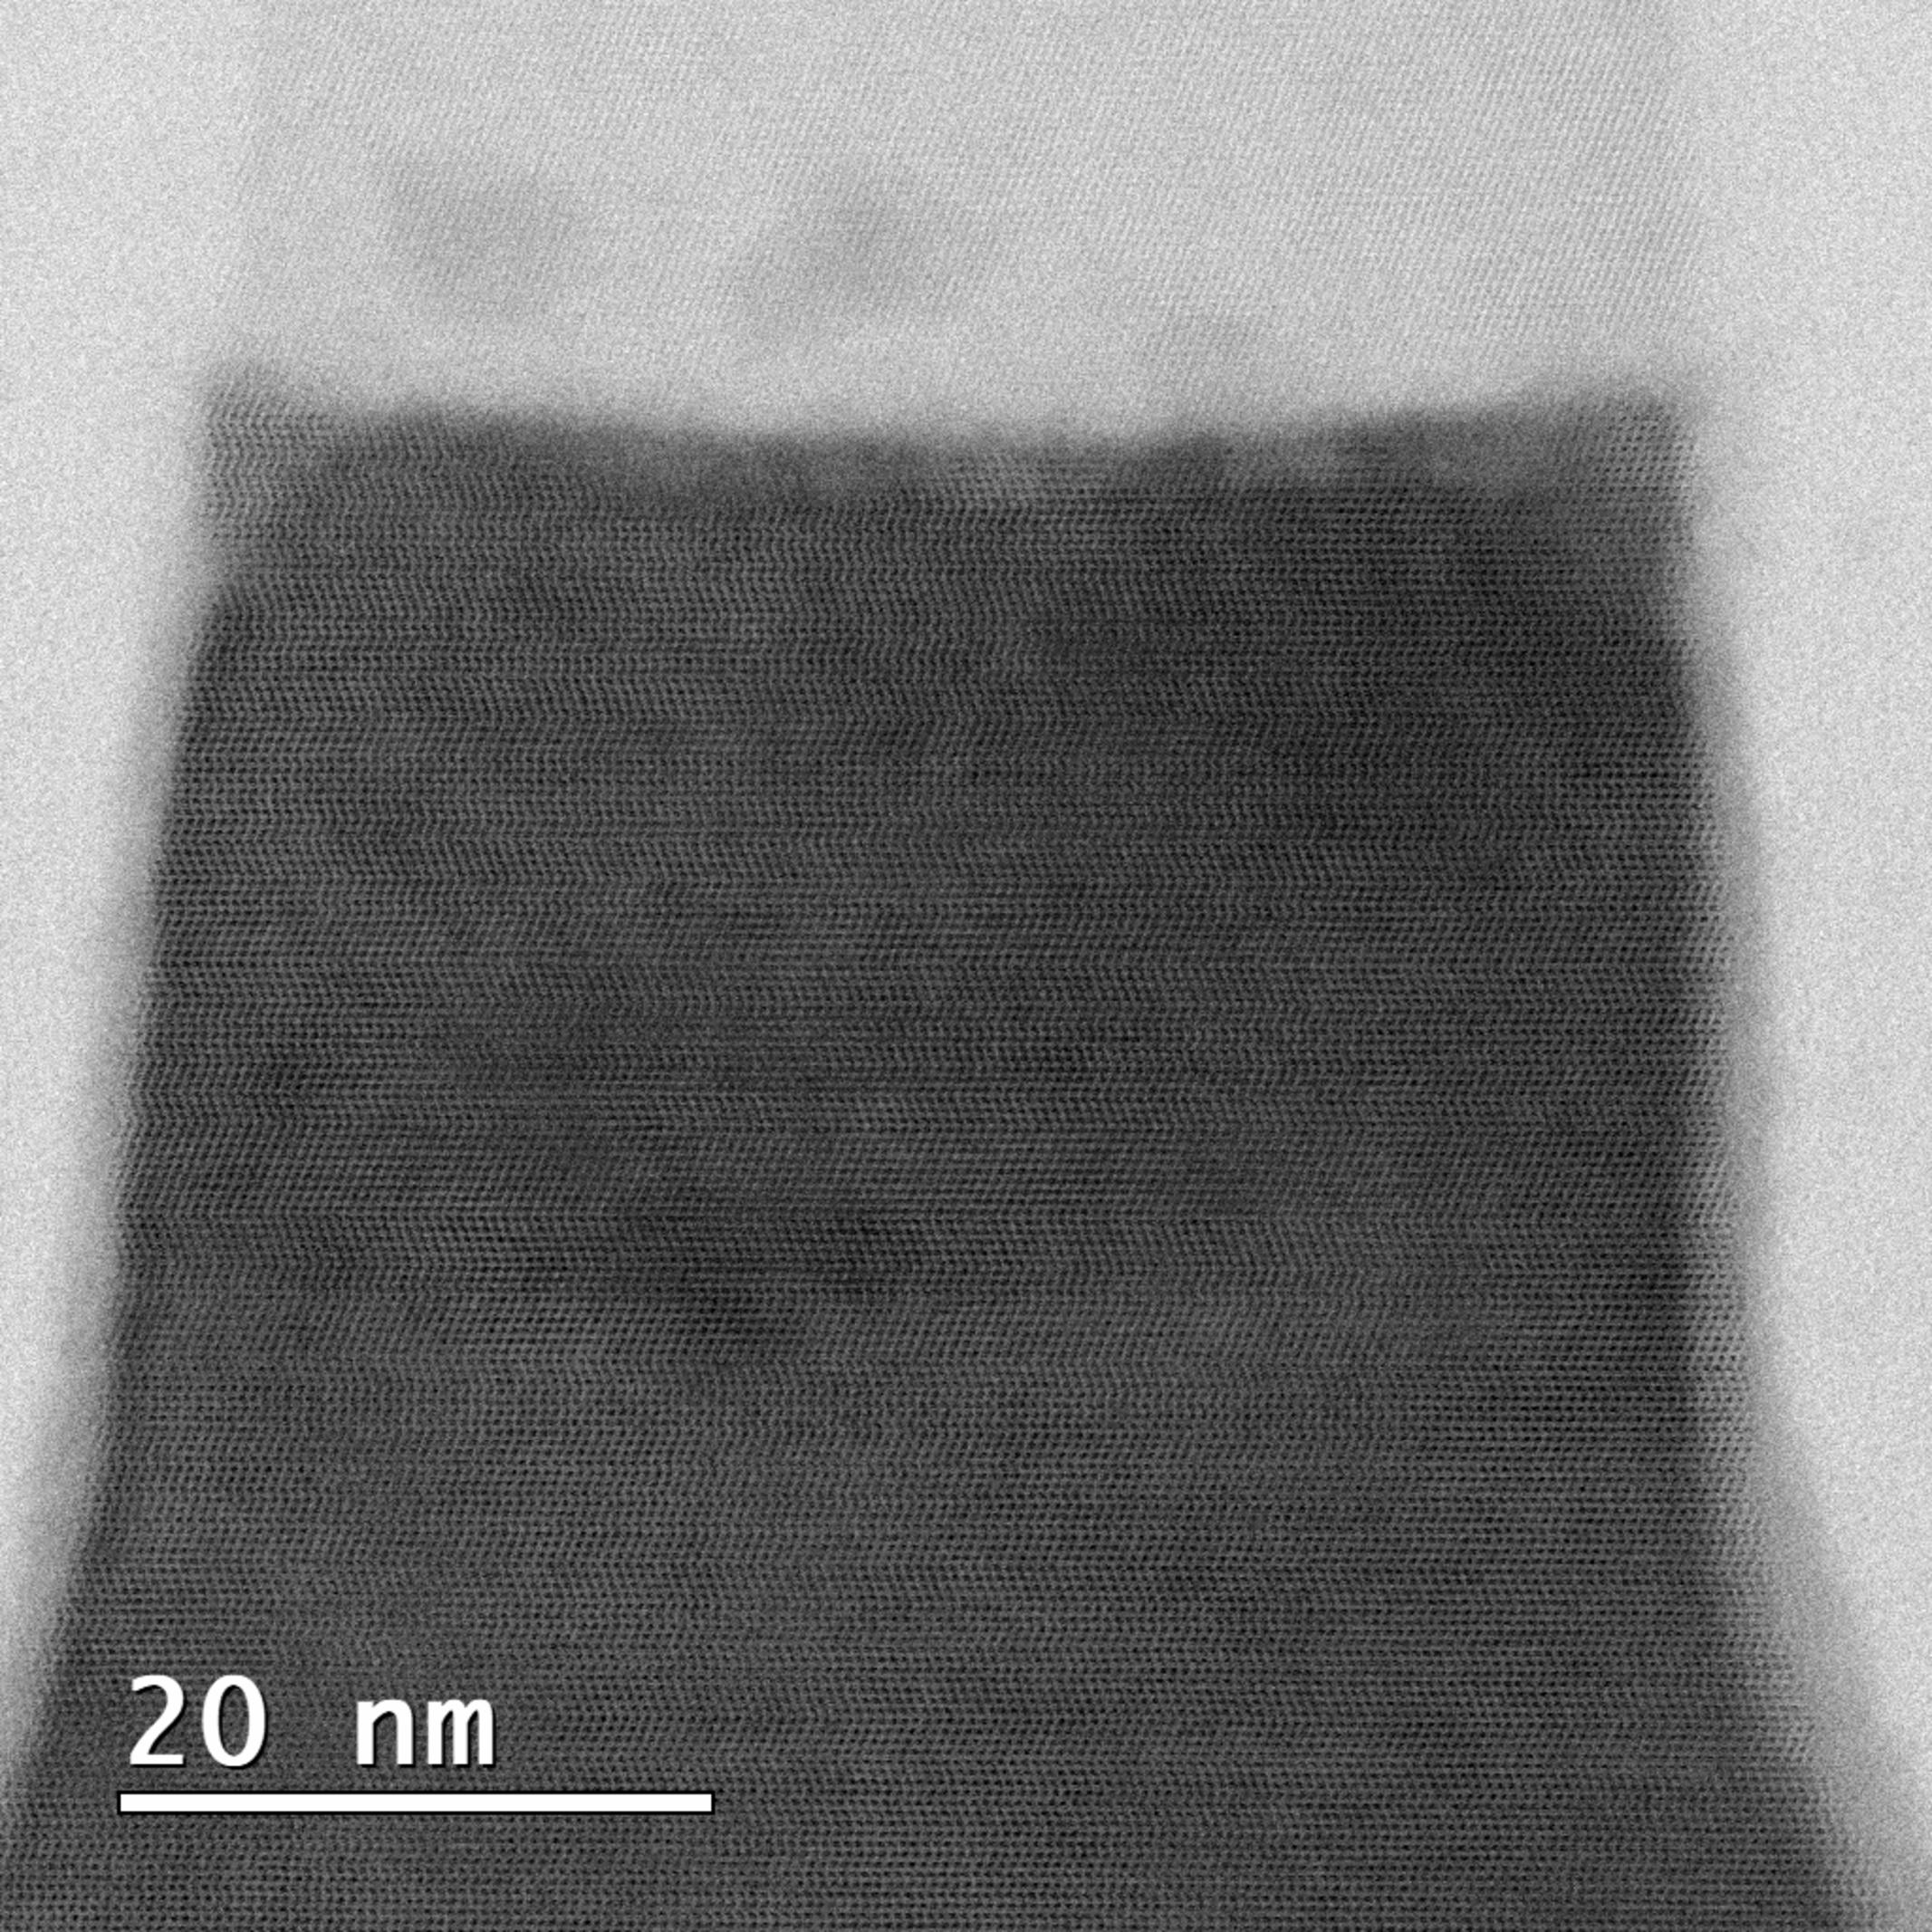
\includegraphics[width=0.24\textwidth]{4_Properties/Fig/STEM_merge_seed1.pdf}
    }
    \subcaptionbox{
        Seed 2.
        \label{subfig:STEM_merge_seed2}
    }{
        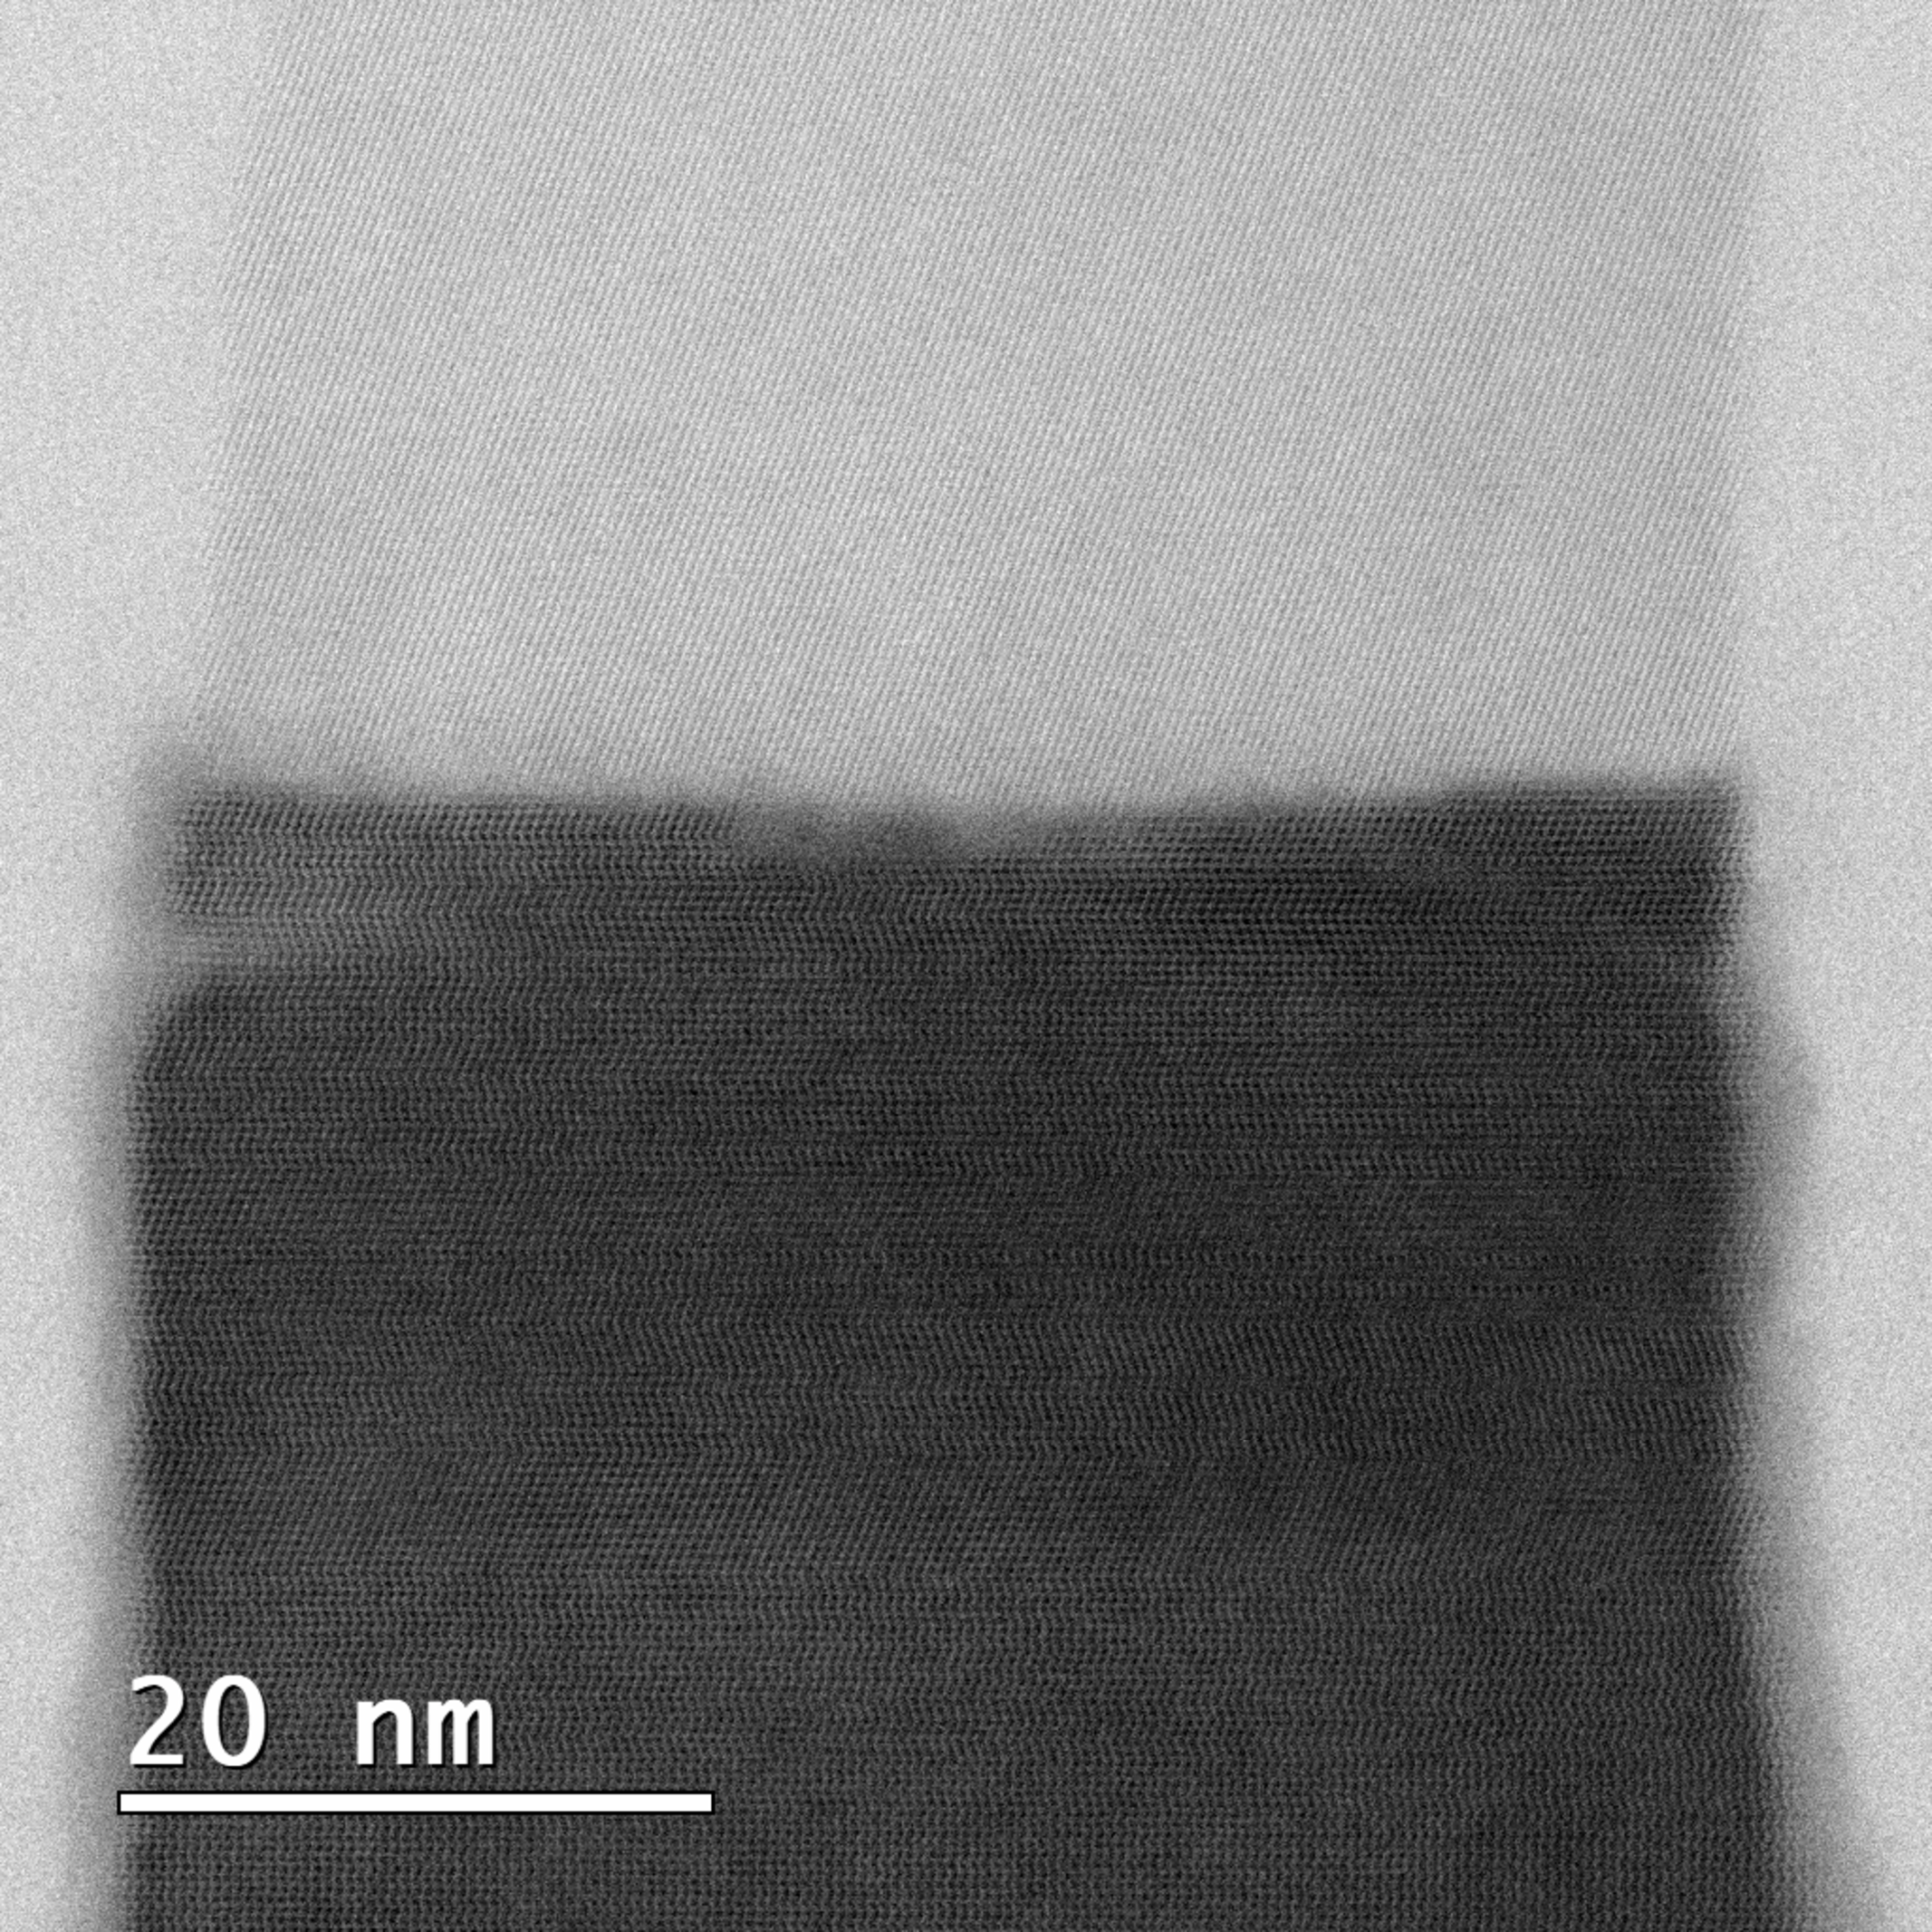
\includegraphics[width=0.24\textwidth]{4_Properties/Fig/STEM_merge_seed2.pdf}
    }
    \subcaptionbox{
        Seed 3.
        \label{subfig:STEM_merge_seed3}
    }{
        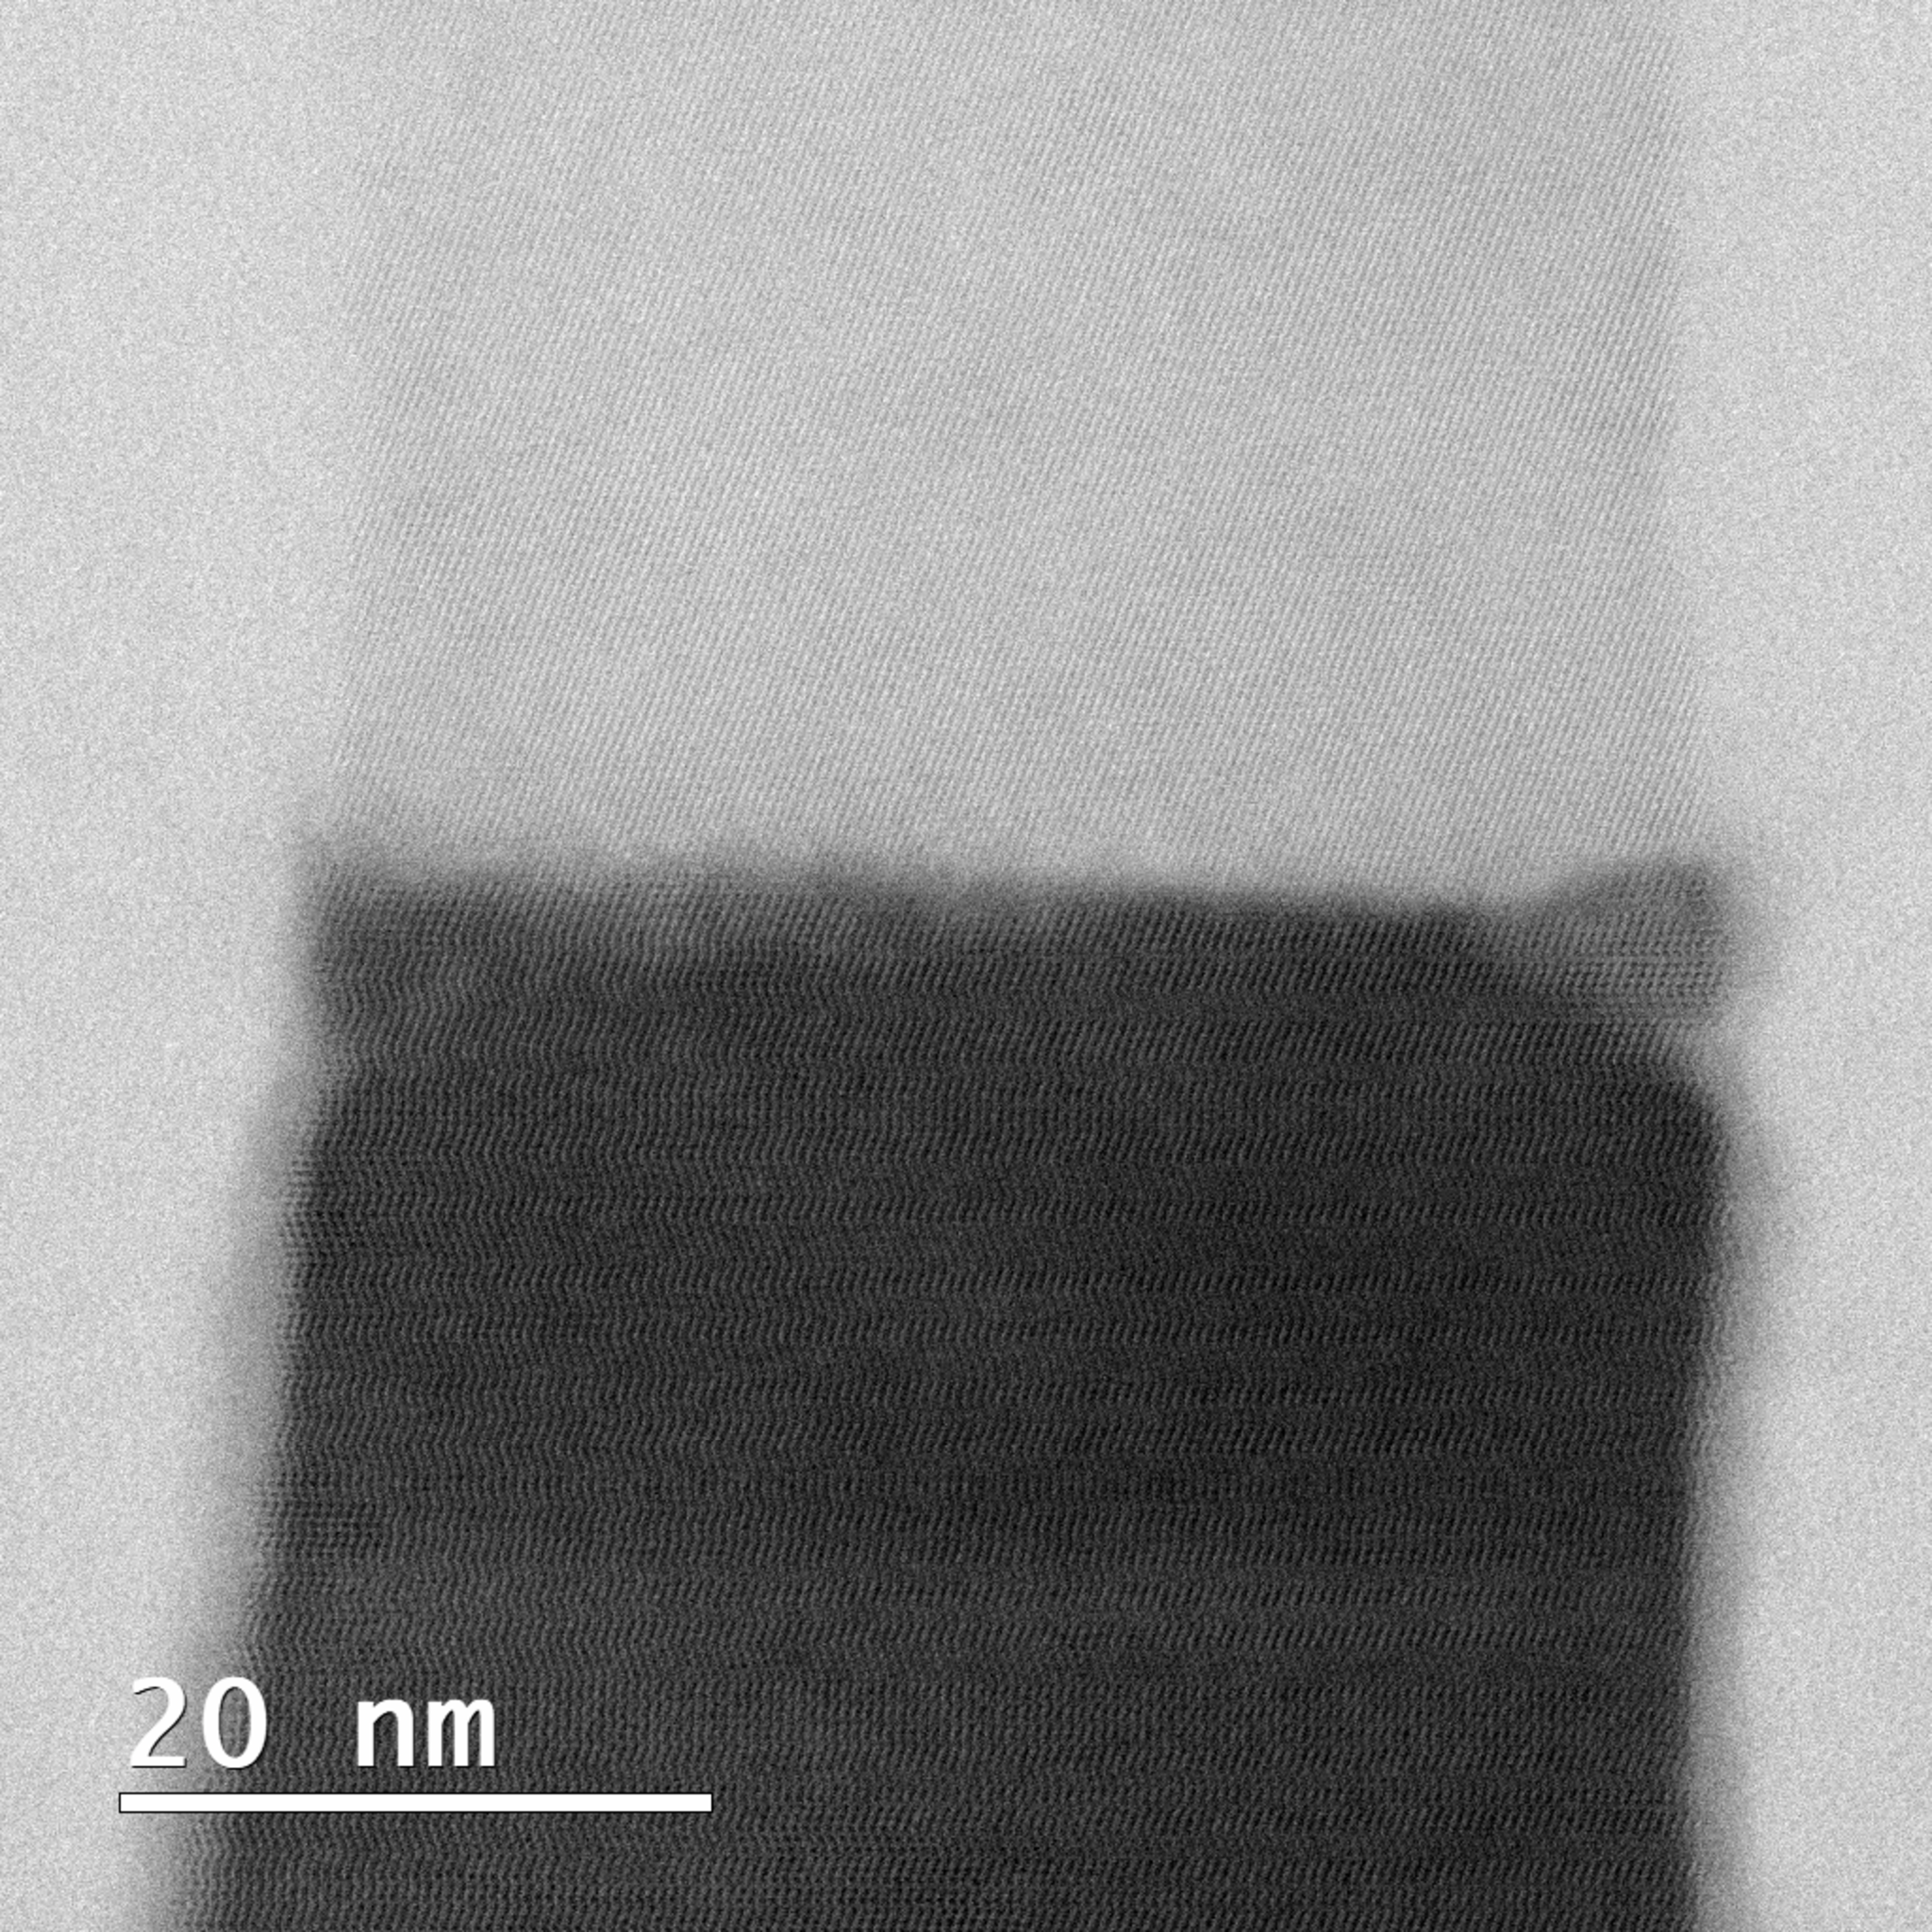
\includegraphics[width=0.24\textwidth]{4_Properties/Fig/STEM_merge_seed3.pdf}
    }
    \caption{\subref{subfig:STEM_merge_structure_ov} \acs{bf}-\acs{stem_m} and \subref{subfig:TEM_merge_structure_ov} \acs{df}-\acs{tem_m} overview images of a single merge structure. \subref{subfig:STEM_merge_seed1}, \subref{subfig:STEM_merge_seed2}, and \subref{subfig:STEM_merge_seed3} are \acs{bf}-\acs{stem_m} images of the nucleation areas 1, 2, and 3 as marked in \subref{subfig:STEM_merge_structure_ov}. \subref{subfig:TEM_merge_structure_ov} was kindly recorded by Michael Stiefel.}
    \label{fig:merge_ov_seeds}
\end{figure}

The nucleation areas of this structure are shown in high-resolution \acs{bf}-\acs{stem_m} images in Figures~\ref{subfig:STEM_merge_seed1}, \ref{subfig:STEM_merge_seed2}, and \ref{subfig:STEM_merge_seed3}. The \acl{si} seed is visible at the top of the images. The \acs{si} / III-V interface is well defined, showing the epitaxial relationship between the two lattices. The crystal appears to have nucleated towards the centre of the \acs{si} seed surface at all three nucleation sites. The \acs{ingaas} nucleation layer appears lighter in correspondence to the corners of the seed surface, likely due to a smaller amount of material in that area. As the crystal grows, it fills the \qty{50}{\nano\metre} wide template within the first 25 atomic bilayers.

The presence of an initial \acs{ingaas} followed by the \acs{inp} stabilisation layer within all three nucleation areas confirms that the simultaneous nucleation of three crystals has occurred for each structure. Once they have grown out of the \acs{sio2} separators, these three crystals must merge into one in the following template region. As seen in both Figures~\ref{subfig:STEM_merge_structure_ov} and \ref{subfig:TEM_merge_structure_ov}, the template is completely filled with III-V material, which has grown into the shape of the template. This excludes the formation of voids in this growth regime; however, the nucleation of point, line, and plane defects is still possible in the areas where the three crystals have come into contact with each other. 

It is important to note that this occurs even though the thickness of the \acs{ingaas} layer is different in the three seed regions. Seed one has a \acs{ingaas} thickness of \qty[separate-uncertainty=true]{28.3 (0.8)}{\nano\metre}, seed two shows a \qty[separate-uncertainty=true]{24.4 (0.3)}{\nano\metre} thick \acs{ingaas} nucleation layer, and the third nucleation layer has a length of \qty[separate-uncertainty=true]{23.1 (0.9)}{\nano\metre}. All three numbers are the result of averaging seven repeated measurements, and their errors represent the \qty{95}{\%} confidence interval. 

The presence of three heterolayers for each structure is reflected in the single-structure \acs{bf}-\acs{stem_m} and \acl{df} \acl{tem_m} (\acs{df}-\acs{tem_m}) overviews of Figures~\ref{subfig:STEM_merge_structure_ov} and \ref{subfig:TEM_merge_structure_ov}. The latter \acs{tem_m} image was recorded by Michael Stiefel, as was Figure~\ref{subfig:merge_region}. These three heterolayers are arsenide heterostructures, as shown by the contrast with the surrounding \acs{inp}, delimited by two single-facet \hkl{1 1 1} heterointerfaces. The similarity of these heterostructures to those seen in single nucleation nanowires, such as those in Figures~\ref{subfig:s5_OV} and \ref{subfig:s4_OV}, suggests that a highly ordered growth dynamic takes place in the template.

\begin{figure}
    \centering
    \subcaptionbox{
        \acs{bf}-\acs{tem_m} image of a likely merging region.
        \label{subfig:merge_region}
    }{
        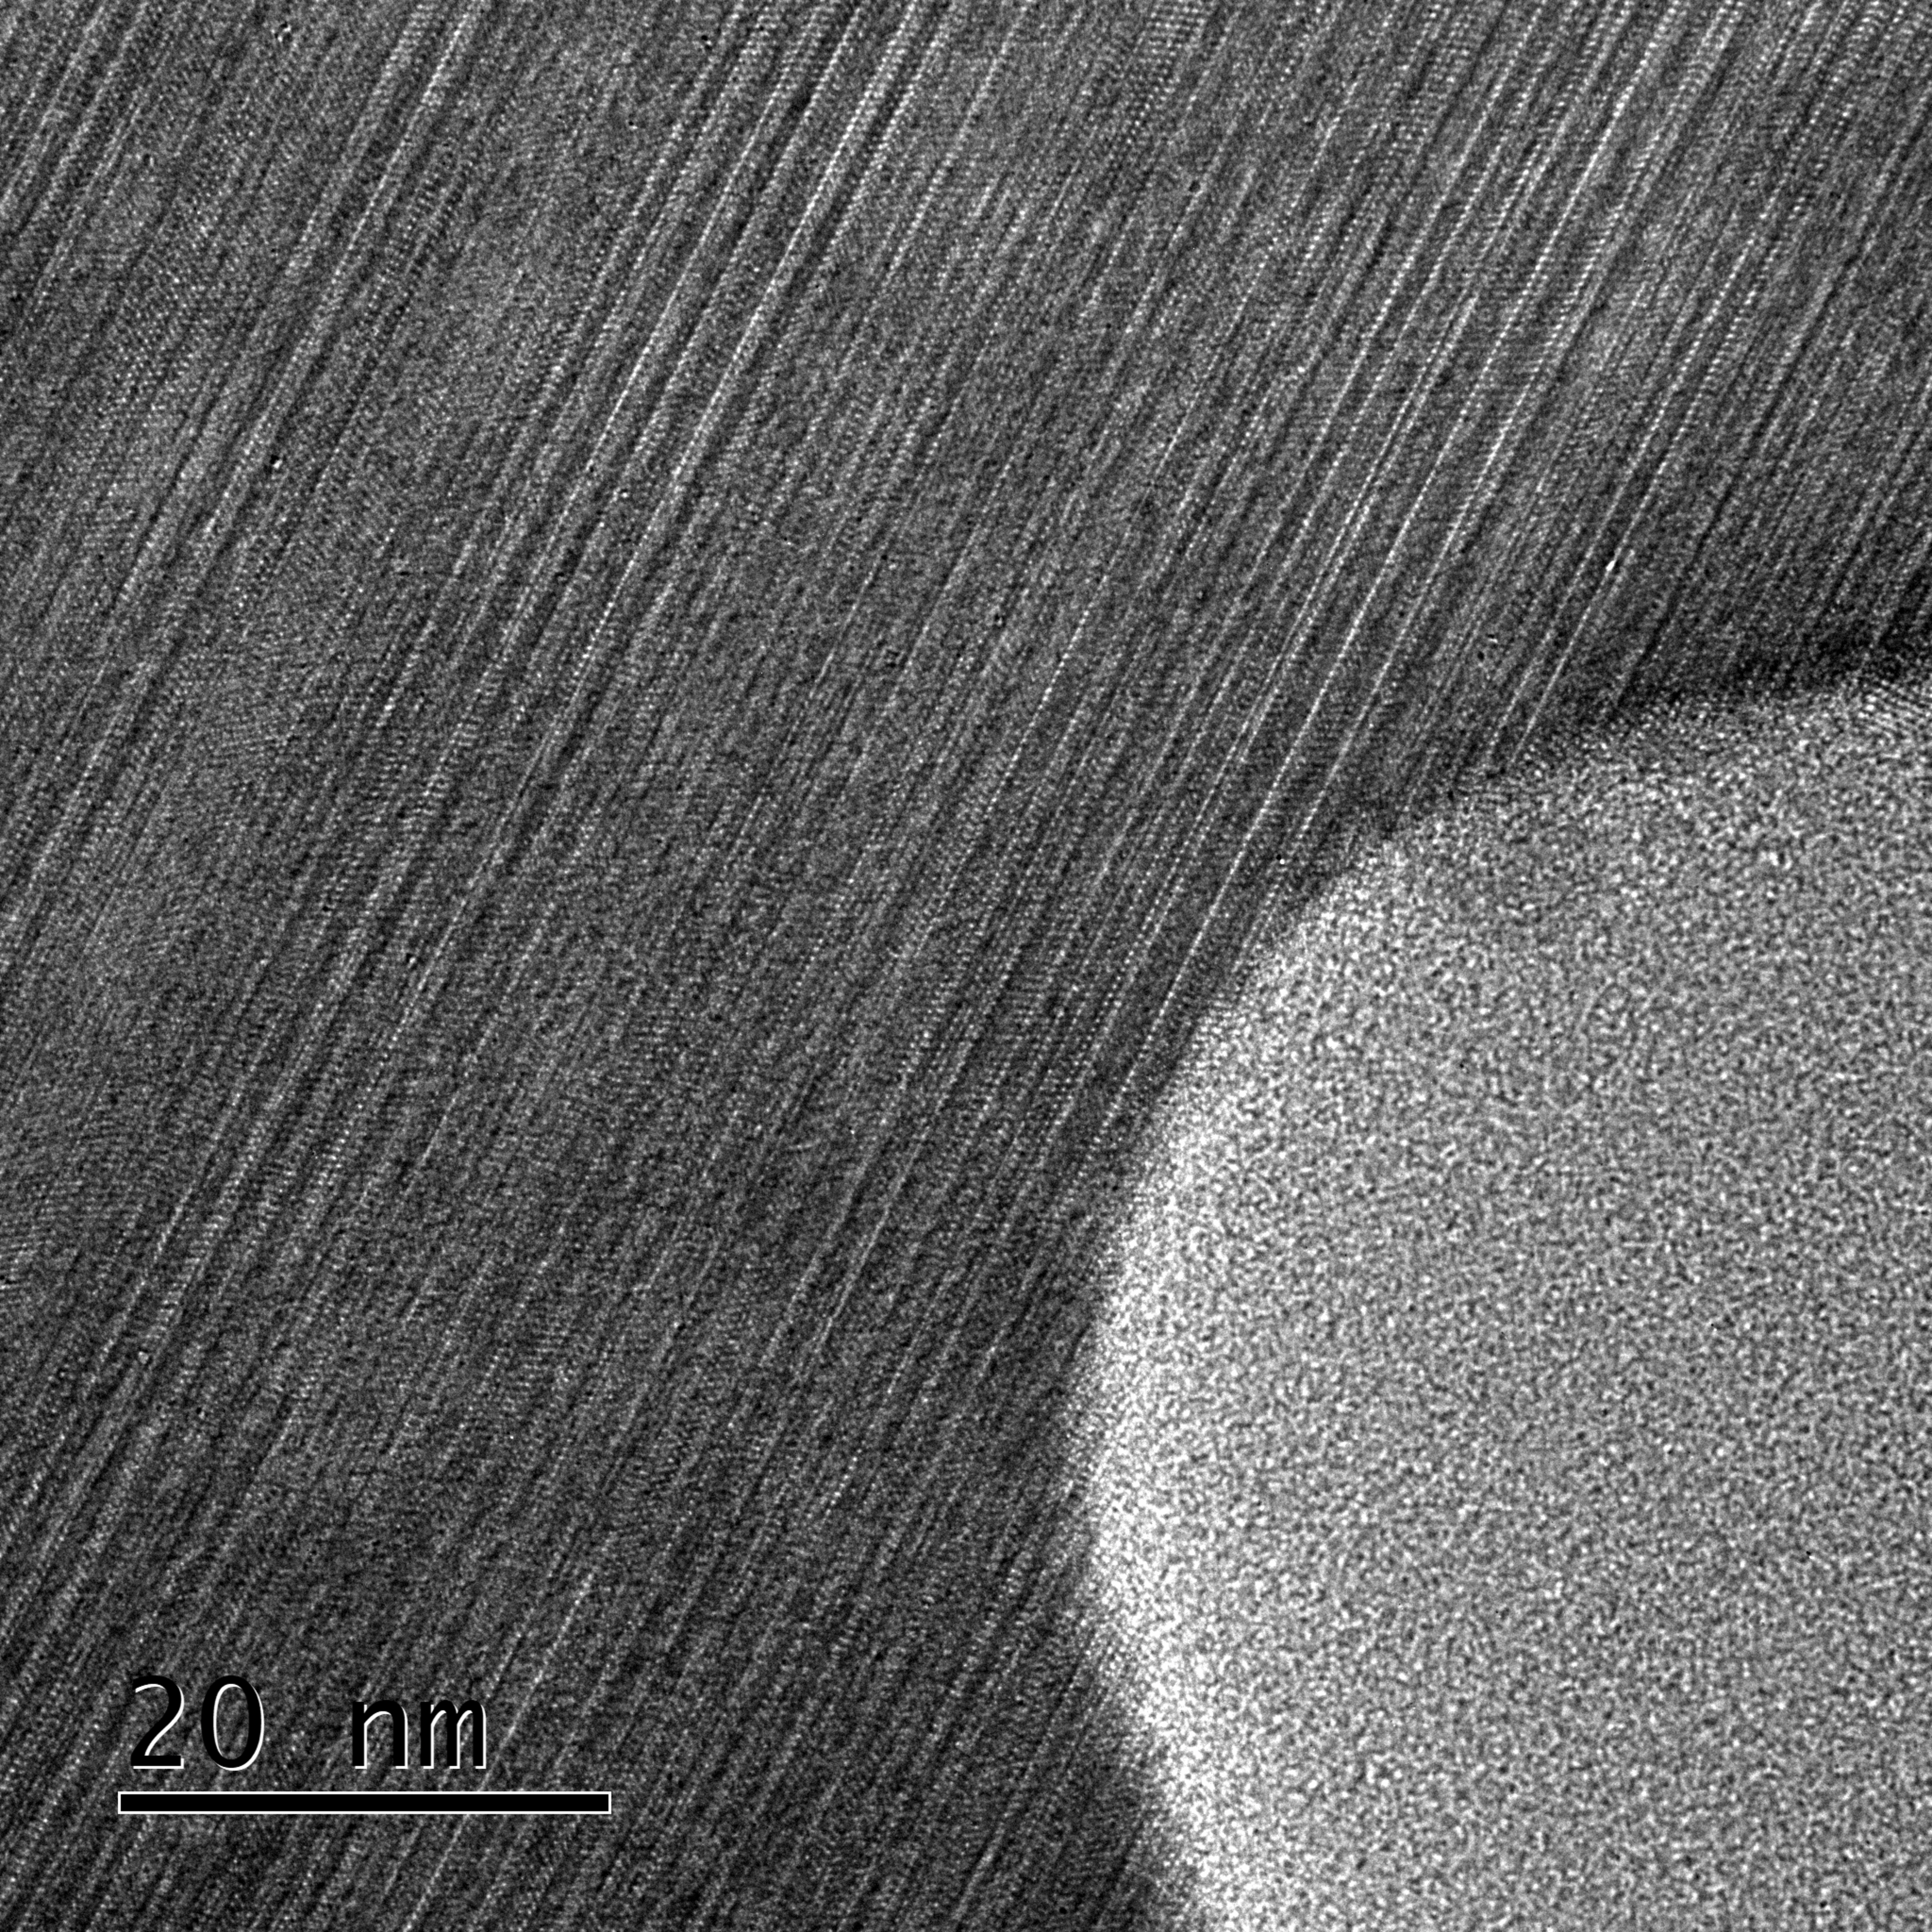
\includegraphics[width=0.48\textwidth]{4_Properties/Fig/merge_region.pdf}
    }
    \subcaptionbox{
        \acs{bf}-\acs{stem_m} image of a \acl{qw} \cite{Brugnolotto2023_2}.
        \label{subfig:merge_qw}
    }{
        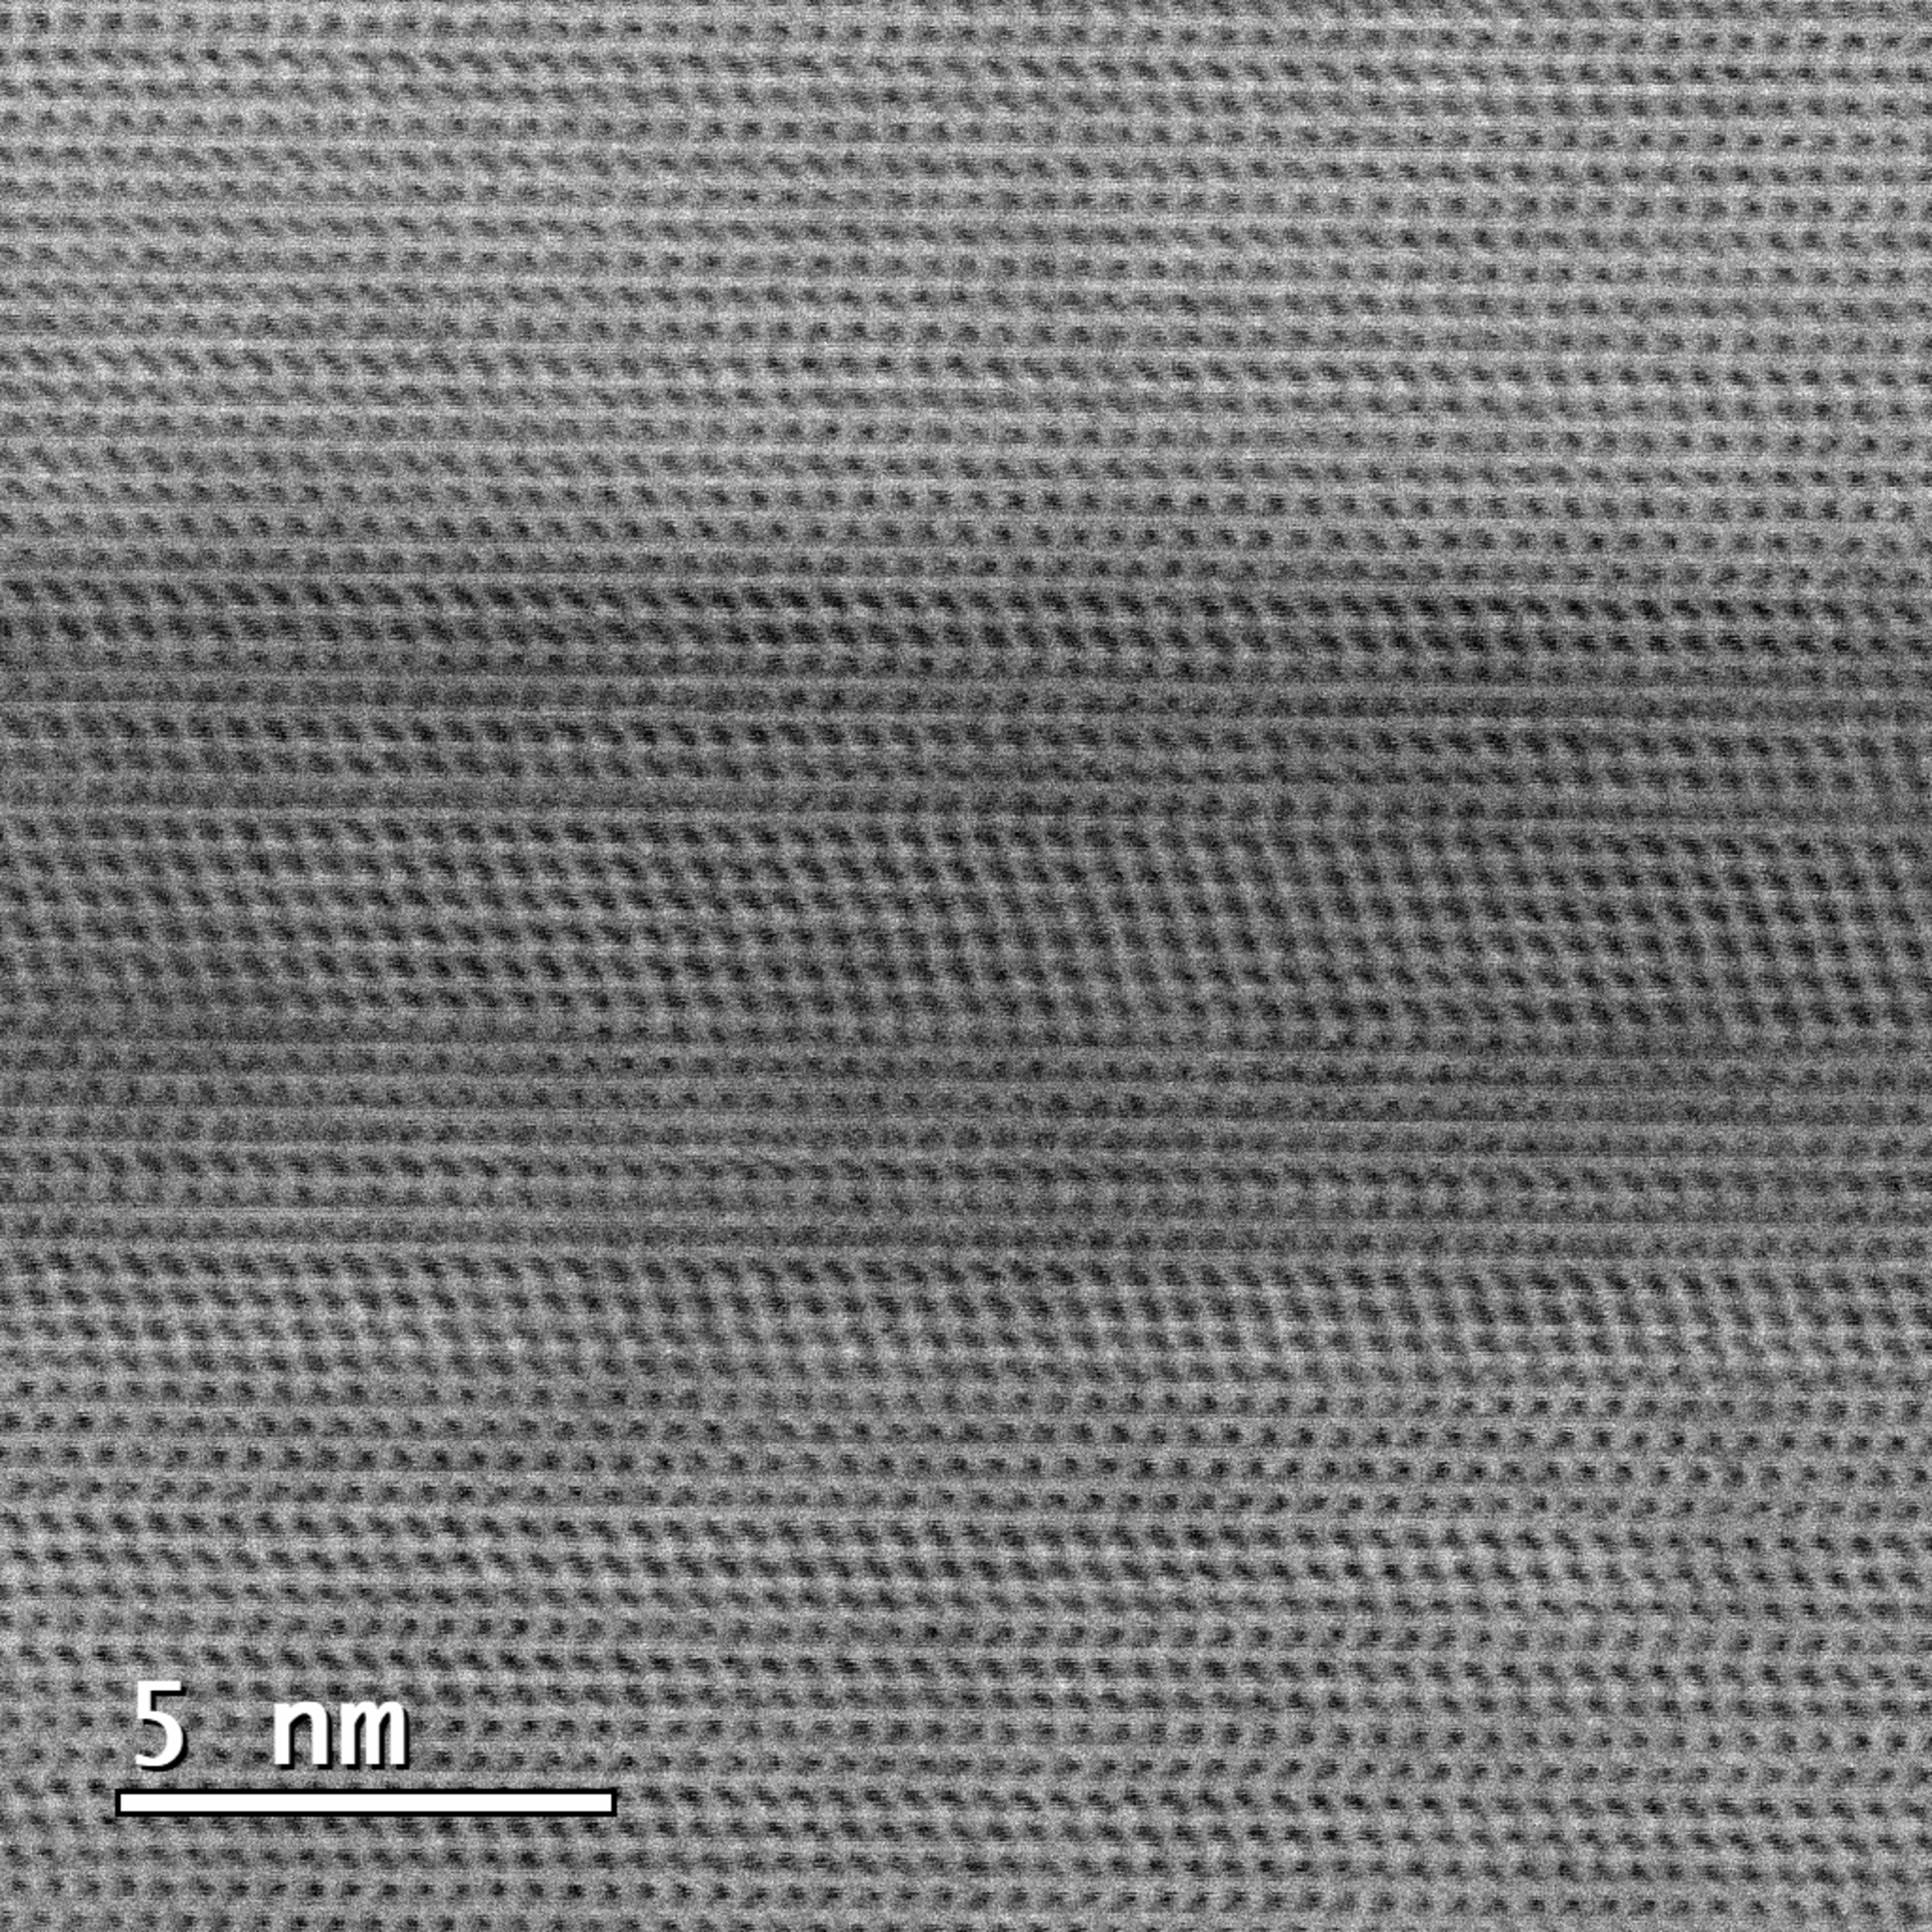
\includegraphics[width=0.48\textwidth]{4_Properties/Fig/merge_qw.pdf}
    }
    \caption{High resolution microscopy images for lattice analysis. \subref{subfig:merge_region} shows a \acs{df}-\acs{tem_m} image the region immediately after one of the spacers between the seed areas (visible in the bottom right of the image). \subref{subfig:merge_qw} shows a high-resolution \acs{bf}-\acs{tem_m} image of the first \acl{qw} (counting from the nucleation areas) in the common part of the template. \subref{subfig:merge_region} was kindly recorded by Michael Stiefel.}
    \label{fig:merge_high-res}
\end{figure}

Figure~\ref{subfig:merge_region} shows a magnified \acs{bf}-\acs{tem_m} image of the area immediately after the \acs{sio2} separation between the nucleation regions 2 and 3 marked in Figure~\ref{subfig:STEM_merge_structure_ov}. These \acs{tem_m} images make structural information readily available highlighting 1D and 2D defects better than their \acs{stem_m}-generated counterparts. This is evident in Figure~\ref{subfig:merge_region} by the presence of a series of lines delining many of the \hkl{1 1 1} planes in the III-V crystals. These lines are found in correspondence with \acs{rtp}s, which have been a common defect in all samples grown with the \hkl{1 1 1} growth front stabilisation method so far. The absence of other off-plane features in the image suggests the absence of other defects. However, a few defects could still be "hidden" because of the viewing angle.

A step-flow growth regimen can explain the absence of detectable defects on the merged regions between the three crystals \cite{Brugnolotto2023_2}. Under these growth conditions, each \acs{inp} atomic bilayer fills the width of the template before the next bilayer grows. This is the extreme result of the higher growth rates observed in \hkl<1 1 0> directions. In such a regimen, even if a crystal reached the larger template portion with the advantage of a few bilayers over the other two, its growth would support and be supported by the lattice matched \hkl{1 1 1} surfaces of the other two crystals. In this situation, as the leading crystal reaches the end of its individual seed area, diffusion of adsorbate atoms and precursors on the tightly packed \hkl{1 1 1} surface would bring precursors toward neighbouring wires. In such a configuration, the growth of shorter wires could be enhanced by the additional supply of precursors from the lead wire, up to the point where the \hkl{1 1 1} surface of the shorter wire can function as a support for the lateral expansion of the leading wire. Another option is for the leading wire to simply spill over the spacer: this situation would see the formation of non-\hkl{1 1 1} facets, which would quickly grow out, filling the neighbouring templates using the lattice-matched \acs{inp} crystals as support.

Once the single growth front is established, the growth of the crystal can continue under its step flow condition, creating the single-facet heterointerfaces seen in Figure~\ref{subfig:STEM_merge_structure_ov}. The high-resolution \acs{bf}-\acs{stem_m} image in Figure~\ref{subfig:merge_qw} shows a section of the first \acs{ingaas} \acl{qw}, counting from the nucleation areas toward the opening of the template. The \acs{rtp}s highlighted in the \acs{bf}-\acs{tem_m} image of Figure~\ref{subfig:merge_region} are identifiable by the apparent change of orientation of the biatomic units visible in this atomic resolution image. The heterostructure itself appears well-defined, on par with those of previous single nucleation samples on the \hkl<1 1 0> substrate shown in Figure~\ref{subfig:s4_HR}. 

\begin{table}
    \centering
    \caption{Growth rates for the superlattice region of the sample containing merge structures.}
    \begin{tabular}{c|c c c|c c c}
       & \multicolumn{3}{c}{\acs{ingaas}} & \multicolumn{3}{|c}{\acs{inp}} \\
       material layer & well 1 & well 2 & well 3 & barrier 1 & barrier 2 & barrier 3 \\ \hline
       growth rates (\nmmin) & \num[separate-uncertainty=true]{45 (3)} & \num[separate-uncertainty=true]{48 (2)} & \num[separate-uncertainty=true]{53 (3)} & \num[separate-uncertainty=true]{30.5 (0.3)} & \num[separate-uncertainty=true]{33.3 (0.3)} & \num[separate-uncertainty=true]{37.7 (0.3)} \\ \hline \hline
    \end{tabular}
    \label{tab:merge_growth_rates}
\end{table}

\paragraph{Growth rate} Table~\ref{tab:merge_growth_rates} shows the growth rates of each material layer starting at the first \acs{ingaas} \acl{qw} for the merge structure shown in Figure~\ref{subfig:STEM_merge_structure_ov}. This III-V structure was grown in the same growth run as the wire in Figure~\ref{subfig:s5_OV}, allowing a direct comparison to be drawn. The growth rates for the superlattice layers of the merge structure are higher compared to their single-seed counterparts. This can be explained by the difference in the size of the template, which is \qty{400}{\nano\metre} wide in the common section of the merge structure, while the nanowire in Figure~\ref{subfig:s5_OV} had a width of \qty{210}{\nano\metre}. Growth rates increase as the heterolayers grow closer to the opening of the template.

\section{Growth of Thin Heterolayers}

\begin{sidewaysfigure}
    \centering
    \subcaptionbox{
    Growth recipe for sample 6 \cite{Brugnolotto2023_2}. Each line represents an active flow of the corresponding precursor into the reactor. The colour of the horizontal lines represents the target material. The dashed lines are time-compressed 10 times. The \acl{qw} growth loop was executed six times.
    \label{subfig:recipe6}
    }{
        \tikzsetnextfilename{recipe6}
        \begin{tikzpicture}
        \begin{scope}
    % lines
            \node [label={[label distance=0]180:\acs{in}}] at (0, 0) {};
            \draw [cb1_orange, ultra thick] (0, 0) -- (1, 0); 
            \draw [cb1_dark_blue, ultra thick, dashed] (1, 0) -- (7, 0); %10
            \draw [cb1_orange, ultra thick] (9, 0) -- (9.5, 0);
            \draw [cb1_dark_blue, ultra thick, dashed] (11.2, 0) -- (12.2, 0); %10
        
            \node [label={[label distance=0]180:\acs{ga}}] at (0, -0.5) {};
            \draw [cb1_orange, ultra thick] (0, -0.5) -- (1, -0.5cm); 
            \draw [cb1_orange, ultra thick] (9, -0.5) -- (9.5, -0.5);
        
            \node [label={[label distance=0]180:\acs{as}}] at (0, -1) {};
            \draw [cb1_orange, ultra thick] (0, -1) -- (1, -1); 
            \draw [cb1_orange, ultra thick] (9, -1) -- (9.5, -1);
            \draw [gray, ultra thick] (9.5, -1) -- (10.2, -1);
        
            \node [label={[label distance=0]180:\acs{p}}] at (0, -1.5) {};
            \draw [cb1_dark_blue, ultra thick, dashed] (1, -1.5) -- (7, -1.5); %/10
            \draw [gray, ultra thick] (7, -1.5) -- (9, -1.5);
            \draw [gray, ultra thick] (10.2, -1.5) -- (11.2, -1.5);
            \draw [cb1_dark_blue, ultra thick, dashed] (11.2, -1.5) -- (12.2, -1.5); %/10
            \draw [gray, ultra thick] (12.2, -1.5) -- (14.2, -1.5);
        
    % labels and markers for the timescale
            \node [label={[label distance=0]180:Time (\second)}] at (0, -2) {};
            \draw [] (0, -2) -- (1, -2);
            \draw [dashed] (1, -2) -- (7, -2);
            \draw [] (7, -2) -- (11.2, -2);
            \draw [dashed] (11.2, -2) -- (12.2, -2);
            \draw [-stealth] (12.2, -2) -- (14.5, -2); % +0.3
            \draw [] (0, 0.2) -- (0, -2.2) node[anchor = north] {\num{0}};
            \draw [] (1, 1.2) -- (1, -2.2) node[anchor = north] {\num{10}};
            \draw [] (7, 0.2) -- (7, -2.2) node[anchor = north] {\num{610}};
            \draw [] (9, 0.4) -- (9, -2.2) node[anchor = north] {\num{630}};
            \draw [] (9.5, 0.2) -- (9.5, -2.8) node[anchor = north] {\num{635}};
            \draw [] (10.2, 0.2) -- (10.2, -2.2) node[anchor = north] {\num{642}};
            \draw [] (11.2, 0.2) -- (11.2, -2.2) node[anchor = north] {\num{652}};
            \draw [] (12.2, 0.2) -- (12.2, -2.2) node[anchor = north] {\num{752}};
            \draw [] (14.2, 1.2) -- (14.2, -2.2) node[anchor = north] {\num{772}};
            \draw [stealth - stealth] (9, 0.3) -- (14.2, 0.3) node[midway, anchor=south] {Quantum Well Loop (x\num{6})};
            \draw [stealth - stealth] (1, 1.1) -- (14.2, 1.1) node[midway, anchor=south] {Deposition Loop (x\num{2})};
        \end{scope}
        \begin{scope} [shift={(15.4cm, -0.5)}] % +0.9
            \draw [gray, ultra thick] (0, 0.5) -- (0.5, 0.5) node[anchor = west, text=black] {Hold Step};
            \draw [cb1_orange, ultra thick] (0, 0) -- (0.5, 0) node[anchor = west, text=black] {\acs{ingaas}};
            \draw [cb1_dark_blue, ultra thick] (0, -0.5) -- (0.5, -0.5) node[anchor = west, text = black] {\acs{inp}};
            \draw [dashed, ultra thick] (0, -1) -- (0.5, -1) node[anchor = west, text = black] {\num{0.1} time scale};
            \draw (-0.3, 1) -- (3.3, 1) -- (3.3, -1.65) -- node[midway, fill = white] {Legend} (-0.3, -1.65) -- cycle;
        \end{scope}
        \end{tikzpicture}
    }
     \subcaptionbox{
        \acs{bf}-\acs{stem_m} image of a nanowire grown with the recipe in \subref{subfig:recipe6} \cite{Brugnolotto2023_2}. Each material layer is labelled, and a guide highlighting the lattice rotation is present.
        \label{subfig:s6_wire_OV}
    }{
        \tikzsetnextfilename{s6_wire_OV}
        \begin{tikzpicture}
            \node[inner sep=0pt] (image) at (0,0) {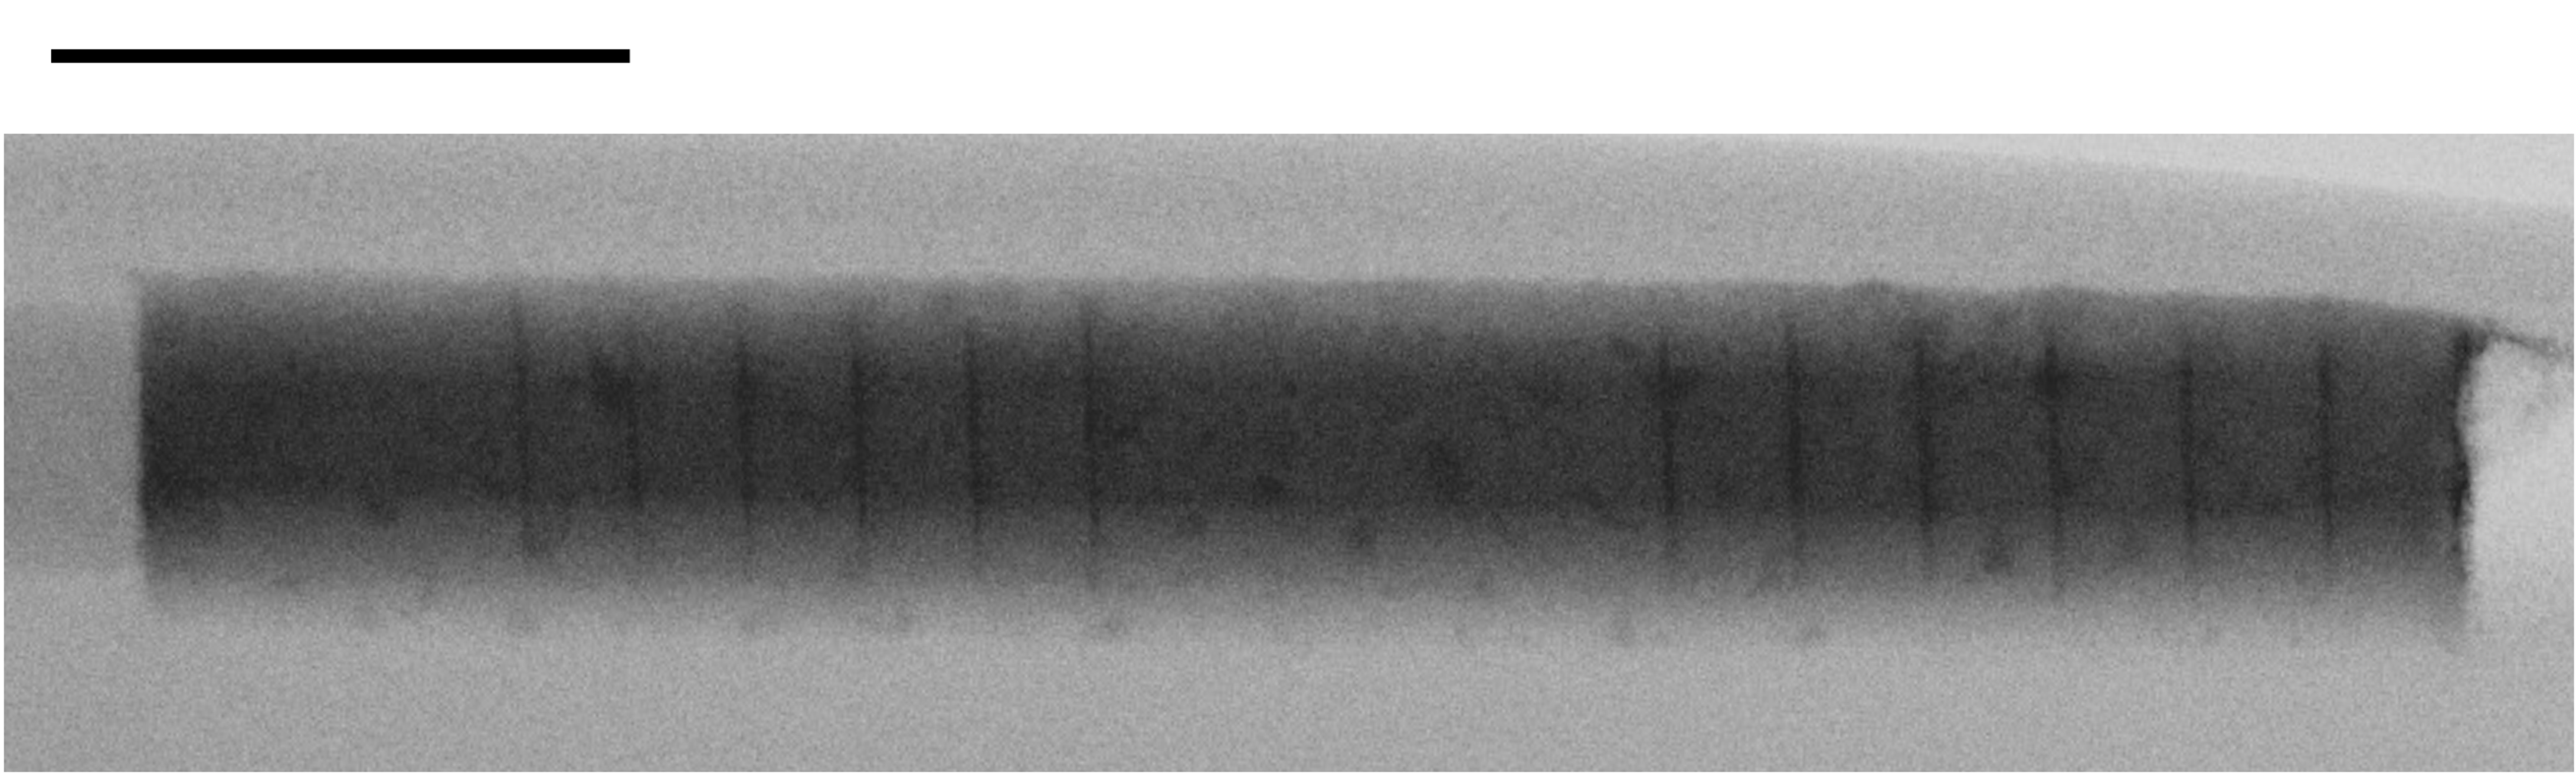
\includegraphics[width=\textwidth]{4_Properties/Fig/s6_wire_ov.pdf}};
            \node at (-10.7, 2.8) {\qty{200}{\nano\metre}};
            \node[white] at (-11.5, 1.7) {\acs{sio2}};
            \draw[white, decorate, decoration={brace, mirror}] (-1.8, 1.1) -- (-7.4, 1.1) node[midway, anchor=south]{\num{6}x \acs{ingaas} \acl{qw}s};
            \draw[white, decorate, decoration={brace, mirror}] (10, 1.1) -- (3.4, 1.1) node[midway, anchor=south]{\num{6}x \acs{ingaas} \acl{qw}s};
            \node[white] at (-11.5, -0.5) {\acs{si}};
            \node[white] at (0, -0.5) {\acs{inp}};
            \node[white] at (-11.5, -2.5) {\acs{sio2}};
            \draw[white] (-7.14, -2) -- (-10.85, -2) -- (-10.85, -1);
            \draw[white] (-10.85, -1.5)  -- ++ (0.5, 0) node[anchor=south west]{\qty{90}{\degree}} -- ++ (0, -0.5);
            \draw[white] (-7.65, -2) arc [start angle = 180, end angle = 93, radius = 0.5] node[midway, anchor=south east]{\qty{87}{\degree}};
            \draw[white] (-7.2, -1) -- ++ (-87:1);
            \path[decorate, decoration={text along path, text color = red, text={EDS linescan},text align=center}] (3,-0.5) -- ++ (3:7.5);
            \draw[red, -stealth] (3,-0.8) -- ++ (3:7.5);
        \end{tikzpicture}
    }
    \caption{\acs{mocvd} growth recipe \subref{subfig:recipe6} and resulting nanowire \subref{subfig:s6_wire_OV} for sample 6.}
    \label{fig:s6_recipe+OV}
\end{sidewaysfigure}

A modified growth recipe was built based on the results of sample 5. The main objectives were to create even thinner \acs{ingaas} \acl{qw}s, which would give more information on the minimum thickness of the heterolayer achievable by \acs{mocvd} growth using the facet stabilisation method and a further decrease of the post-\acs{ingaas} \acl{as} hold step, to try to further mitigate the \acl{as} contamination in the \acs{inp} region immediately after each \acl{qw}.

The resulting recipe is shown in Figure~\ref{subfig:recipe6}. The \acs{ingaas} nucleation layer's deposition time was decreased from \qty{30}{\second} to \qty{10}{\second}. As there had been no nucleation issues with the \qty{30}{\second} deposition time in sample 5, a lower step time was tested for this sample to minimise the amount of \acs{ingaas} outside the \acl{qw}s. The recipe segments and loops following the nucleation layer were run twice. After \qty{600}{\second} of \acs{inp} growth, the deposition of the \acs{ingaas}/\acs{inp} superlattice took place. The step time for \acs{ingaas} was reduced from \qty{10}{\second} to \qty{5}{\second}, and the post-\acs{ingaas} \acl{as} hold step shortened from \qty{10}{\second} to \qty{7}{\second}. The deposition times of the barrier layers were also shortened from \qty{200}{\second} to \qty{100}{\second}. The number of repetitions of the \acl{qw} loop was doubled from \num{3} to \num{6}. The cumulative changes were meant to double the number of \acl{qw}s present in the same length of nanowires that contained the superlattice in sample 5, while repeating the entire recipe twice was meant to result in a longer overall nanowire to highlight differences in growth rate based on the depth of each material layer in the template.

The \qty{30}{\degree} cross-section of a nanowire grown with this revised recipe is shown in the \acs{bf}-\acs{stem_m} image in Figure~\ref{subfig:s6_wire_OV}. The angled view given by this tilted cross-section causes the shaded top and bottom interfaces of the III-V material region. The circular shades in the image are given by indium droplets, a common residue left over from \acs{fib} lamella preparation. The III-V material, appearing darker in the centre of the image, is sandwiched between the template oxide at the top and the buried oxide layer at the bottom. The \acs{si} seed is visible on the left of the image, while the \acs{ingaas} nucleation layer is too thin to appear as more than a darker shade at the very beginning of the nanowire. Twelve vertical lines, darker compared to the \acs{inp} making up the majority of the wire, are created by a change in channelling contrast given by the presence of \acl{as} atoms, which are larger than the \acl{p} atoms that make up the majority of the V element atoms in the wire.

The seed surface consists of a single \hkl{1 1 1} facet resulting from the selective etching of \acs{si} carried out with \acs{tmah} before deposition. This surface forms a \qty{90}{\degree} angle with the wafer plane, but, as can be seen in the highlight in Figure \ref{subfig:s6_wire_OV}, the first \acl{qw}, and indeed all the others, are tilted \qty{3}{\degree} off the perpendicular to the wafer plane. A slight rotation of the growing lattice compared to the seed's lattice orientation can occur during epitaxy because it is a way for the growing crystal to compensate for some of the stress caused by lattice mismatch. Despite the \qty{3}{\degree} rotation, the stabilisation of the \hkl{1 1 1} facet is achieved during the initial \acs{inp} deposition and is maintained throughout the wire. The \num{12} \acl{qw}s range in thickness from \qty{3.7}{\nano\metre} to \qty{4.3}{\nano\metre}.

\begin{figure}
    \centering
    \subcaptionbox{
        \acs{bf}-\acs{stem_m} image of the \acs{si} / III-V interface.
        \label{subfig:s6_si-IIIV_interface}
    }{
        \tikzsetnextfilename{s6_si-IIIV_interface}
        \begin{tikzpicture}
            \node[inner sep=0pt] (image) at (0,0) {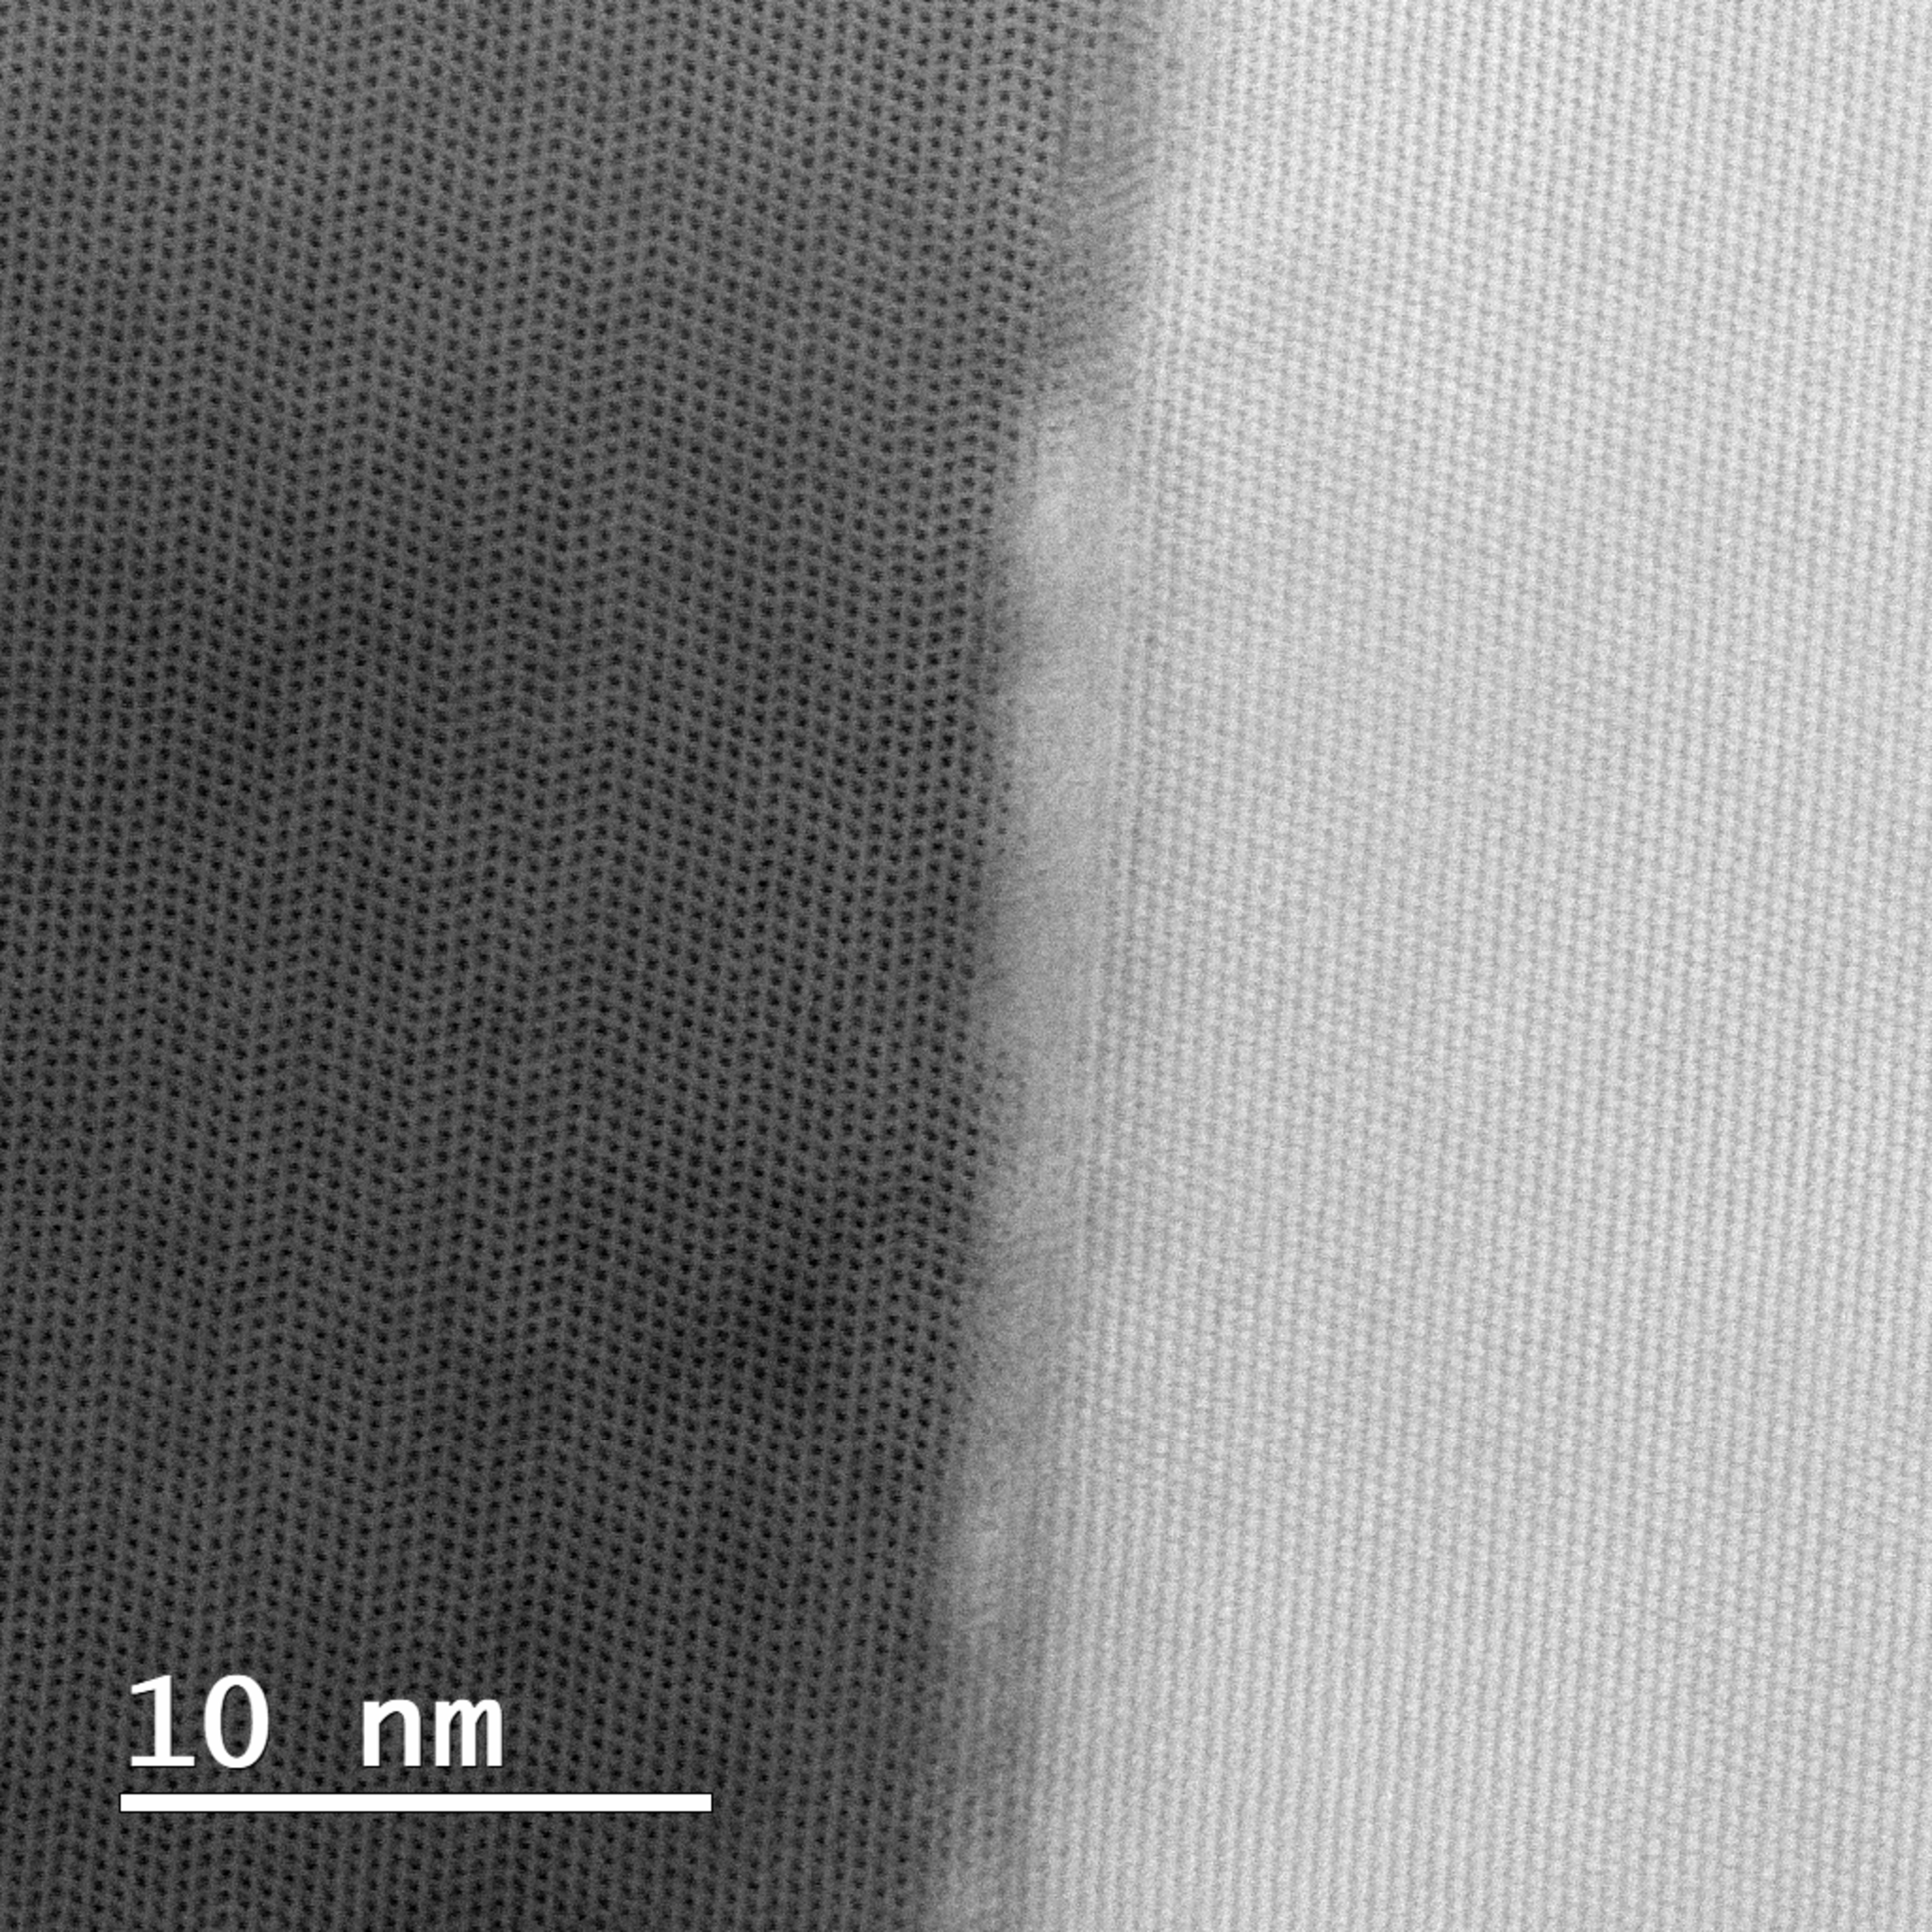
\includegraphics[width=0.48\textwidth]{4_Properties/Fig/s6_si-IIIV_interface.pdf}};
            \draw [red] (0.19, 3.85) -- ++ (-95.3:7.7) -- ++ (0:1.5) -- ++ (86:7.7);
            \draw [red] (0.28, 3.85) -- ++ (-95.3:7.7);
            \draw [red] (0.36, 3.85) -- ++ (-95.3:7.7);
            \draw [red] (0.44, 3.85) -- ++ (-95.3:7.7);
            \draw [red] (0.53, 3.85) -- ++ (-95.3:7.7);
            \draw [red] (0.61, 3.85) -- ++ (-95.3:7.7);
            \draw [red] (0.69, 3.85) -- ++ (-95.3:7.7);
            \draw [red] (0.77, 3.85) -- ++ (-95.3:7.7);
        \end{tikzpicture}
    }
    \subcaptionbox{
        \acs{bf}-\acs{stem_m} image of the first \acs{ingaas} \acs{qw}.
        \label{subfig:s6_well1}
    }{
        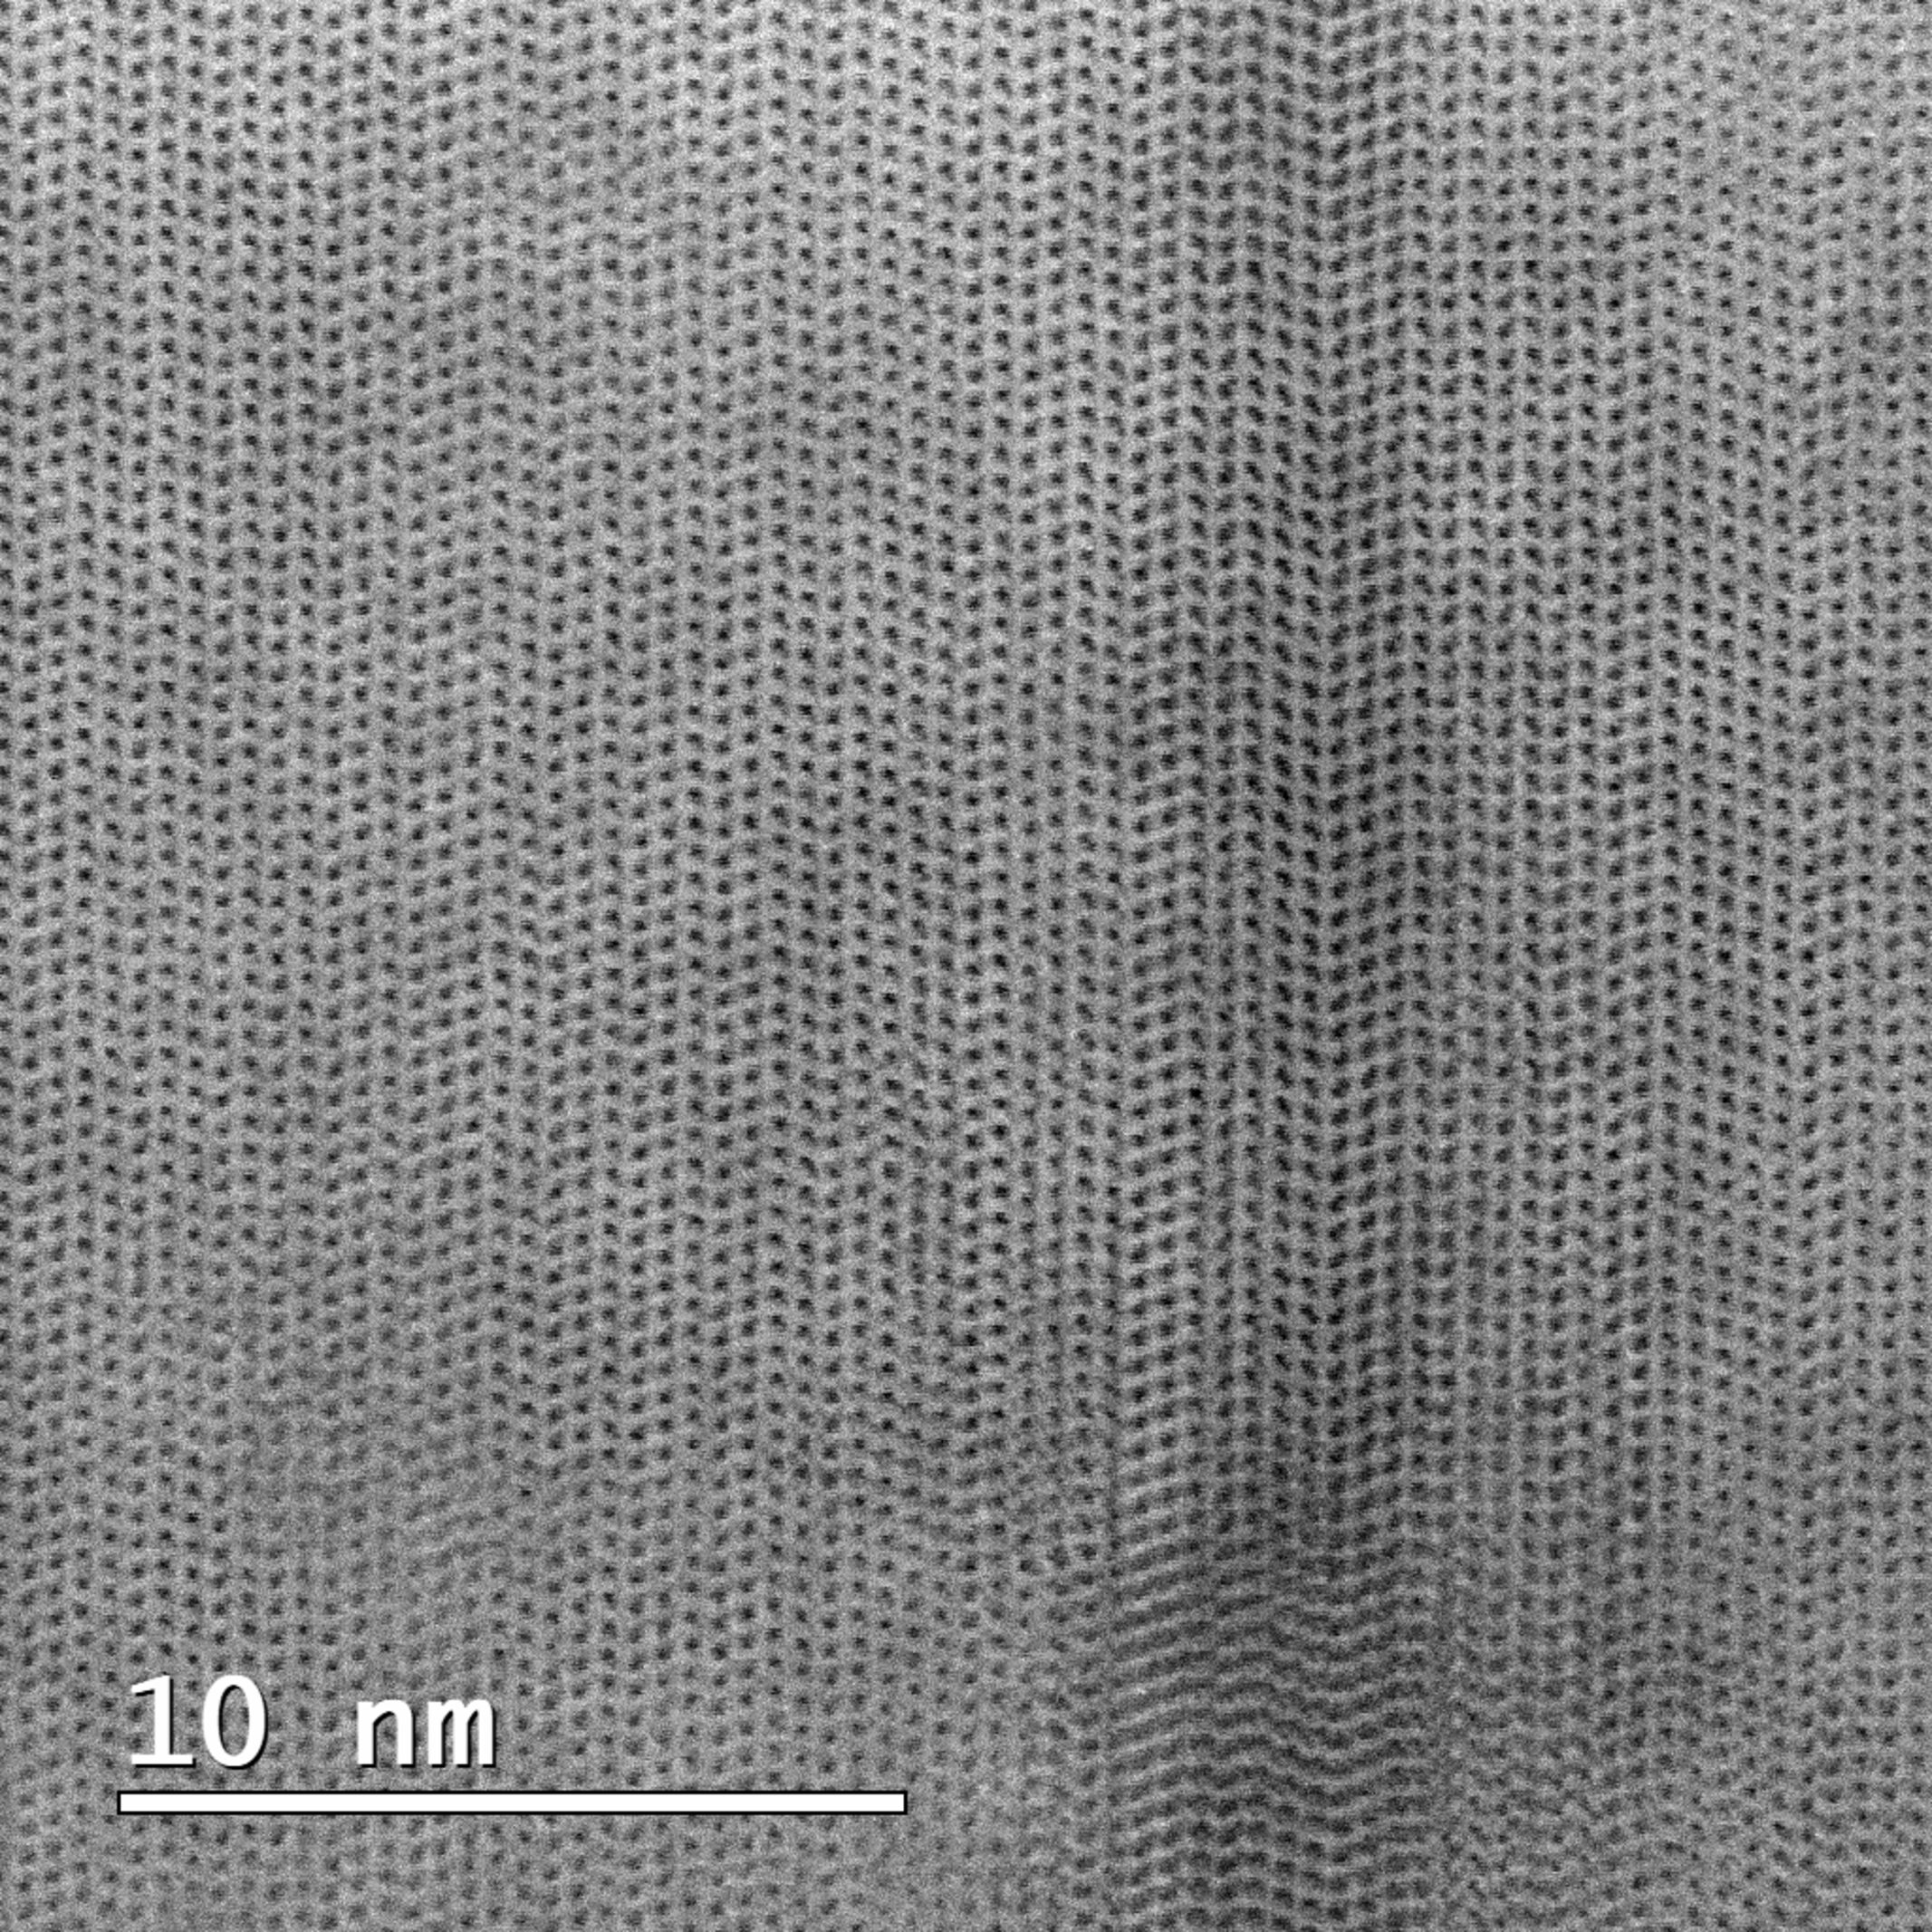
\includegraphics[width=0.48\textwidth]{4_Properties/Fig/s6_well1.pdf}
    }
    \caption{High-resolution \acs{bf}-\acs{stem_m} images of \subref{subfig:s6_si-IIIV_interface} the nucleation area, showing the \acs{si} / \acs{ingaas} hetyerointerface, and of \subref{subfig:s6_well1} the first \acl{qw} in sample 6.}
    \label{fig:s6_HR}
\end{figure}

\paragraph{High resolution analysis} Figure~\ref{fig:s6_HR} shows high resolution \acs{bf}-\acs{stem_m} images of two heterostructures in the nanowire seen in Figure~\ref{subfig:s6_wire_OV}. Many \acs{rtp}s are present in both images, confirming that this defect is the most common in III-V \(_B\) growth on \hkl{1 1 1}\(_B\) planes. 

Figure~\ref{subfig:s6_si-IIIV_interface} shows the heterointerface between the \acl{si} seed and the \acs{ingaas} nucleation layer. \num{8} red lines were added parallel to the first visible continuous biatomic layer on the \acs{ingaas} side. A single red line was added to follow one of the \acs{si} \hkl{1 1 1} facets. By comparing the distance between the lines at the top and bottom of the image, it is clear that the two lattices are already misaligned at the nucleation interface. This region is strained by the mismatch between two lattices, and the first few \acs{ingaas} atomic layers after the \acs{si} seed surface are prone to nucleation for dislocations. The presence of this type of defect in the blurred area at the centre of the image can explain the varying distance between the two \hkl{1 1 1} atomic planes in the \acs{ingaas} and \acs{si}.

The first, counting from the \acs{si} seed, \acs{ingaas} \acl{qw} appears as the darker vertical stripe in Figure~\ref{subfig:s6_well1}. The well is well-defined thanks to the channelling contrast between the light \acl{p} atoms and the heavier \acs{as} atoms, which denotes a good segregation of the two species in the respective layers. Comparing the \acs{inp} layers at either side of the well, however, shows a darker shade on the right, in the \acs{inp} area, which grew immediately after the \acs{ingaas} heterolayer. This suggests the presence of \acl{as} contamination after the well, as observed in all previous samples.
\par

\begin{figure}
    \centering
    \tikzsetnextfilename{s6_growth_rates}
    \begin{tikzpicture}
        \begin{axis}[%
            width = 0.8\textwidth,
            height = 6cm,
            xlabel = Position (nm),
            ylabel = Growth Rates (\nmmin),
            table/col sep=semicolon,
            error bars/y dir = both, 
            error bars/y explicit,
            error bars/x dir = both, 
            error bars/x explicit,
            legend pos=outer north east,
        ]
        \addplot [cb1_dark_blue,
                only marks,
                /pgf/number format/read comma as period,
                ] 
                table[
                        x=Position,
                        y=Barrier Growth Rate,
                        x error = P_err,
                        y error = BG_err
                        ] {4_Properties/csv/barrierGR.csv};
        \addlegendentry{InP Barrier }
        \addplot [cb1_orange,
                only marks,
                /pgf/number format/read comma as period,
                ] 
                table[
                        x=Position,
                        y=Well Growth Rate,
                        x error = P_err,
                        y error = WG_err
                        ] {4_Properties/csv/barrierGR.csv};
        \addlegendentry{InGaAs Well}
        \end{axis}

    \end{tikzpicture}
    \caption{\acs{ingaas} and \acs{inp} material layer growth rates as a function of their distance from the \acs{si} seed surface \cite{Brugnolotto2023_2}. Both x and y error bars are present but smaller than the markers, except for those on the growth rate of \acs{ingaas}.}
    \label{fig:s6_growth_rates}
\end{figure}

\paragraph{Growth rate} Growth rates in the \acl{qw} structure were calculated by averaging seven thickness measurements of each material layer along the \hkl<1 1 1> direction and dividing them by the deposition time, which is taken from the recipe and is assumed to be error-free. Figure~\ref{fig:s6_growth_rates} shows each growth rate as a function of the distance of the first heterointerface of the respective layer from the \acs{si} seed. This metric is also calculated by averaging seven measurements and errors on the first heterointerface's position and the growth rates of each layer to express the \qty{95}{\%} confidence interval. All errors were plotted in Figure~\ref{fig:s6_growth_rates}. However, the only error bars that exceeded the size of the graph markers were those of the \acs{ingaas} \acl{qw} growth rates.

Growth rates for \acs{inp} layers start at \qty[separate-uncertainty=true]{20.8 (0.5)}{\nano\metre\per\minute} and end at \qty[separate-uncertainty=true]{26.2 (0.2)}{\nano\metre\per\minute}, falling between those of samples 4 and 5. On the other hand, the growth rates of \acs{ingaas} \acl{qw}s is higher than both those of samples 4 and 5 and ranges from \qty[separate-uncertainty=true]{41 (3)}{\nano\metre\per\minute} to \qty[separate-uncertainty=true]{52 (4)} {\nano\metre\per\minute}. The increase in the growth rate values with the nearing of the growth front to the opening of the template confirms its dependence on the diffusion process of the precursors and adsorbates in the template \cite{bjork2012}. Their lower thickness gives the higher error in the growth rates of the \acs{ingaas} layers.

\begin{figure}
    \centering
    \subcaptionbox{
    \acs{eds} linescan: III atomic percentage vs position.
    \label{subfig:s6_III_30deg_linesc}
    }{
    \tikzsetnextfilename{s6_III_30deg_linesc}
    \begin{tikzpicture}
        \begin{axis}[
            width = 0.8\textwidth,
            height = 5cm,
            xlabel = Position (nm),
            ylabel = Composition (atomic \%),
            table/col sep=comma,
            %title = III element composition,
            legend pos=outer north east,
            ymin=0, ymax=100,
            xmin = 0, xmax=294.3
        ]
    \addplot [cb1_orange,] table[x=nm,y=Ga] {4_Properties/csv/s6_III_30deg_linesc.csv};
    \addplot [cb1_dark_blue,] table[x=nm,y=In] {4_Properties/csv/s6_III_30deg_linesc.csv};
    \addlegendentry{Ga}
    \addlegendentry{In}
    \end{axis}

    \end{tikzpicture}
    }
    \subcaptionbox{
    \acs{eds} linescan: V atomic percentage vs position.
    \label{subfig:s6_V_30deg_linesc}
    }{
    \tikzsetnextfilename{s6_V_30deg_linesc}
    \begin{tikzpicture}
        \begin{axis}[
            width = 0.8\textwidth,
            height = 5cm,
            xlabel = Position (nm),
            ylabel = Composition (atomic \%),
            table/col sep=comma,
            %title = V element composition,
            legend pos=outer north east,
            ymin=0, ymax=100,
            xmin = 0, xmax=294.3
        ]
    \addplot [cb1_orange,] table[x=nm,y=As] {4_Properties/csv/s6_V_30deg_linesc.csv};
    \addplot [cb1_dark_blue,] table[x=nm,y=P] {4_Properties/csv/s6_V_30deg_linesc.csv};
    \addlegendentry{As}
    \addlegendentry{P}
    \end{axis}

    \end{tikzpicture}
    }
    \caption{\acs{eds} linescan compositional data (in percentage) for the \subref{subfig:s6_III_30deg_linesc} III elements and \subref{subfig:s6_V_30deg_linesc} V elements 
    across the last \num{6} \acl{qw}s of sample 6 (Figure~\ref{subfig:s6_wire_OV}). The origin of the x-axis is situated before the first well and is the closest point to the \acs{si} seed. Higher position numbers (in nm) represent the scan moving along the \hkl{1 1 1} vector perpendicular to the growth front away from the seed.}
    \label{fig:s6_30deg_linescans}
\end{figure}

\paragraph{\acs{eds} analysis} An \acs{eds} linescan was carried out along the \hkl<1 1 1> vector marked in red in Figure~\ref{subfig:s6_wire_OV}, which also defines the \hkl{1 1 1} single-facet heterointerfaces, to capture the variation in composition across the last \num{6} \acs{ingaas} \acl{qw}s. Figure~\ref{subfig:s6_III_30deg_linesc} shows the concentration profile of the III element. The noise level is around \qty{15}{\%} and the calculated atomic percentage of \acl{ga} in the \acs{ingaas} layer ranges from \qty{40}{\%} to \qty{50}{\%}. These concentrations are in line with those seen in Figure~\ref{subfig:s5_III_0deg_linesc} for sample 5.

Figure~\ref{subfig:s6_V_30deg_linesc}, however, shows a low \acl{as} concentration in the \acs{ingaas} layers. Its highest value is \qty{80}{\%} in well \num{9}, while it oscillates between \qty{50}{\%} and \qty{60}{\%} in wells \num{7}, \num{8}, \num{10}, \num{11}, and \num{12}. These concentration profiles depart from the very well-segregated V elements shown in Figure~\ref{subfig:s3_V_linesc}, \ref{subfig:s4_V_0deg_linesc}, and \ref{subfig:s5_V_0deg_linesc}. This indicates that layers under \qty{5}{\nano\metre} in thickness could be too thin to allow for a complete switch in composition from \acl{p} to \acs{as}. Other explanations involve probe size effects, which could be "smoothing" the composition profiles across the heterointerfaces, or a small angle in the lamella exposing both \acs{ingaas} and \acs{inp} to the beam. However, comparing the V-element profiles with the III-element profiles, it appears unlikely that either of these instrument-related distortions could have played a major role. Indeed, the same effects would be expected to affect the concentration profile of the III elements, lowering the \acl{ga} concentration as a result. The fact that this has not happened makes the possibility that the thickness of the transition layer is on the order of \qty{2}{\nano\metre} more likely.

\Acl{as} contamination continues to be present in the \acs{inp} layer immediately after the \acs{ingaas} \acl{qw}s.

\subsection{Growth in a competitive environment}

\begin{figure}
    \centering
    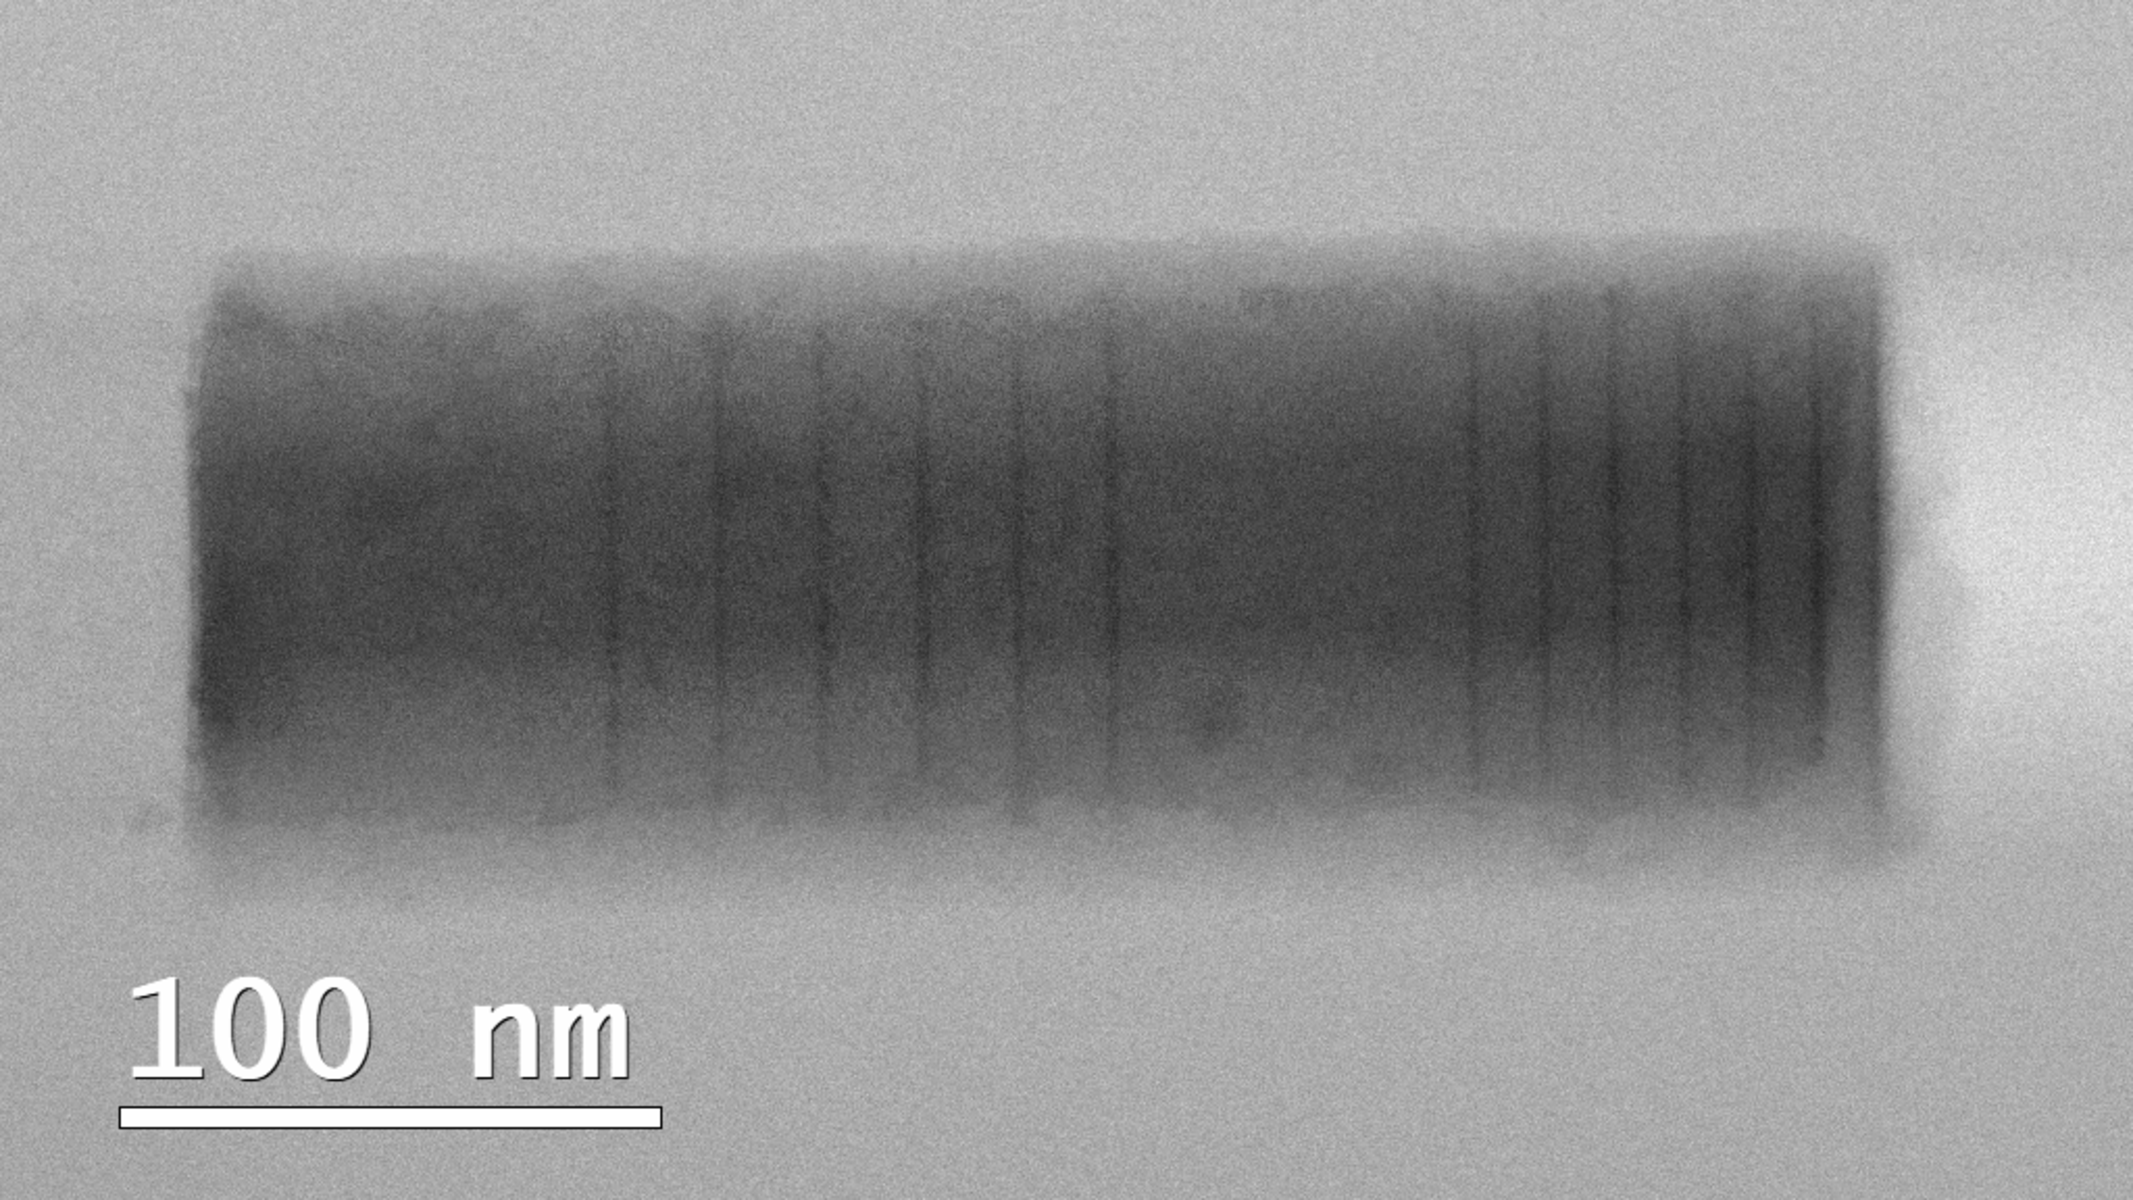
\includegraphics[width=\textwidth]{4_Properties/Fig/s6_competitive_OV.pdf}
    \caption{\acs{bf}-\acs{stem_m} image of a nanowire from sample 6 grown in an area of the wafer with many parasitic nucleations.}
    \label{fig:s6_competitive_OV}
\end{figure}

As seen in the \acs{sem_m} image in Figure~\ref{subfig:SEM_array}, competition between multiple nucleation points within a nanowire array does not result in a pronounced variation of growth rate within the nanowires. 

Figure~\ref{fig:s6_competitive_OV} shows a nanowire grown in an area of the wafer with many parasitic crystals. This can happen because of leftover contaminants on the wafer surface. In this case, the contaminants were likely deposited by vacuum-driven evaporation of a small droplet left on the surface of the chip after manipulation with wet tweezers. The contaminants act as additional nucleation centres for the III-V precursors. This is similar to the procedure used to create a self-assembled distribution of nanocrystals. The resulting \qty{100}{\nano\metre}-wide crystals created a much more competitive growth environment compared to the rest of the chip that was unaffected by this issue and from which the wire in Figure~\ref{subfig:s6_wire_OV} was cut.

As a result, the wire in Figure~\ref{fig:s6_competitive_OV} is considerably shorter than the wire in Figure~\ref{subfig:s6_wire_OV}. The \acs{ingaas} nucleation step resulted in a nanocrystal visible by channelling contrast in the lower left portion of the \acs{si} / III-V interface. The \num{12} \acs{ingaas} \acl{qw}s are still visible in the \acs{inp} matrix and provide a snapshot of the evolution of the growth front. Counterintuitively, the growth rates of the various heterolayers appear to decrease as the wire grows towards the opening of the template, as demonstrated by the shorter \acs{inp} segments in the last part of the wire. 

As parasitic crystals grow, so does their ability to capture precursors. As a result of the template oxide restricting the gas phase diffusion of the precursors to a smaller solid angle and lengthening the surface diffusion distance the adsorbates have to travel to reach the growing nanowire, the precursor capturing power of the parasitic crystals increases more rapidly than that of the \acs{tase} nanowires. This competition mechanism explains the decrease in the growth rate of the nanowire. Further, the last \acs{ingaas} \acl{qw} of the wire in Figure~\ref{fig:s6_competitive_OV} is shorter than the others, with a multi-facet growth front forming in the previous \acs{inp} barrier layer. This indicates that the effective V/III ratios in the template are beginning to be affected by the competitivity of the parasitic crystals in precursor capture.

If the deposition of densely packed III-V structures is planned, the effect of this competition during \acs{mocvd} growth should be taken into account to ensure that the desired material properties are obtained.

\section{Growth of Strained Heterolayers}

All samples shown in this thesis so far targeted an \ce{In0_.53Ga0_.47As} composition in the arsenide layers, with varying degrees of success as resulting from \acs{eds} analysis. This composition is lattice matched to the supporting \acs{inp} barrier layer \cite{Pearsall1980, Sugii1983, Wagner1970}, therefore simplifying the 












\subsection{Arsenides and phosphides}
\paragraph{Strain analysis}
\subsection{Antimonides}

\section{Doped semiconductors}

\section{Discussion and future developments}







\section{article 2}
\subsection{Heterointerfaces and growth rate in nanowires}

%\begin{figure}
%     \centering
%     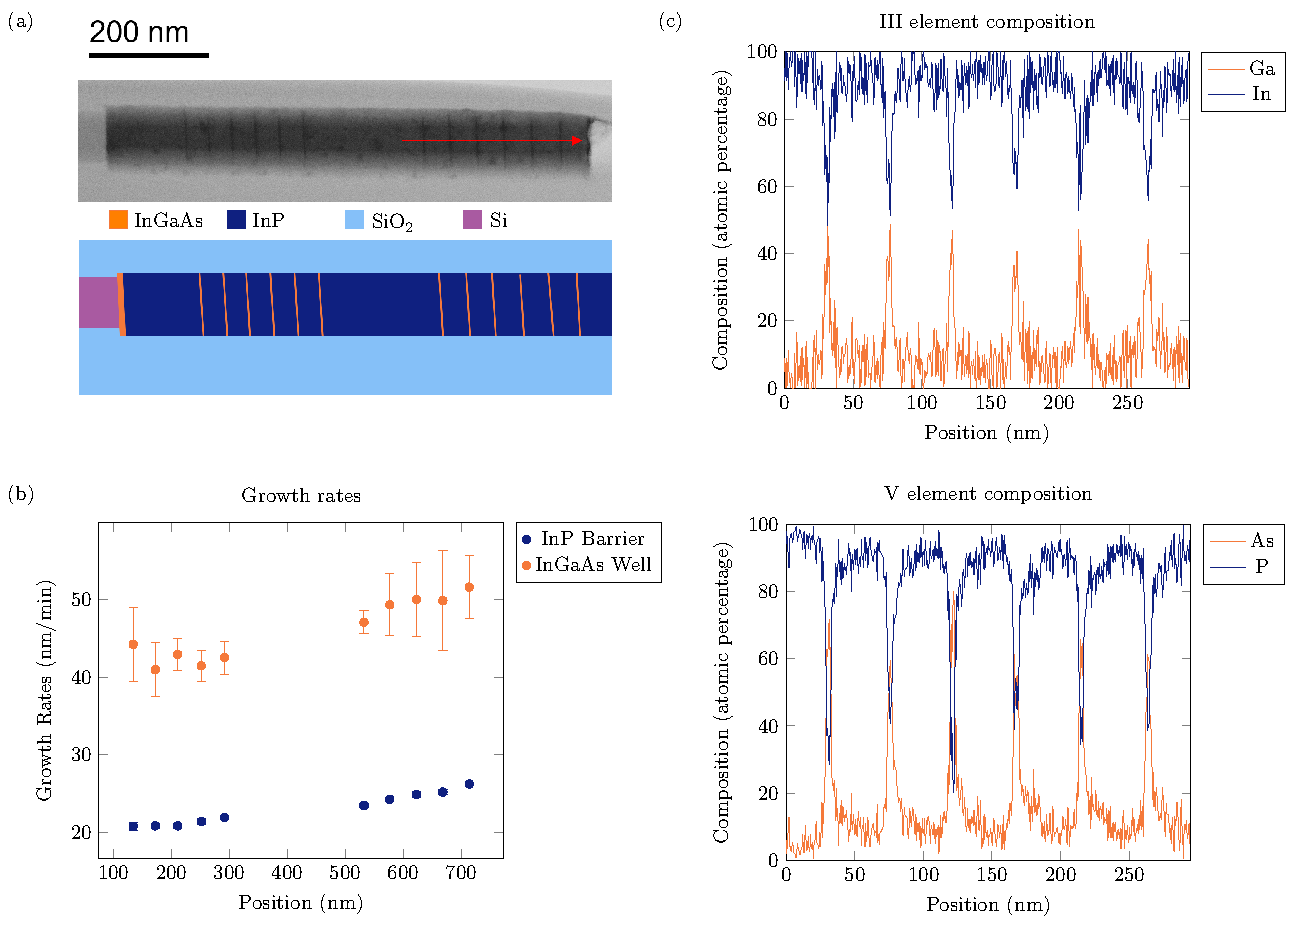
\includegraphics[width=\textwidth]{4_Properties/From_Article2/Figure4.pdf}
%     \caption{Characterisation results for sample 1. (a) BF-STEM image of the cross-section of one of the nanowires and corresponding schematic composition drawing. (b) growth rates of \acs{ingaas}, in orange, and \acs{inp}, in dark blue. Error bars on all x coordinates, and y coordinates of the \acs{inp} series, are smaller than the graphical markers. (c) composition profiles calculated from an EDS line scan recorded on the location and with the direction marked by the red arrow in (a).}
%     \label{fig:growth_rates}
% \end{figure}

%An in-depth STEM and EDS analysis was carried out to assess the structure of the nanowires. Figure~\ref{fig:growth_rates}.a shows the STEM microscopy image of a FIB cross-section of a wire from sample 1. The blurred regions at the top and bottom are due to the \qty{30}{\degree} cut angle employed to access the \hkl<110> imaging direction. 

%The \qty{4}{\nm} thin, on average, \acs{ingaas} segments are visible as twelve thin dark vertical lines in the dark grey body of the wire. 

%The \acs{ingaas} layers cross-section also act as time markers, recording the morphology of the growth front, and revealing when a single facet is formed and maintained in the growth process. 

%The slight tilt of the heterolayers, which do not appear to be perpendicular to the wafer surface, can partially be explained by a slight tilt of the device \acs{si} layer in this area of the wafer, as well as tilting due to a rotation of the crystalline growth axis during nucleation.

% An EDS line scan of the last six \acs{ingaas} quantum wells was recorded along the direction indicated by the red arrow in Figure~\ref{fig:growth_rates}.a. The resulting composition profiles are shown in Figure~\ref{fig:growth_rates}.c, demonstrating consistent composition profiles across the wells, with the \acs{in} molar fraction being between \num{0.5} and \num{0.6}.

%A growth rate analysis is shown in Figure~\ref{fig:growth_rates}.b, revealing a variation in the \acs{inp} growth rate of around \qty{6}{\nm\per\minute} from \qty[separate-uncertainty=true]{20.7 (0.5)}{\nano\metre\per\minute} to \qty[separate-uncertainty=true]{26.2 (0.2)}{\nano\metre\per\minute} along \qty{600}{\nm} of wire. Similarly, a \qty{7}{\nano\metre\per\minute} growth rate increase was recorded for the \acs{ingaas} segments. The error bars represent the \qty{95}{\%} confidence interval on the measurement, calculated by averaging seven thickness measurements taken at various positions for each \acs{inp} and \acs{ingaas} segment. This growth rate increase shows a moderate influence of the diffusional process on the growth dynamics of the samples \cite{bjork2012}.

\begin{figure}
    \centering
    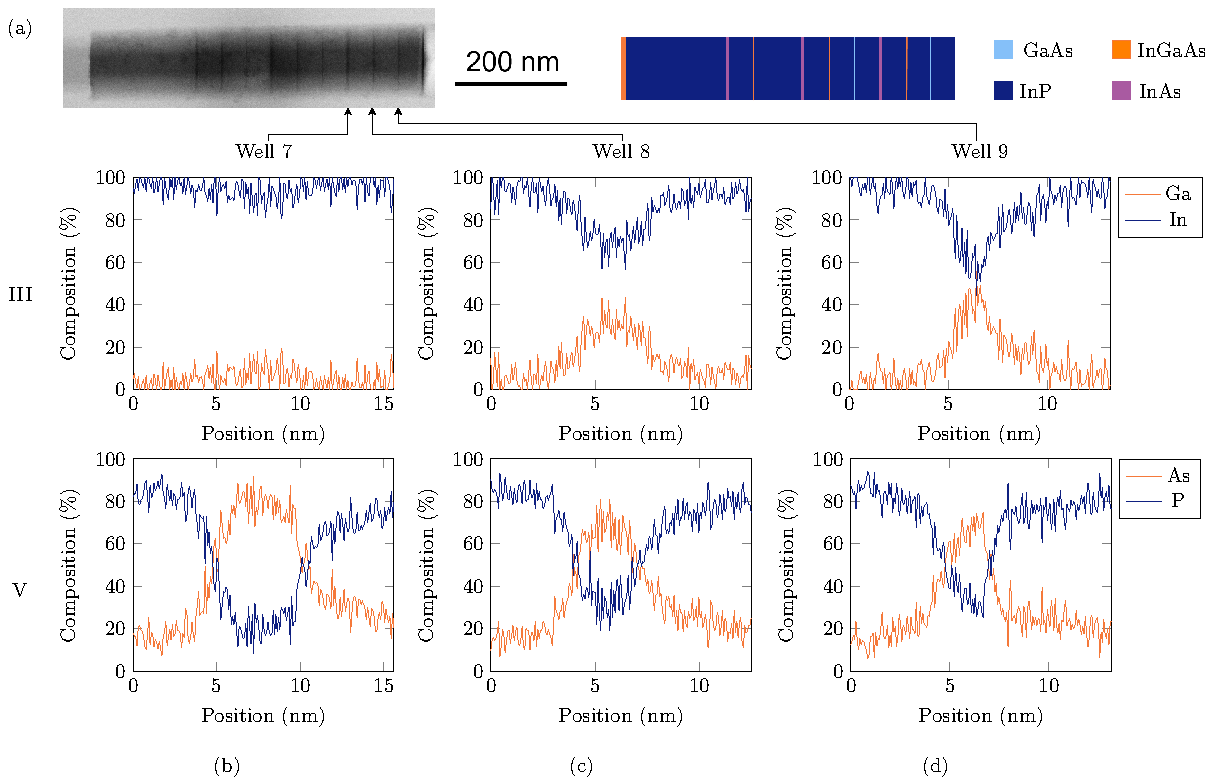
\includegraphics[width=\textwidth]{4_Properties/From_Article2/Figure5.pdf}
    \caption{Analysis of sample 2. (a) BF-STEM image of the III-V nanowire, \num{9} lines corresponding to the arsenide layers and corresponding schematic drawing with coloured layers indicating the design composition. Composition profiles for the 7th (b), 8th (c), and 9th (d) wells are calculated from EDS line scans carried out across the respective quantum well from left to right, in the direction parallel to the growth axis.}
    \label{fig:composition}
\end{figure}

A STEM and EDS analysis of sample 2 was conducted to assess the structuroptimisationnce of strained heterointerfaces (Figure~\ref{fig:composition}.a) on the growth of nanowires containing three \acs{inp}-\acs{inas}-\acs{inp}-\acs{ingaas}-\acs{inp}-\acs{gaas} heterolayer sequences. Figure~\ref{fig:composition}.b shows the results of the \acs{inas} layer, where onoptimisation V element precursor needs to be switched. The EDS profile indicates that this layer has formed as intended, with a phosphorus background level. 
\par
The \acs{ingaas} segment, with a target composition of \ce{In0_.53Ga0_.47As}, grew \acs{in}-rich, as seen from the EDS profiles in Figure~\ref{fig:composition}.c. A similar observation is made for the intended \acs{gaas} heterostructure: optimisation {fig:composition}.d shows this layer is heavily alloyed with a recorded \acs{in} molar fraction close to \num{0.5}. This indicates that the hold steps implemented in the growth recipe and designed to exhaust the group III element precursor (\acs{in}) were set too short. Further optimisation with prolongation of the purging step is thus suggested to improve composition control for these thin \qty{3}{nm}-wide heterostructures.
\par
The growth rates of the \acs{ingaas} and \acs{inp} layers were assessed with a process analogous to the one used for the growth rates of sample 1. The \acs{inp} growth rates is \qty[separate-uncertainty=true]{23.8 (0.3)}{\nano\metre\per\minute} between the first \acs{inas} and the first \acs{ingaas} wells and \qty[separate-uncertainty=true]{24.0 (0.4)}{\nano\metre\per\minute} between the third \acs{inas} and the third \acs{ingaas} wells. The \acs{ingaas} growth rates are \qty[separate-uncertainty=true]{39 (3)}{\nano\metre\per\minute} for the first \acs{ingaas} well and \qty[separate-uncertainty=true]{44 (2)}{\nano\metre\per\minute} for the third \acs{ingaas} well. All values are averaged from repeated measurements, and errors are given with 95\% certainty. Thus, the growth rates of samples 1 and 2 are comparable for these materials.


%\subsection{\texorpdfstring{Growth of wide \acl{qw} structures from multiple \acs{si} seeds}{Growth of wide quantum well structures from multiple Si seeds}}

%\begin{figure}
%    \centering
%    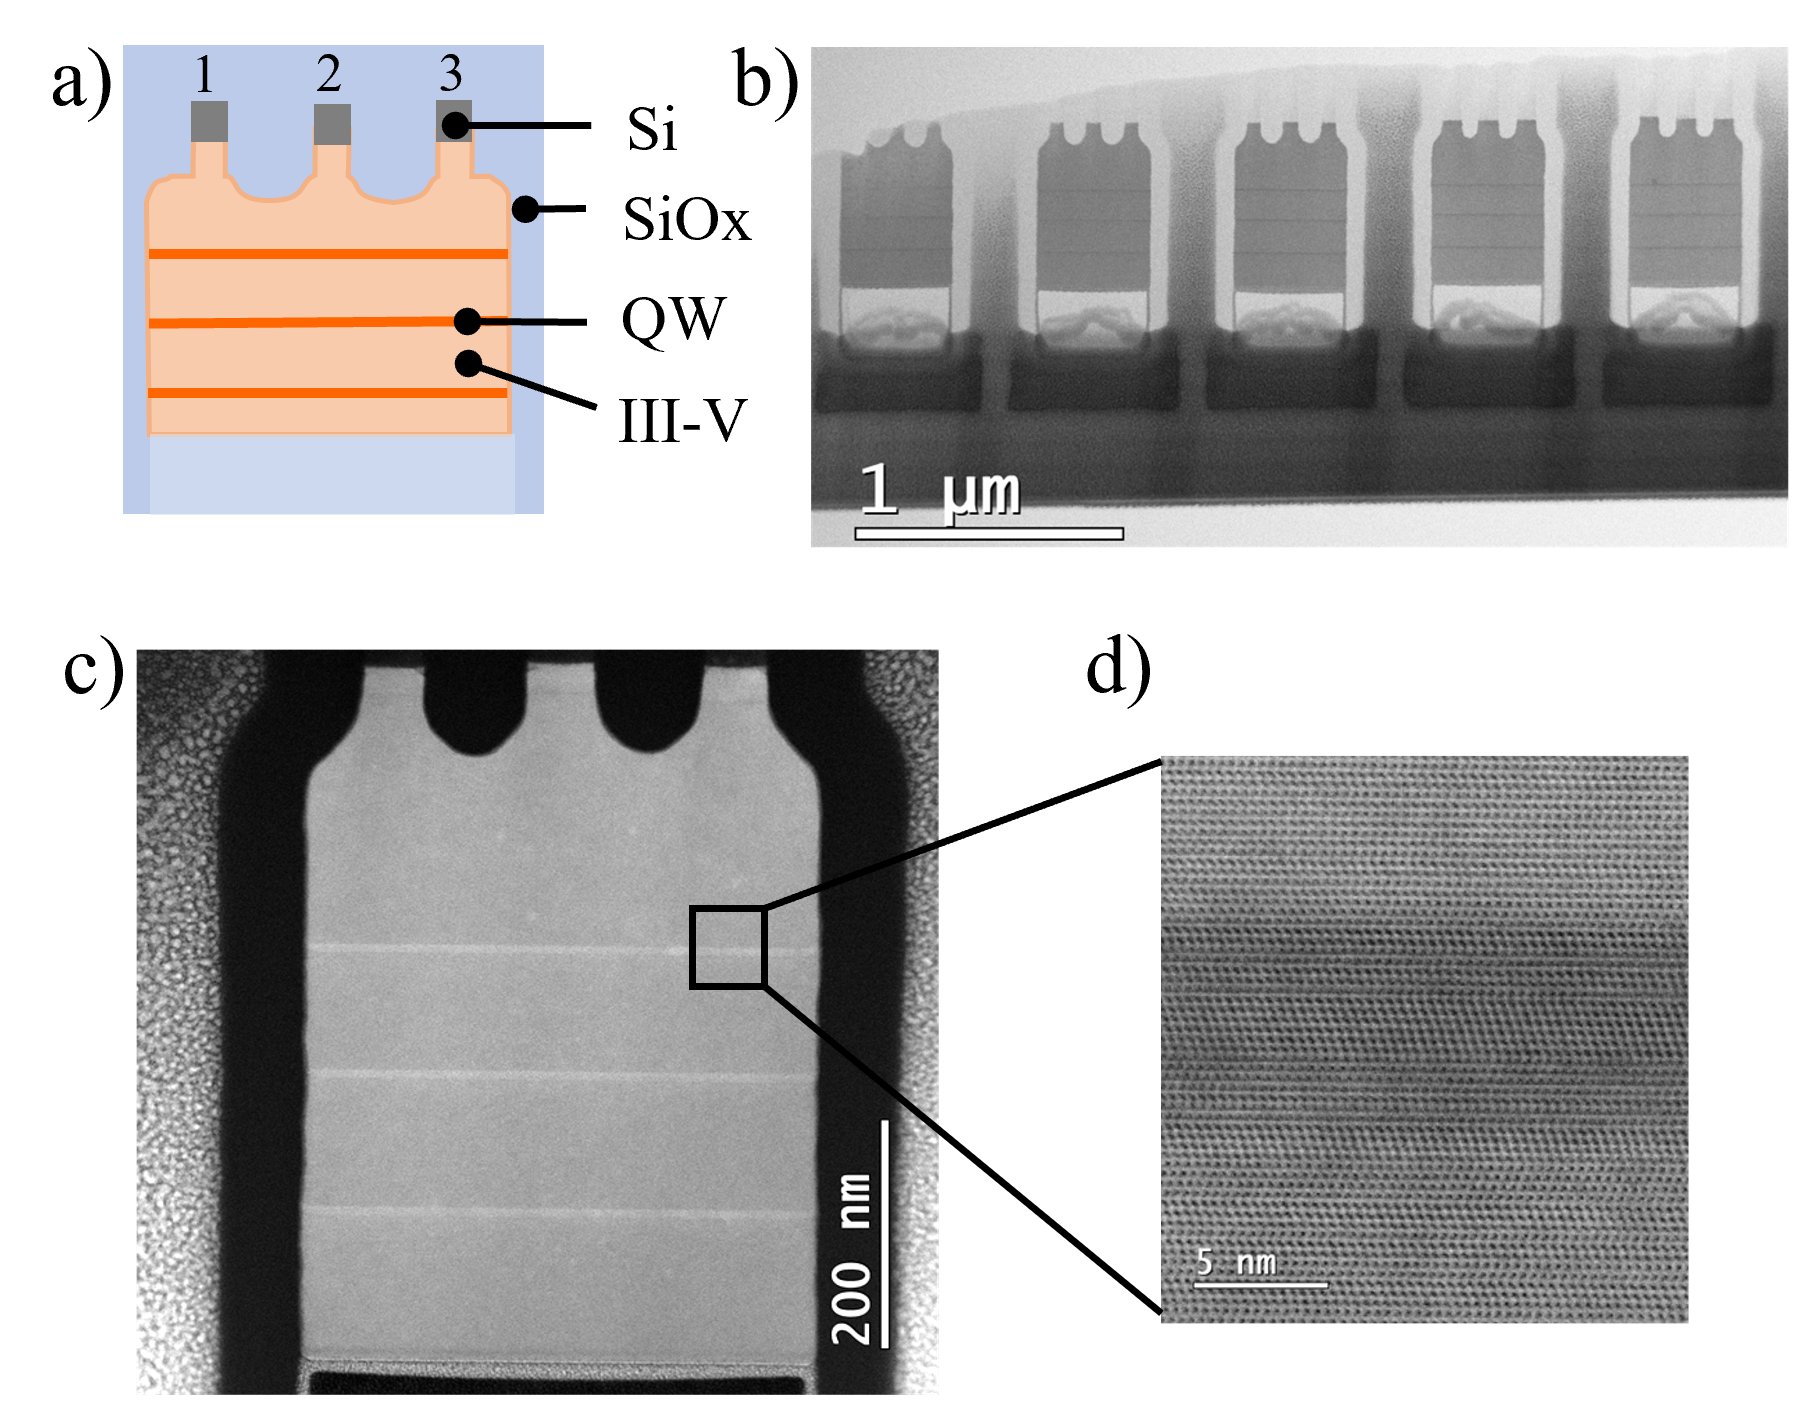
\includegraphics{4_Properties/From_Article2/Figure6.png}
%    \caption{STEM analysis of quantum wells created in wide structures from the multiple nucleation sites. (a) Top-view schematic of the structure. b) Plane-view image showing five adjacent structures (c) ADF-STEM image of one structure. (d) High-resolution BF-STEM image of a single quantum well.}
%    \label{fig:plane_view}
%\end{figure}

%To demonstrate the robustness of the developed epitaxy process as well as growth recipes, we fabricated test structures of larger width. Furthermore, the template contains not only one \acs{si} nucleation area, but three. Thus the III-V crystal is nucleated in three points simultaneously and develops into short nanowires. These nanowires are then forced to merge into one large platelet of well-defined geometry. The schematic of the structure is illustrated in Figure~\ref{fig:plane_view}.a.
%\par
%Figure~\ref{fig:plane_view}.b shows a BF-STEM plane-view image of five adjacent structures after STEM lamella preparation. The image shows a high consistency in the overall size of the grown structures and in the presence of the overall \num{15} quantum wells. A single structure is shown in Figure~\ref{fig:plane_view}.c using annular dark field (ADF-)STEM. The three light grey lines correspond to the \acs{ingaas} quantum wells. 
%The high-resolution BF-STEM image in Figure~\ref{fig:plane_view}.d shows one of these quantum wells appearing in darker grey, with additional contrast from alternating stacking sequences forming twin planes which are commonly observed for \hkl<111>\(_B\) growth\cite{Johansson2006}. The quantum well runs uniformly throughout the entire width of the structure, indicating that thevisualised this position took place on a single \hkl{111} plane. No other crystal defects were detected in STEM mode. To increase the sensitivity to detect structural defects, standard TEM analysis was performed as well (Figure~\ref{fig:TEM}).

%\begin{figure}
%    \centering
%    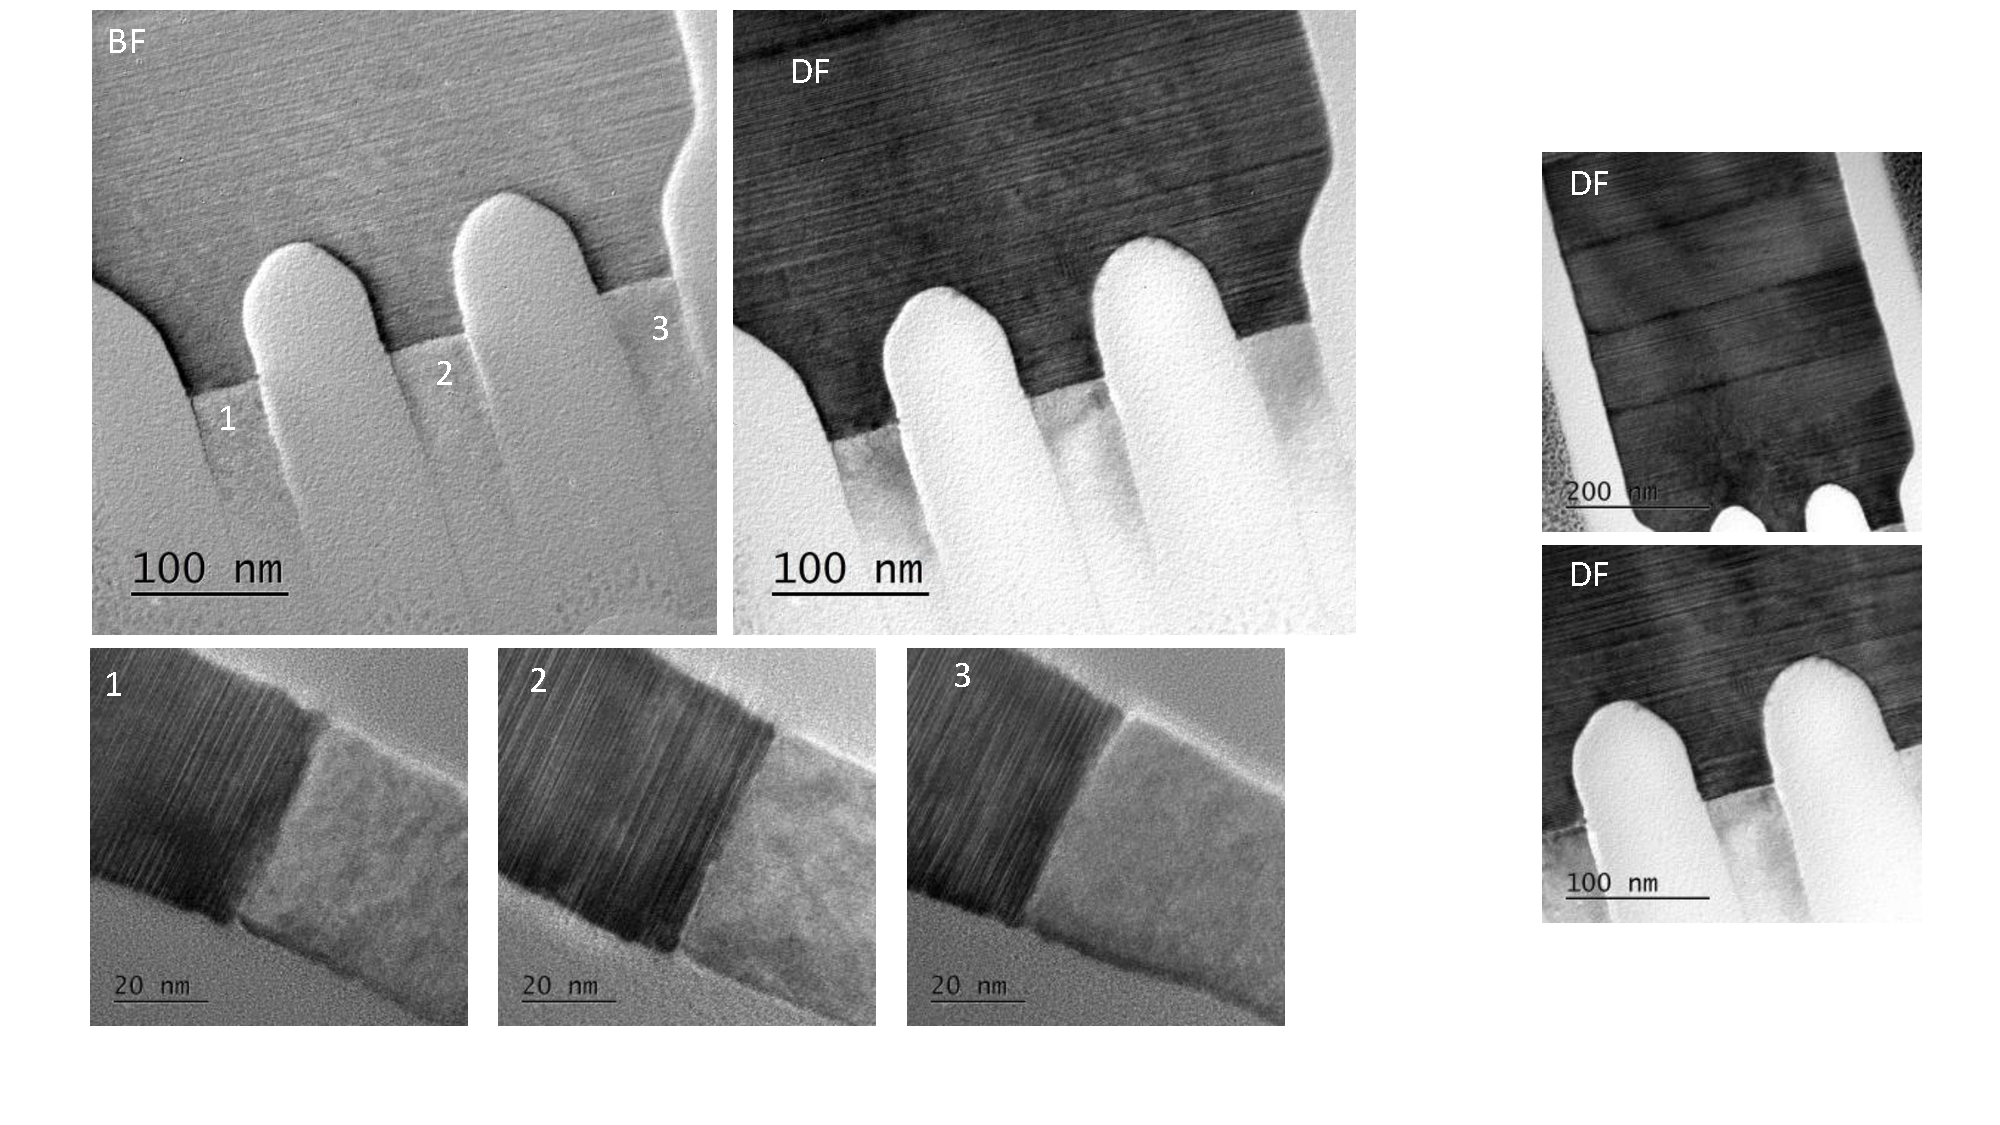
\includegraphics[width = \textwidth]{4_Properties/From_Article2/merging_analysis.pdf}
%    \caption{TEM analysis of the sampvisualisedFINITIVE FIGURE. PLEASE HEINZ, SEND RAW TEM IMAGES)}
%    \label{fig:TEM}
%\end{figure}

%No propagating dislocations or anti-boundary defects from merging the three initial crystals could be detected. However, this does not exclude the presence of lattice defects which could not be visualised under these imaging conditions. It is unlikely for the three crystal lattices to merge in a perfect registry without the formation of defects\cite{Jacobsson2015, Rossi2023}. However, here the resulting defects remain confined: growth of smooth quantum wells that extend straight across the entire width of the structure would otherwise be impossible.
%\par
%These observations can be explained by the specific sample geometry, growth directions, and material properties involved. The experiment is arranged in such a way that a \hkl{111}re-stabilisesont dominates, and no other growth planes are formed. This is achieved by setting a growth condition favouring slow growth along the main \hkl<111> direction and fast growth in the \hkl<110> directions. Under these conditions, efficient step flow occurs on the \hkl{111} facets. In such a configuration, the first wire to extend into the widening template section would spill over the spacre-stabilisesg it from the neighbouring wires and find itself supported on the other wire's \hkl{111} surface. Due to the efficient step flow on the \hkl{111} facets, mismatches of a few monolayers among the three wires are quickly resolved by the formation of one large growth surface that re-stabilises a single \hkl{111} growth front. A single crystal is established beyond these merging points, and growth can extend further into the template cavity.
%\par
%These structures share strong indications of local growth rate uniformity and simultaneous nucleation. The \num{5.7} width-to-height aspect ratio of Characterisationroduct{400 x 70}{nm} cross-section is higher than the \num{5} width-to-height aspect ratio (\qtyproduct{3000 x 500}{nm} cross-section) used by \citeauthor{Han2020} and shows a marked improvement in the control of shape and thickness of internal heterostructures. Further, our growth (carried out at \qty{580}{\degreeCelsius}) results are consistent with those obtained homoepitaxially at \qty{570}{\degreeCelsius} with a width-to-height cross-section of \num{20} by \citeauthor{Goswami2020}.

%\section{article1}
%\begin{figure}
%    \centering
%    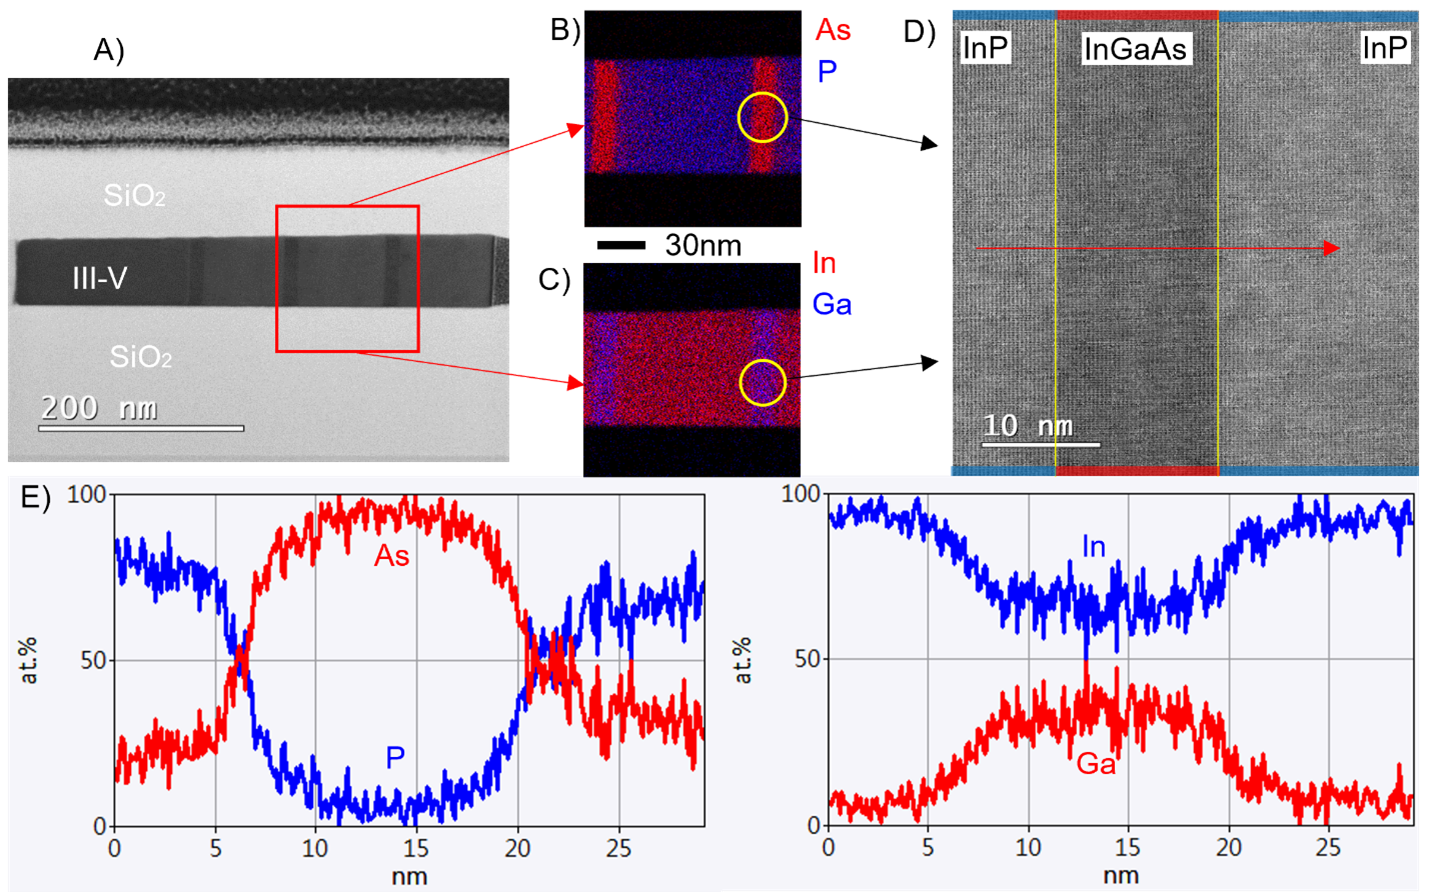
\includegraphics[width=\textwidth]{3_Growth/ICMOVPEXXFig5.png}
%    \caption{STEM image and EDS maps of a lamella cut from one of the nanowires grown on a <110> SOI. A) Overview of the BF-STEM image of the nanowire. The silicon seed is on the left, and silicon oxide is on the top and bottom. The entire heterostructure stack is visible due to channelling contrast: InGaAs appear darker than InP. B) Color-coded EDS map of the region highlighted by the red square in (A): in red In concentration and blue Ga concentration. C) Color-coded EDS map of the region highlighted by the red square in (A): red As concentration and blue P concentration. D) High-resolution BF-STEM detail of the 10-nm-thick InGaAs well. E) EDS line-scan spectra recorded across the InGaAs and highlighted in (D) by the red arrow showing scan direction.}
%    \label{fig:ICMOVPEXXFig5}
%\end{figure}

%In the previous examples, a <001> device layer SOI was used as a growth substrate, where a multi-faceted growth front can develop, leading to poor geometric control, composition variations for ternaries, and in any case, a heterointerface which is not perpendicular to the growth direction, which is an undesirable situation for device fabrication. This can be circumvented using a Si wafer orientation with vertical {111} crystal planes as available on an <110> SOI wafer—

%hfigure 5. A shows a BF-STEM image of a nanowire with vertical and well-defined hetero-interfaces. 

%A similar level of As background impurities is present after each InGaAs segment, as shown in Figure 5. B, while Figure 5. C shows how Ga is well confined to the respective layer. 

%The high-resolution BF-STEM image in Figure 5.D shows the heterointerface between the 85-nm-thick InP on the image's left- and right-hand side and the 14-nm-thick InGaAs quantum well structure that appears as a dark layer in the middle of the image. The extracted <111>B growth rates are 25.5 nm/min for InP and 42.9 nm/min for InGaAs, respectively. This marks an increase in growth rate attributed to the different template shapes, as template height was reduced from 220 nm to 70 nm—

%figure 5. E shows the composition profiles for the III- and group elements across the quantum well region. The presence of As impurities immediately after the quantum well layer is again noticeable on the right side of the V element map, as the As and P concentration profiles are asymmetric. This asymmetry is evident when compared with the symmetric composition profiles for the III-group elements, which maintain the interface quality observed in the sample shown in Figure 4. The III composition profile Figure 5. E highlights how the InxGa1-xAs composition is more prosperous in Indium, having an x = 0.60. As the flows into the reactor were not altered from the sample shown in Figure 4, this composition change can also be attributed to the different template geometry.